\section{Event Selection}
\label{sec:selection}

Events with signatures consistent with $\ttbar$ production and large $\met$ are selected. An excess in the tails of the $\met$ distribution over SM expectations could indiciate the production of DM particles. Two final states have been studied,
\begin{itemize}
\item \textbf{Hadronic:} jets$+\met$ final state where the $\W$ daughters from the tops decay hadronically,
\item \textbf{Semileptonic:} $\Lep+$jets$+\met$ final state where one of the $\W$ daughters from the tops decay leptonically into a muon or electron and neutrino.
\end{itemize}

%Recent developments in jet substructure have established effective techniques for identifying highly boosted $\Top$ quarks that decay hadronically such that all decay products fall within a single jet. This allows definitions of signal region categories with higher purity in the kinematic regime of boosted tops. Therefore, two general selection strategies are presented:
Two exclusive categories are presented:
\begin{itemize}

\item \textbf{Inclusive:} a single signal category that does not target any kinematic region in particular.
\item \textbf{Top-tagged:} the signal region is comprised of resolved top tags.%divided into several categories based on the number of boosted top tags.
\end{itemize}

\subsection{Inclusive Selection: Hadronic channel}
\label{subsec:sel_incl_hadronic}
%\textcolor{red}{To be updated from Phys14 to Spring15 studies before full stats}
Events for the hadronic channel are obtained with two triggers. For events from runs before 254227, the trigger used is HLT\_PFMET170\_NoiseCleaned\_PFMHTNoMu120\_IDTight, while for subsequent runs, the trigger is HLT\_PFMETNoMu120\_JetIdCleaned\_PFMHTNoMu120\_IDTight. The efficiency of these triggers with respect to offline $\met$ in the single electron and single muon channels is shown in Fig.~\ref{fig:meteff_0}. Discrepancies in the turn-on curves between the two channels are under investigation. Overall efficiencies at the plateau in both channels are in agreement between data and MC (comparing the fit parameter $\epsilon_{0}$ and the fit).This dictates the use of a unity scale factor for data-to-MC $\met$ corrections.

\begin{figure}[htbp]
\centering
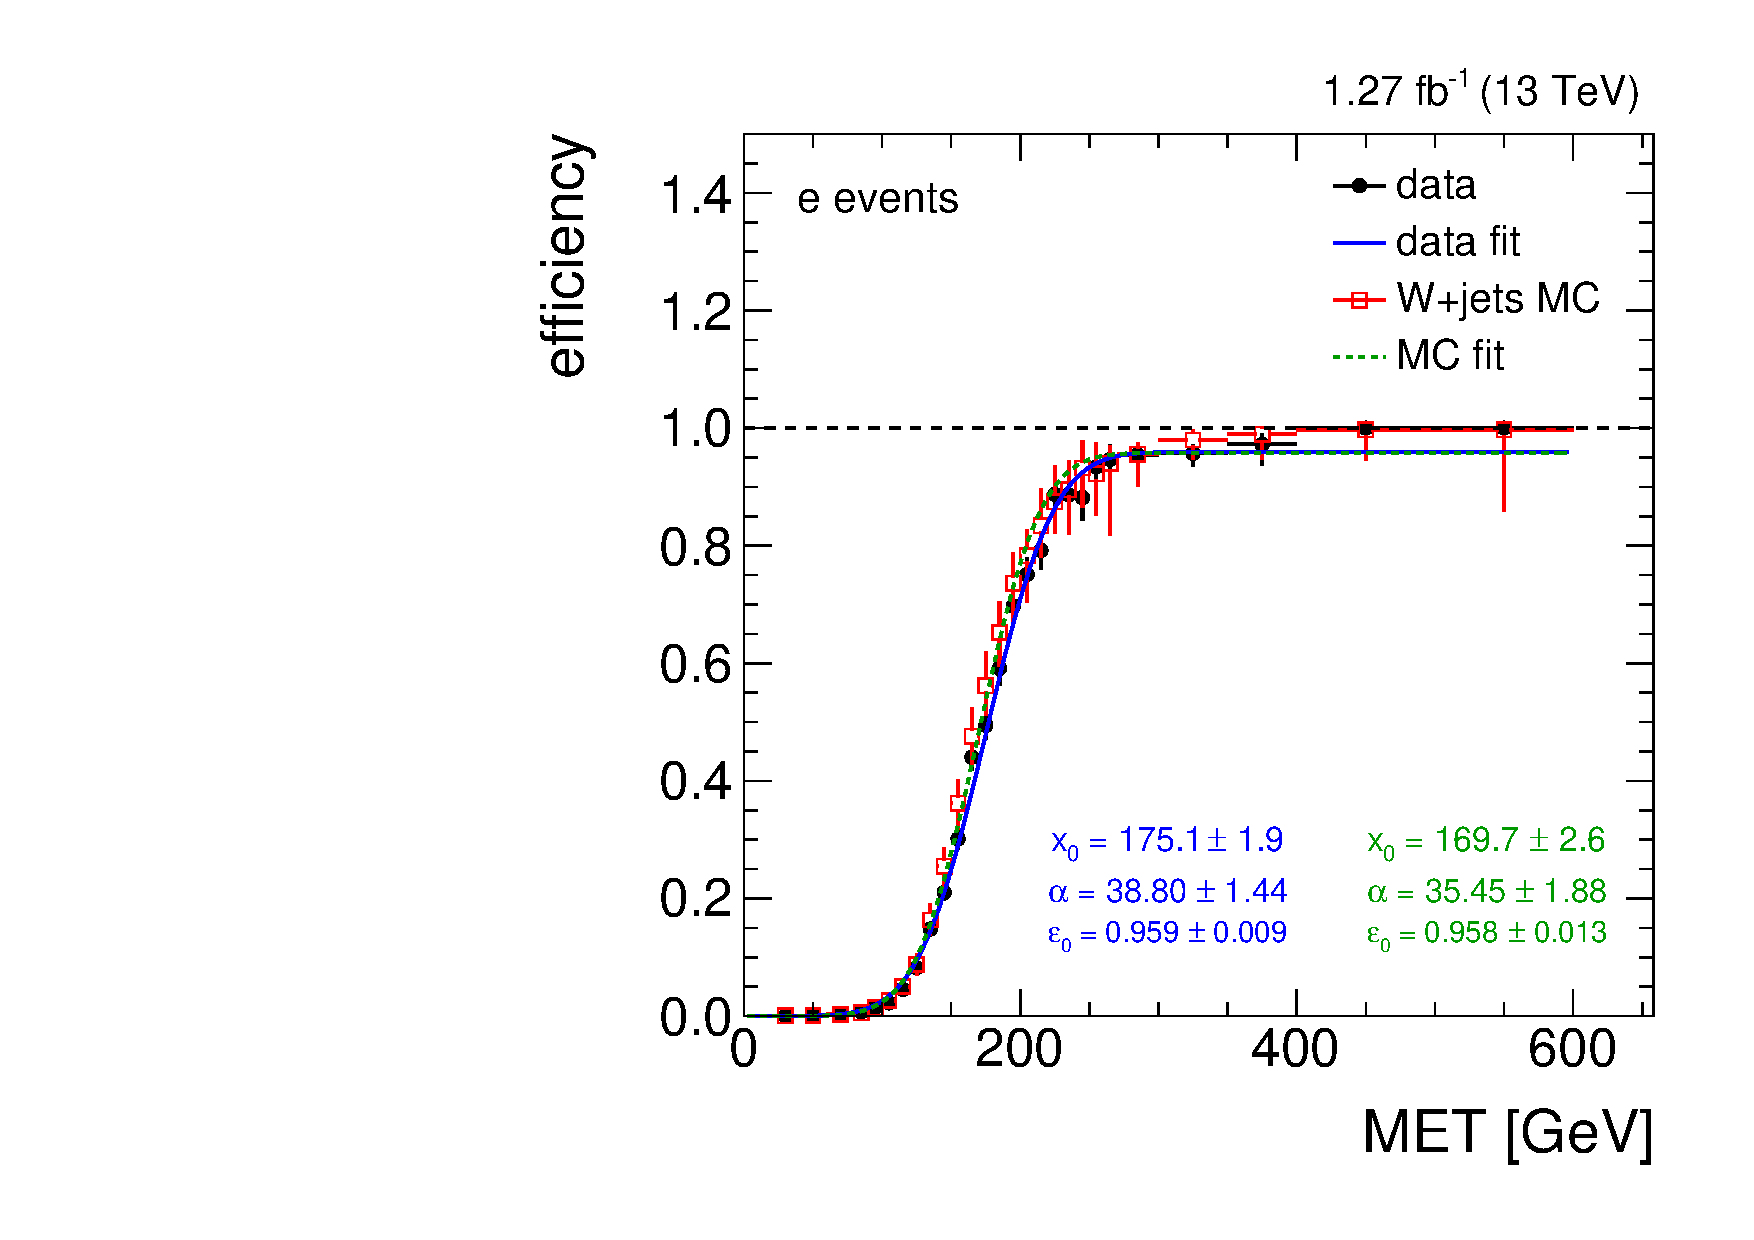
\includegraphics[width=0.48\textwidth]{figures/meteff_e_1.pdf}
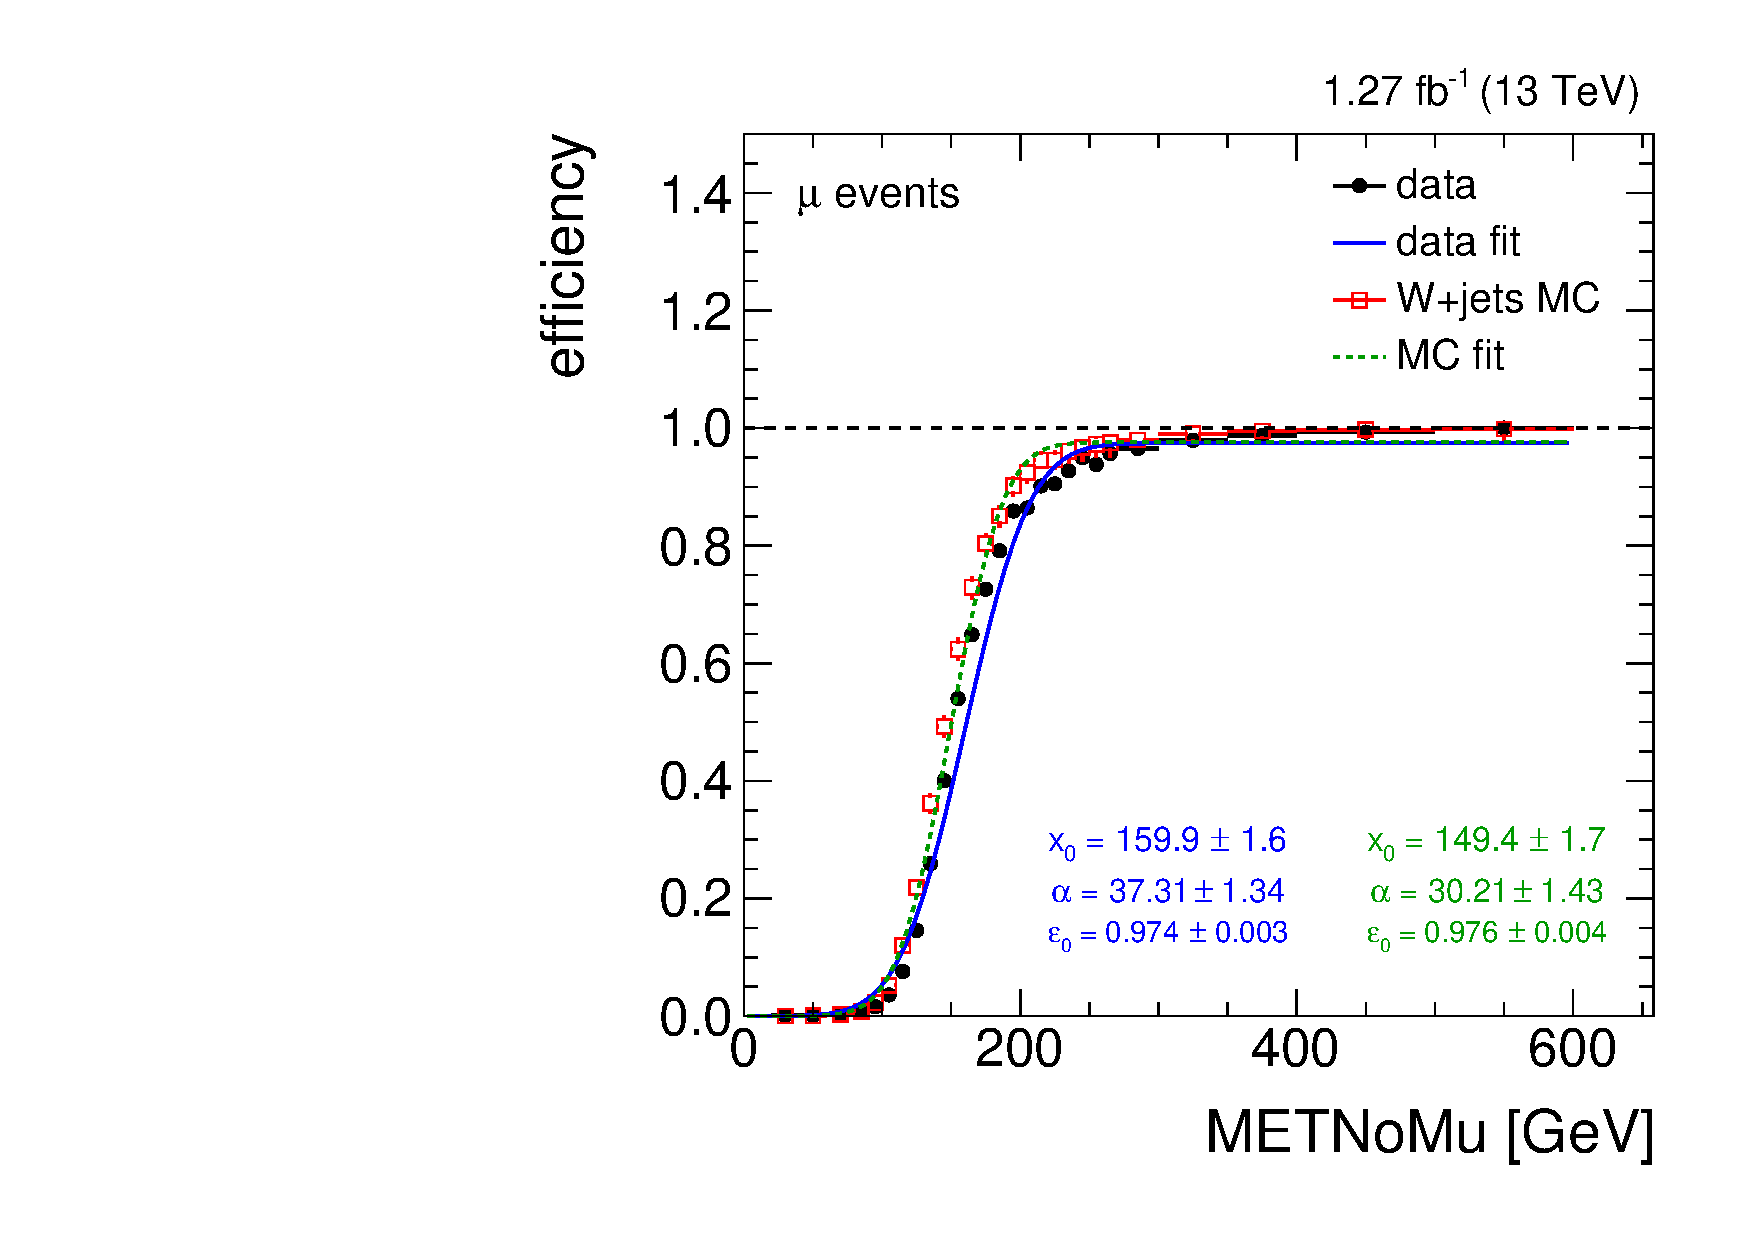
\includegraphics[width=0.48\textwidth]{figures/meteff_m_1.pdf}
\caption{Efficiency turn-on curves of HLT\_PFMET170\_NoiseCleaned\_PFMHTNoMu120\_IDTight and HLT\_PFMETNoMu120\_JetIdCleaned\_PFMHTNoMu120\_IDTight for electron events (left) and muon events (right). Events are required to have at least four jets.}
\label{fig:meteff_0}
\end{figure}

\begin{figure}[htbp]
  \centering
  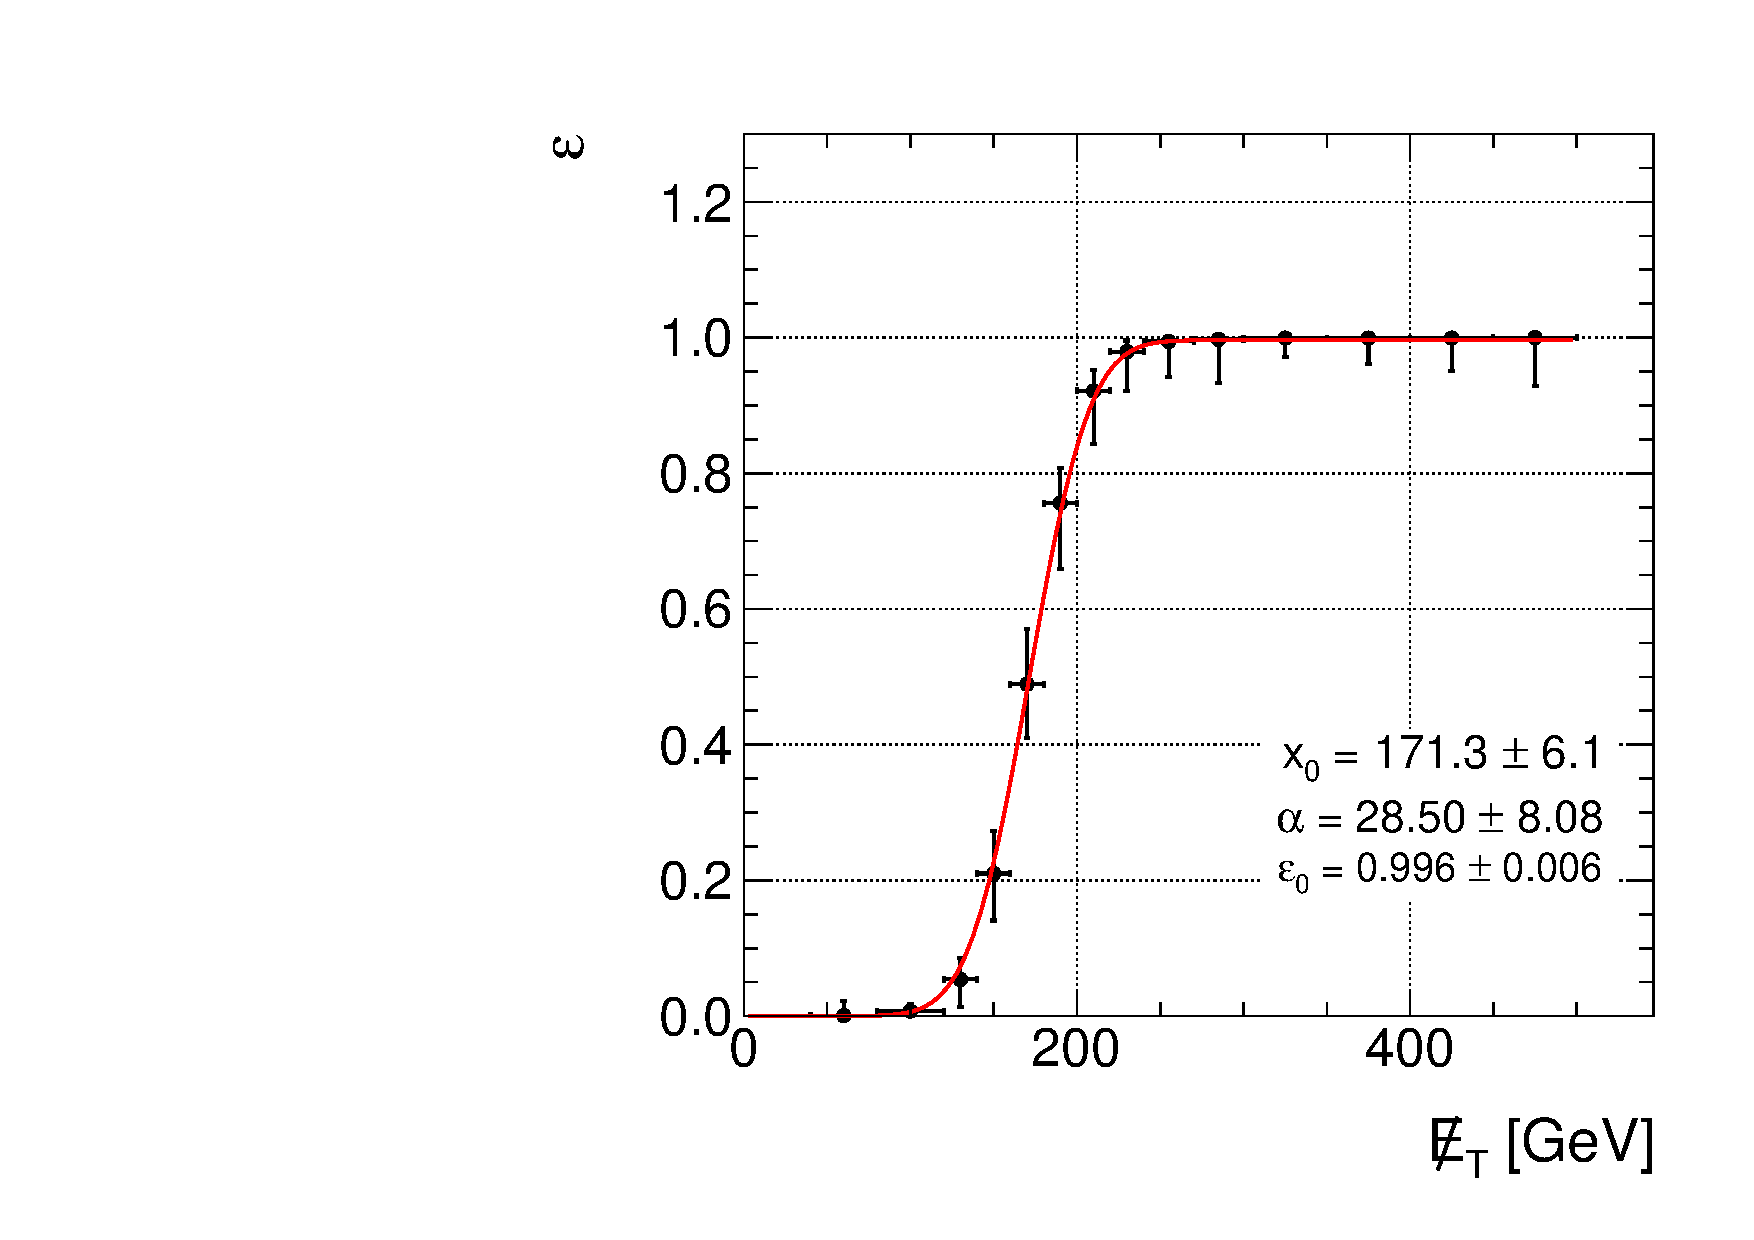
\includegraphics[width=0.48\textwidth]{figures/ttdm1-meteff.pdf}
  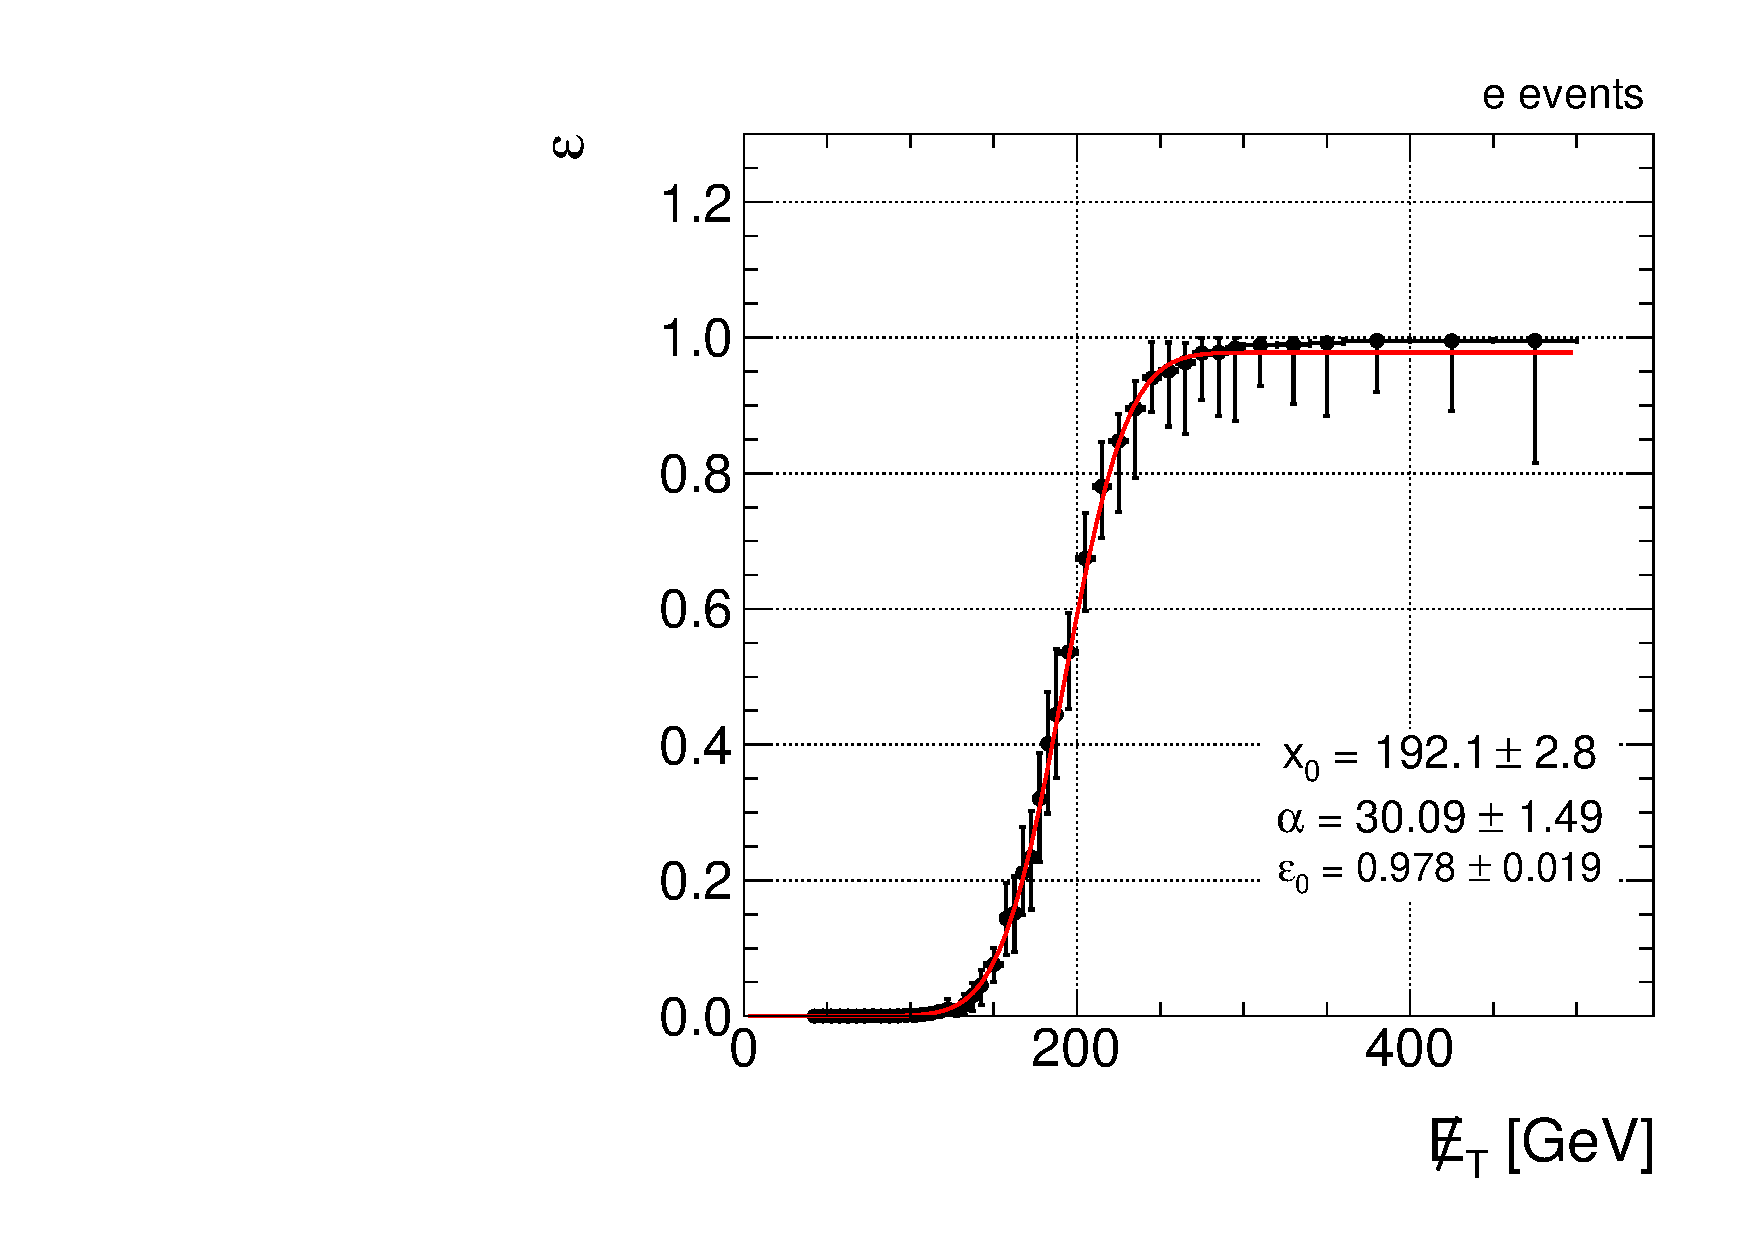
\includegraphics[width=0.48\textwidth]{figures/wjets-e-meteff.pdf}
  \caption{Efficiency turn-on curves of HLT\_PFMET170\_NoiseCleaned for $\ttbar+$DM EFT signal with $M_{\chi}=1$ (left), and for electron events in $\Wjets$ passing a single electron trigger (right). Events are required to have at least four jets.}
  \label{fig:meteff_1}
\end{figure}

The offline event selection requires,
\begin{itemize}
\item $\met > 250\:\GeV$, to be on the plateau of the efficiency turn-on curve,
\item at least $4$ AK4CHS jets with $\pt>30\:\GeV$ and $|\eta|<4$,
  \begin{itemize}
  \item at least $2$ of which have $|\eta|<2.4$ and $\Bot$-tagged,
  \end{itemize}
\item no muons passing ``Loose'' selection with $\pt>10\:\GeV$ and $|\eta|<2.4$,
\item no electrons passing ``Veto'' selection with $\pt>10\:\GeV$ and $|\eta|<2.5$,
\item $\min_{i=1,\ldots,6}\Delta\phi\left(j_i,\met\right)>1$, the minimum $\Delta\phi$ between jet and $\met$ considering up to the sixth leading jet.
\end{itemize}

The $\min_{i=1,\ldots,6}\Delta\phi\left(j_i,\met\right)$ distribution after all other selection cuts is shown in Fig.~\ref{fig:dphijetmet6}. The cut on this variable reduces the QCD multi-jets background to negligible levels. It also reduces the $\ttbar$ background, which is predominantly semileptonic.%, because events with high $\met$ have a boosted $\Top$ quark and therefore the neutrino and $\Bot$ jet will be close to each other. 
It was studied that considering $\Delta\phi$ for up to the sixth leading jet performs better than considering fewer number of jets and better than considering all jets. These studies are presented in Appendix~\ref{app:dphijetmet}.

\begin{figure}[htbp]
  \centering
  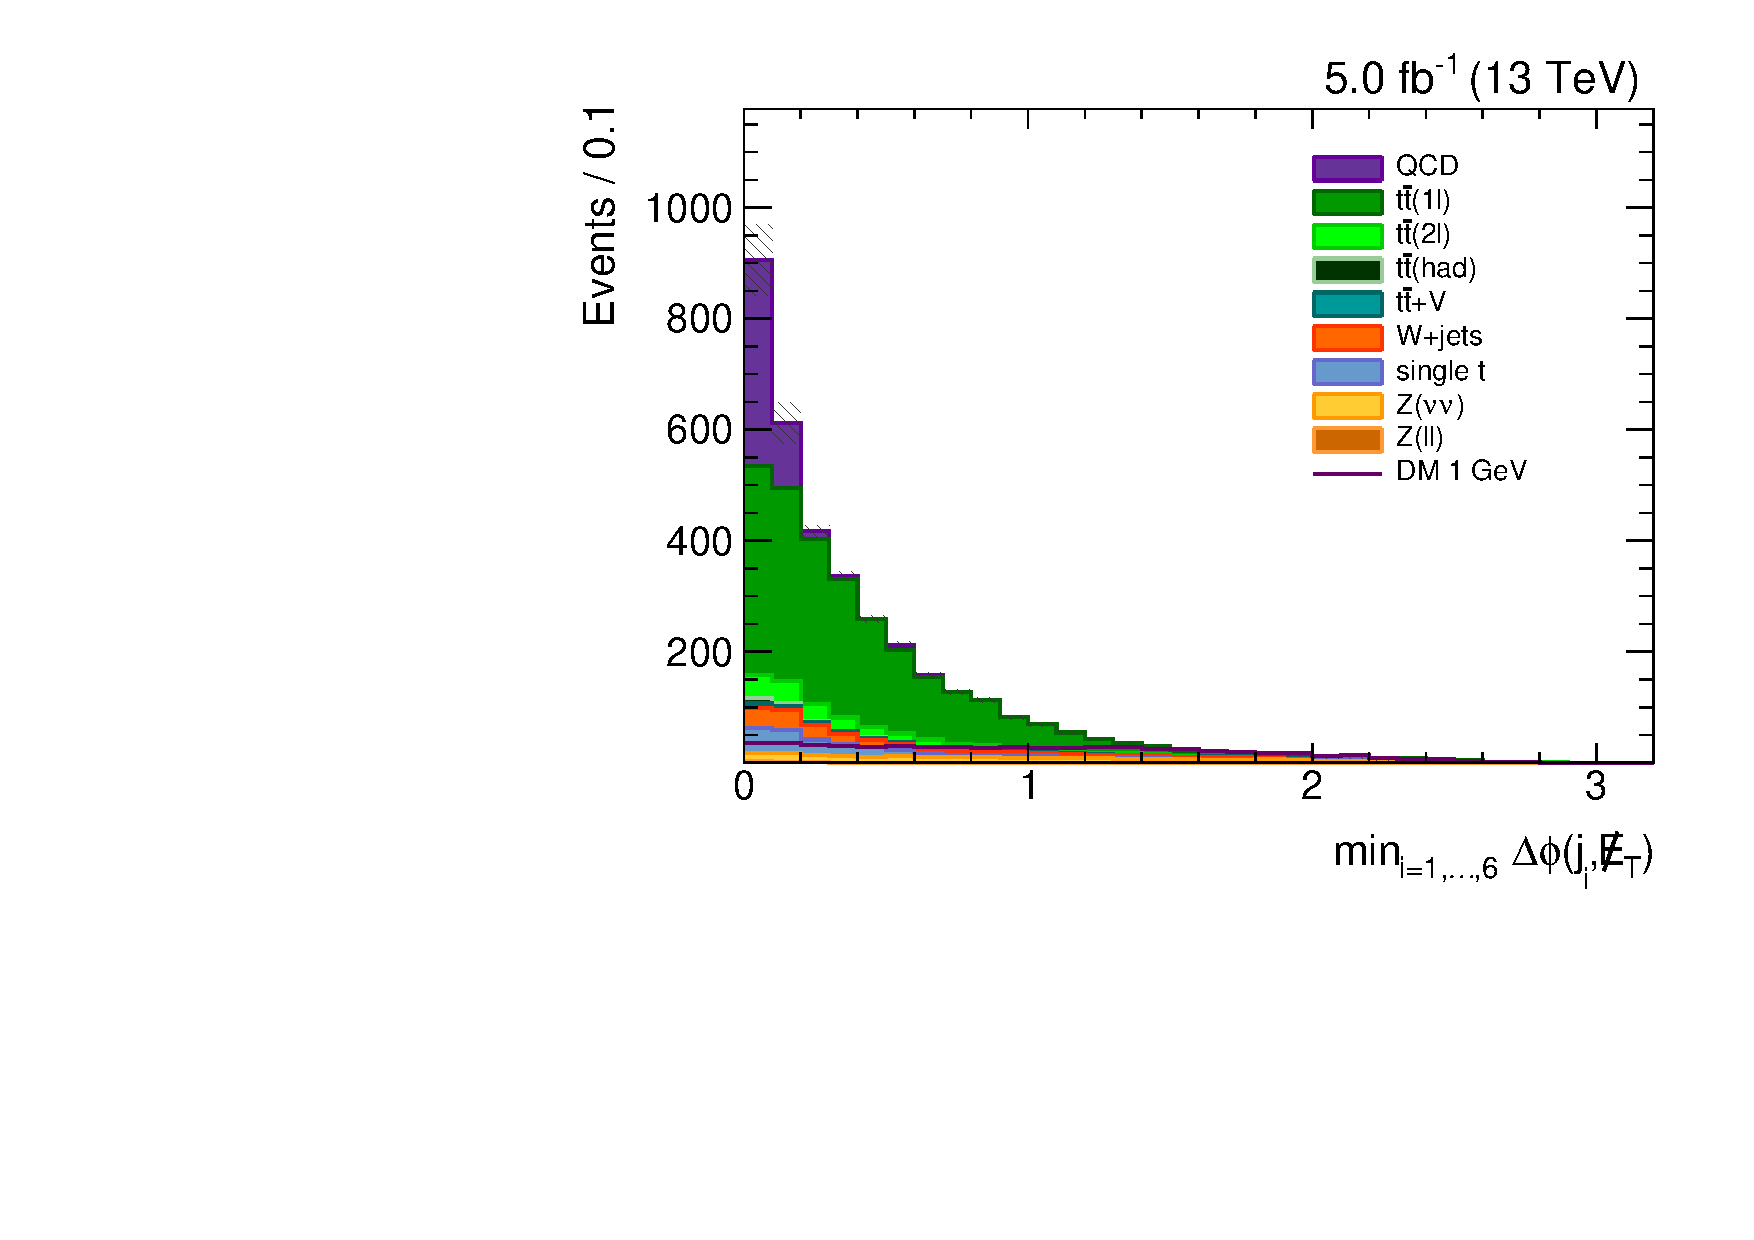
\includegraphics[width=0.48\textwidth]{figures/hadronic-incl-dphijetmet6.pdf}
  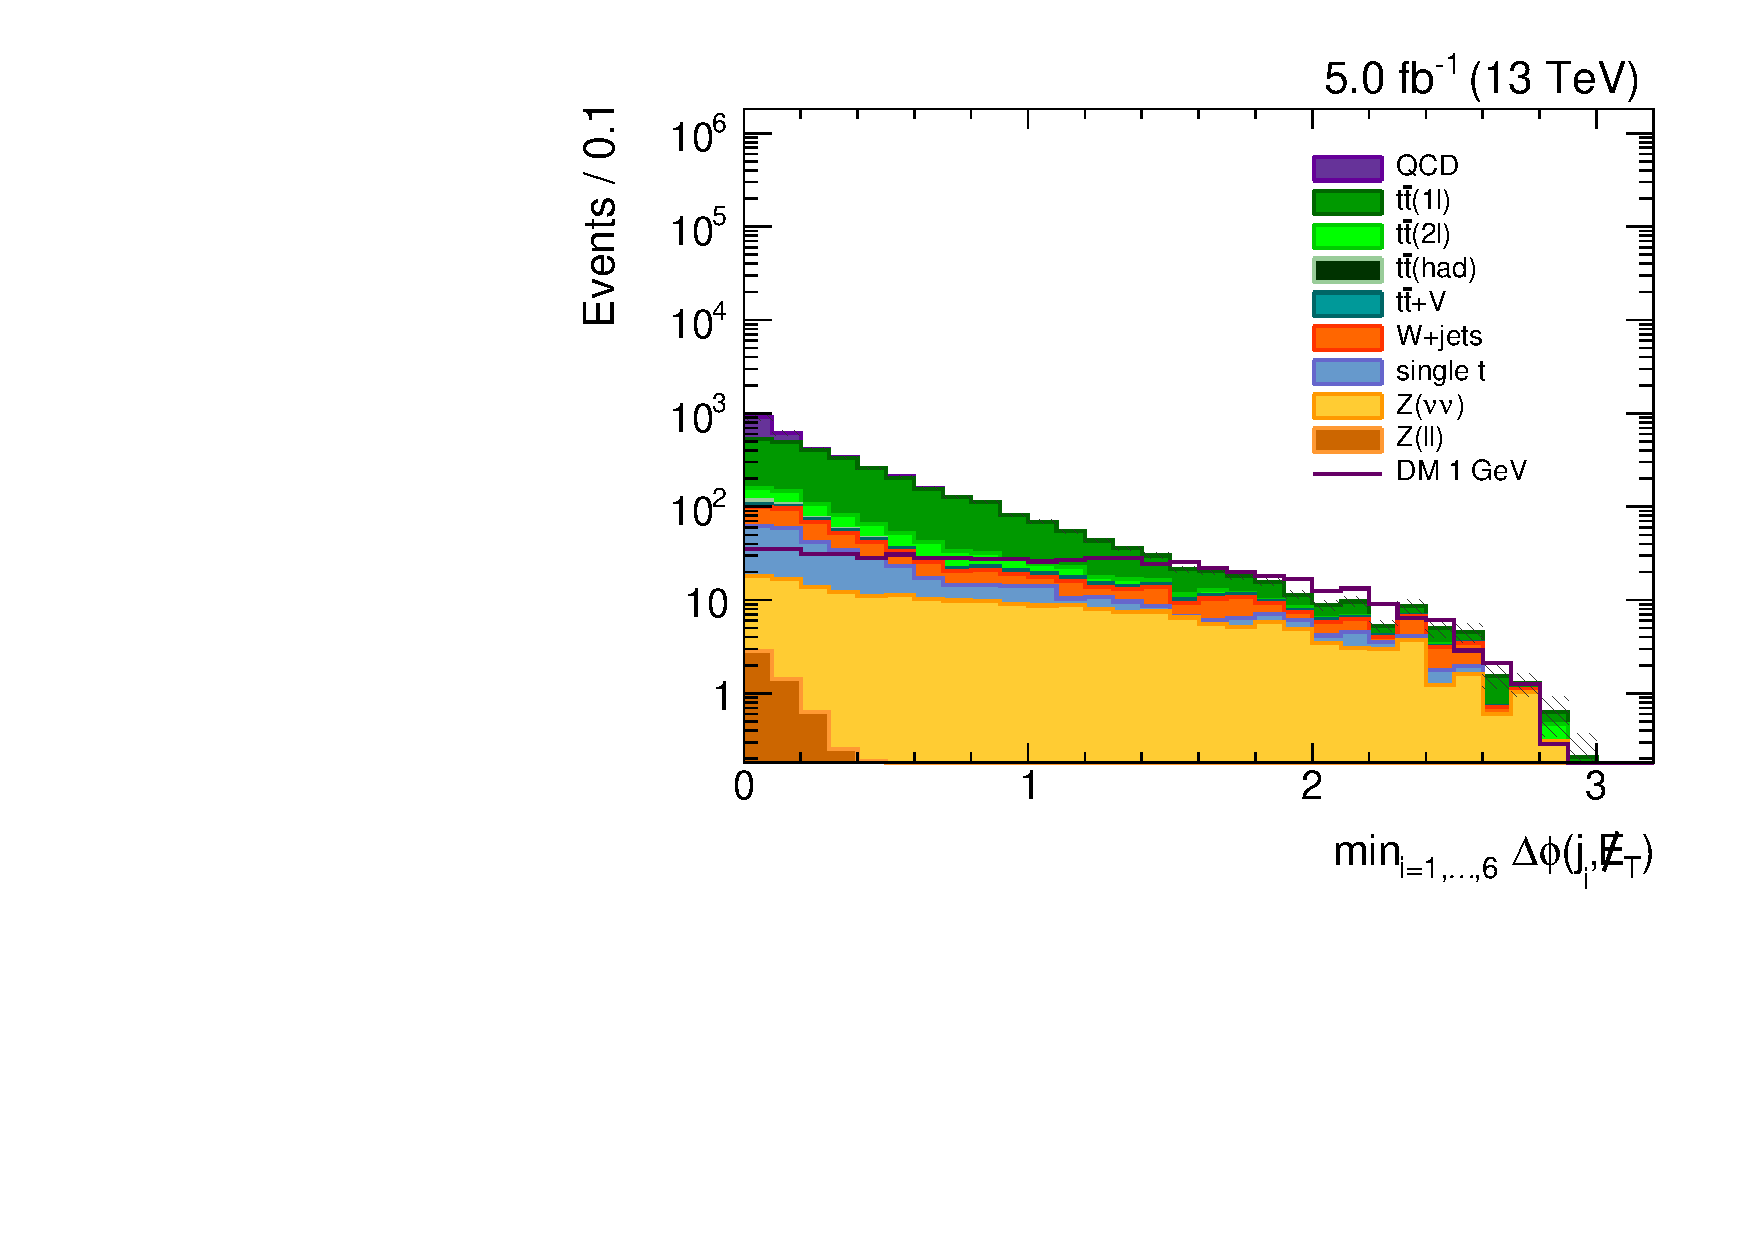
\includegraphics[width=0.48\textwidth]{figures/hadronic-incl-dphijetmet6log.pdf}
  \caption{The $\min_{i=1,\ldots,6}\Delta\phi\left(j_i,\met\right)$ distribution in linear scale (left) and log scale (right).}
  \label{fig:dphijetmet6}
\end{figure}

The $\met$ distributions before and after cutting on $\min_{i=1,\ldots,6}\Delta\phi\left(j_i,\met\right)$ are shown in Fig.~\ref{fig:incl_hadronic_met}. The expected yields for $5\:\ifb$ after selection are shown in Table~\ref{tab:incl_hadronic_yields}.

\begin{figure}[htbp]
  \centering
  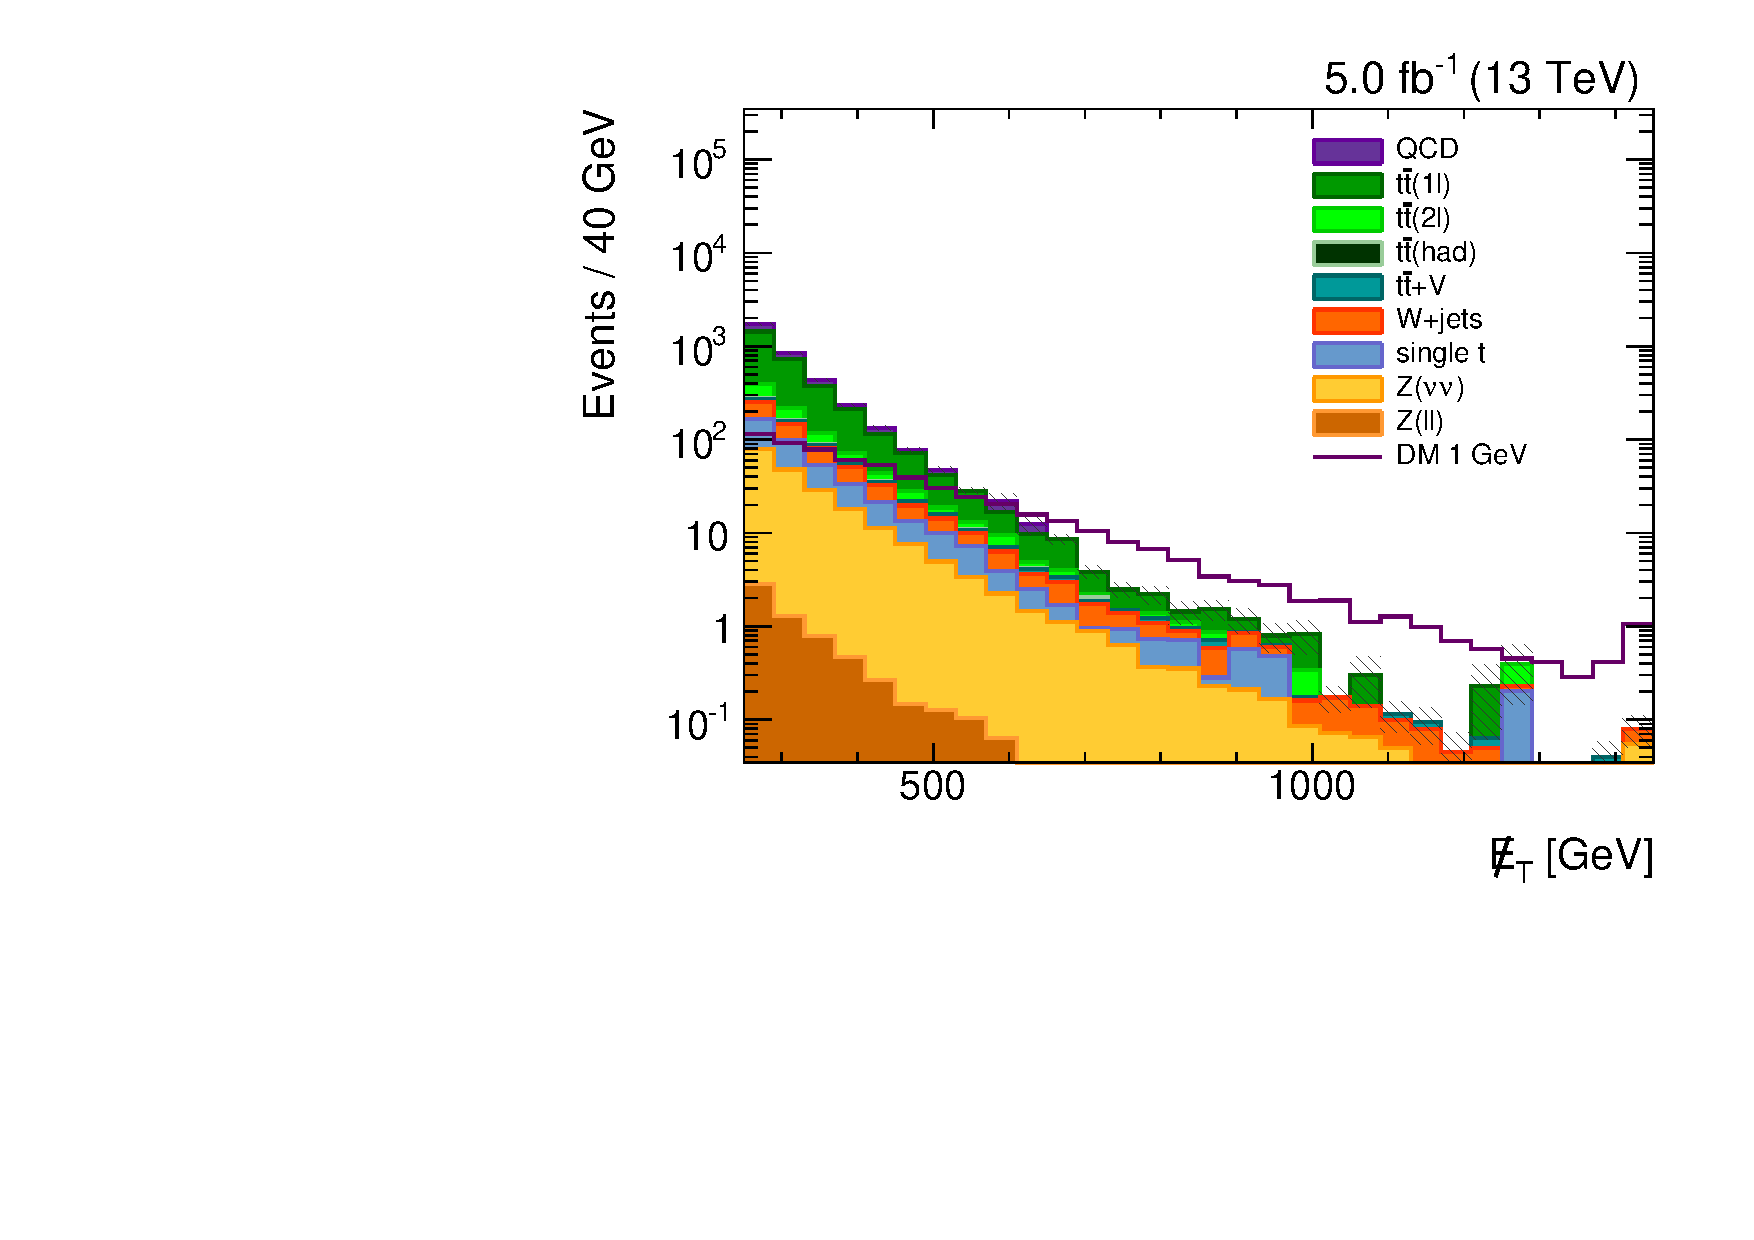
\includegraphics[width=0.48\textwidth]{figures/hadronic-incl-metlog_nodphi.pdf}
  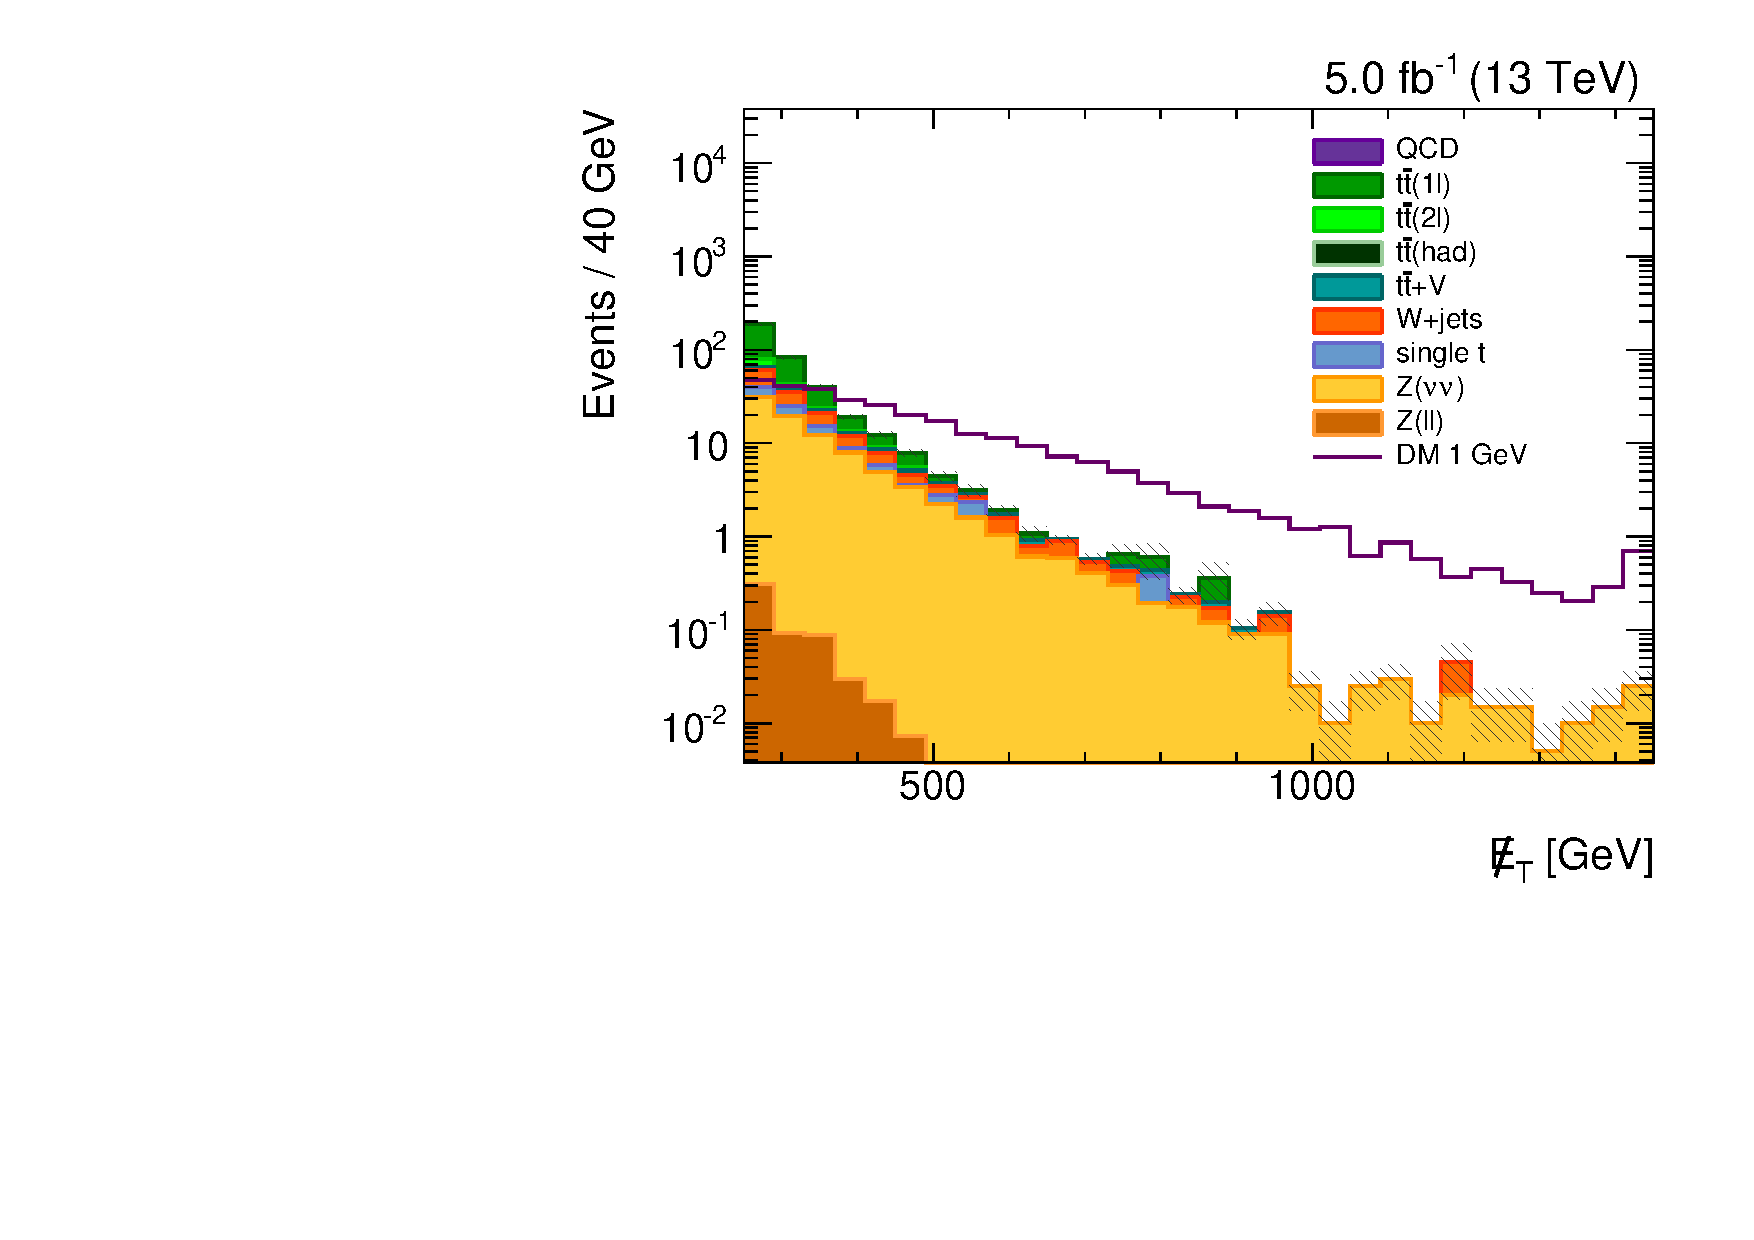
\includegraphics[width=0.48\textwidth]{figures/hadronic-incl-metlog.pdf}
  \caption{The $\met$ distribution before (left) and after (right) the cut on $\min_{i=1,\ldots,6}\Delta\phi\left(j_i,\met\right)$. Note that the right-most bin includes overflow.}
  \label{fig:incl_hadronic_met}
\end{figure}

\begin{table}[!ht]
\centering
\begin{tabular}{|c|r|}
\hline
  Process               & \multicolumn{1}{|c|}{Yields} \\
\hline
  \Z\To\Lep\Lep         & $  0.54 \pm 0.12$ \\
  \Z\To\Nu\Nu           & $ 86.09 \pm 1.82$ \\
  Single \Top           & $ 21.36 \pm 1.89$ \\
  \Wjets                & $ 45.42 \pm 3.11$ \\
  QCD                   & $  0.00 \pm 0.00$ \\
  $\ttbar+V$            & $ 11.19 \pm 0.40$ \\
  $\ttbar(\mbox{had})$  & $  0.00 \pm 0.00$ \\
  $\ttbar(1\Lep)$       & $179.61 \pm 5.42$ \\
  $\ttbar(2\Lep)$       & $ 21.74 \pm 1.88$ \\
\hline
  SM expected           & $365.94 \pm 7.04$ \\
\hline
  $M_\chi=1\:\GeV$      & $289.61 \pm 3.45$ \\
\hline
\end{tabular}
\caption{Expected yields for $5\:\ifb$ after the inclusive selection for the hadronic channel.}
\label{tab:incl_hadronic_yields}
\end{table}

\subsection{Inclusive Selection: Semileptonic channel}
\label{subsec:sel_incl_semilept}

Events for the semileptonic channel are obtained with HLT\_Ele27\_eta2p1\_WP75\_Gsf in MC and HLT\_Ele27\_eta2p1\_WPLoose\_Gsf in data, a single electron trigger, and HLT\_IsoMu27, a single muon trigger. Kinematic thresholds on the trigger objects constrain the offline requirements on the electron or muon to $\pt>30\:\GeV$ and $|\eta|<2.1$ in order to avoid the sharp efficiency turn-on. Trigger efficiencies measured with the tag-and-probe method are shown in Fig.~\ref{fig:seleff} and Fig.~\ref{fig:smueff} for the single electron HLT\_Ele27\_eta2p1\_WP75\_Gsf trigger measured in MC and HLT\_Ele27\_eta2p1\_WPLoose\_Gsf in data and HLT\_IsoMu27 in data and MC, respectively.

The data-to-MC trigger efficiency scale factors for the single electron HLT\_Ele27\_eta2p1\_WP75\_Gsf trigger and the single muon HLT\_IsoMu27 trigger have been computed in $\pt$-$|\eta|$ bins using standard tag-and-probe procedures and are shown in Table~\ref{tab:sf_ele} and Table~\ref{tab:sf_mu} respectively. 

\begin{table}[!ht]
\centering
\begin{tabular}{|c|c|c|c|c|}
\hline
&                                &                                &                                &                                                                 \\   
& $0.0 < |\eta| < 0.4$ & $0.4 < |\eta| < 1.4$ & $1.4 < |\eta| < 1.6$ & $1.6 < |\eta| < 2.1$    \\
&                                &                                &                                &                                                                \\   
\hline
$30 < \pt <  32$ &  $0.936 \pm  0.006$  &  $0.947 \pm  0.006$  &  $0.794 \pm  0.026$  &  $0.893 \pm  0.008$ \\
\hline
$32 < \pt <  35$ &  $0.958 \pm  0.003$  &  $0.980 \pm  0.003$  &  $0.914 \pm  0.013$  &  $0.954 \pm  0.005$ \\
\hline
$35 <\pt  <  40$ &  $0.970 \pm  0.002$  &  $0.998 \pm  0.001$  &  $0.999 \pm  0.006$  &  $0.958 \pm  0.003$ \\
\hline
$40 < \pt <  50$ &  $0.980 \pm  0.001$  &  $1.005 \pm  0.001$  &  $0.998 \pm  0.004$  &  $0.958 \pm  0.002$ \\
\hline
$50 < \pt < 200$ & $0.998 \pm  0.001$  &  $1.012 \pm  0.001$  &  $1.004 \pm  0.005$  &  $0.944 \pm  0.003$ \\
\hline
      $\pt > 200$   & $1.011 \pm  0.031$  &  $1.012 \pm  0.019$  &  $0.947 \pm  0.115$  &  $0.950 \pm  0.077 $\\	
\hline	
	
\end{tabular}
\caption{Data-to-MC efficiency scale factors for single electron trigger by $\pt$-$|\eta|$ bins}
\label{tab:sf_ele}
\end{table}


\begin{table}[!ht]
\centering
\begin{tabular}{|c|c|c|c|c|c|c|}
\hline
  &                                &                                &                                &                                 &                                &                             \\   
  & $0.0 < |\eta| < 0.4$ & $0.4 < |\eta| < 0.8$ & $0.8 < |\eta| < 1.2$ & $1.2 < |\eta| < 1.6$ & $1.6 < |\eta| < 2.1$ & $2.1 < |\eta| < 2.4$ \\
  &                                &                                &                                &                                 &                                &                             \\   

\hline
	$30 < \pt <   32$ &  $0.963 \pm  0.004$  & $ 1.004 \pm  0.003 $ &  $0.982 \pm  0.005 $ &  $0.972 \pm  0.004$  &  $0.937 \pm  0.005 $ &  $0.910 \pm  0.010$ \\
\hline	
  	$32 < \pt <   34$ &  $0.972 \pm  0.003$  & $ 1.008 \pm  0.003$  &  $0.995 \pm  0.004 $ &  $0.987 \pm  0.004 $ & $ 0.948 \pm  0.005$  & $ 0.917 \pm  0.009$ \\
\hline  	
	$34 < \pt <   36 $&  $0.979 \pm  0.003$  &  $1.003 \pm  0.002$  &  $0.988 \pm  0.004 $ &  $0.990 \pm  0.003$  &  $0.945 \pm  0.004 $ & $ 0.921 \pm  0.008 $\\
\hline  	
	$36 < \pt <   38$ &  $0.977 \pm  0.002$  &  $1.001 \pm  0.002$  &  $0.980 \pm  0.003 $ &  $0.989 \pm  0.003$  & $ 0.951 \pm  0.004 $ & $ 0.923 \pm  0.007$ \\
\hline  	
	$38 < \pt <   40$ &  $0.977 \pm  0.002$  &  $0.999 \pm  0.002$  &  $0.984 \pm  0.003$  &  $0.988 \pm  0.002$  & $ 0.955 \pm  0.003$  & $ 0.928 \pm  0.007$ \\
\hline  	
	$40 < \pt <   45$ &  $0.977 \pm  0.001$  &  $0.996 \pm  0.001$  &  $0.978 \pm  0.002$  &  $0.990 \pm  0.001$  &  $0.955 \pm  0.002 $ &  $0.934 \pm  0.004 $\\
\hline  	
	$45 < \pt <   50$ &  $0.978 \pm  0.001$  & $ 0.996 \pm  0.001$  &  $0.979 \pm  0.002$  &  $0.993 \pm  0.001$  &  $0.956 \pm  0.002 $ & $ 0.939 \pm  0.004$ \\
\hline  	

	$50 < \pt <  200$ &  $0.977 \pm  0.002$  &  $0.994 \pm  0.001$  &  $0.976 \pm  0.002$  &  $0.994 \pm  0.001$  &  $0.958 \pm  0.002$  &  $0.955 \pm  0.004$ \\

\hline      	
	 $\pt >  200$ &  $0.993 \pm  0.031$  &  $0.998 \pm  0.027$  &  $1.005 \pm  0.047$  &  $0.982 \pm  0.038$  &  $0.959 \pm  0.062 $ &  $0.822 \pm  0.114 $\\
\hline
\end{tabular}
\caption{Data-to-MC efficiency scale factors for single muon HLT\_IsoMu27 by $\pt$-$|\eta|$ bins}
\label{tab:sf_mu}
\end{table}


\begin{figure}[htbp]
  \centering
  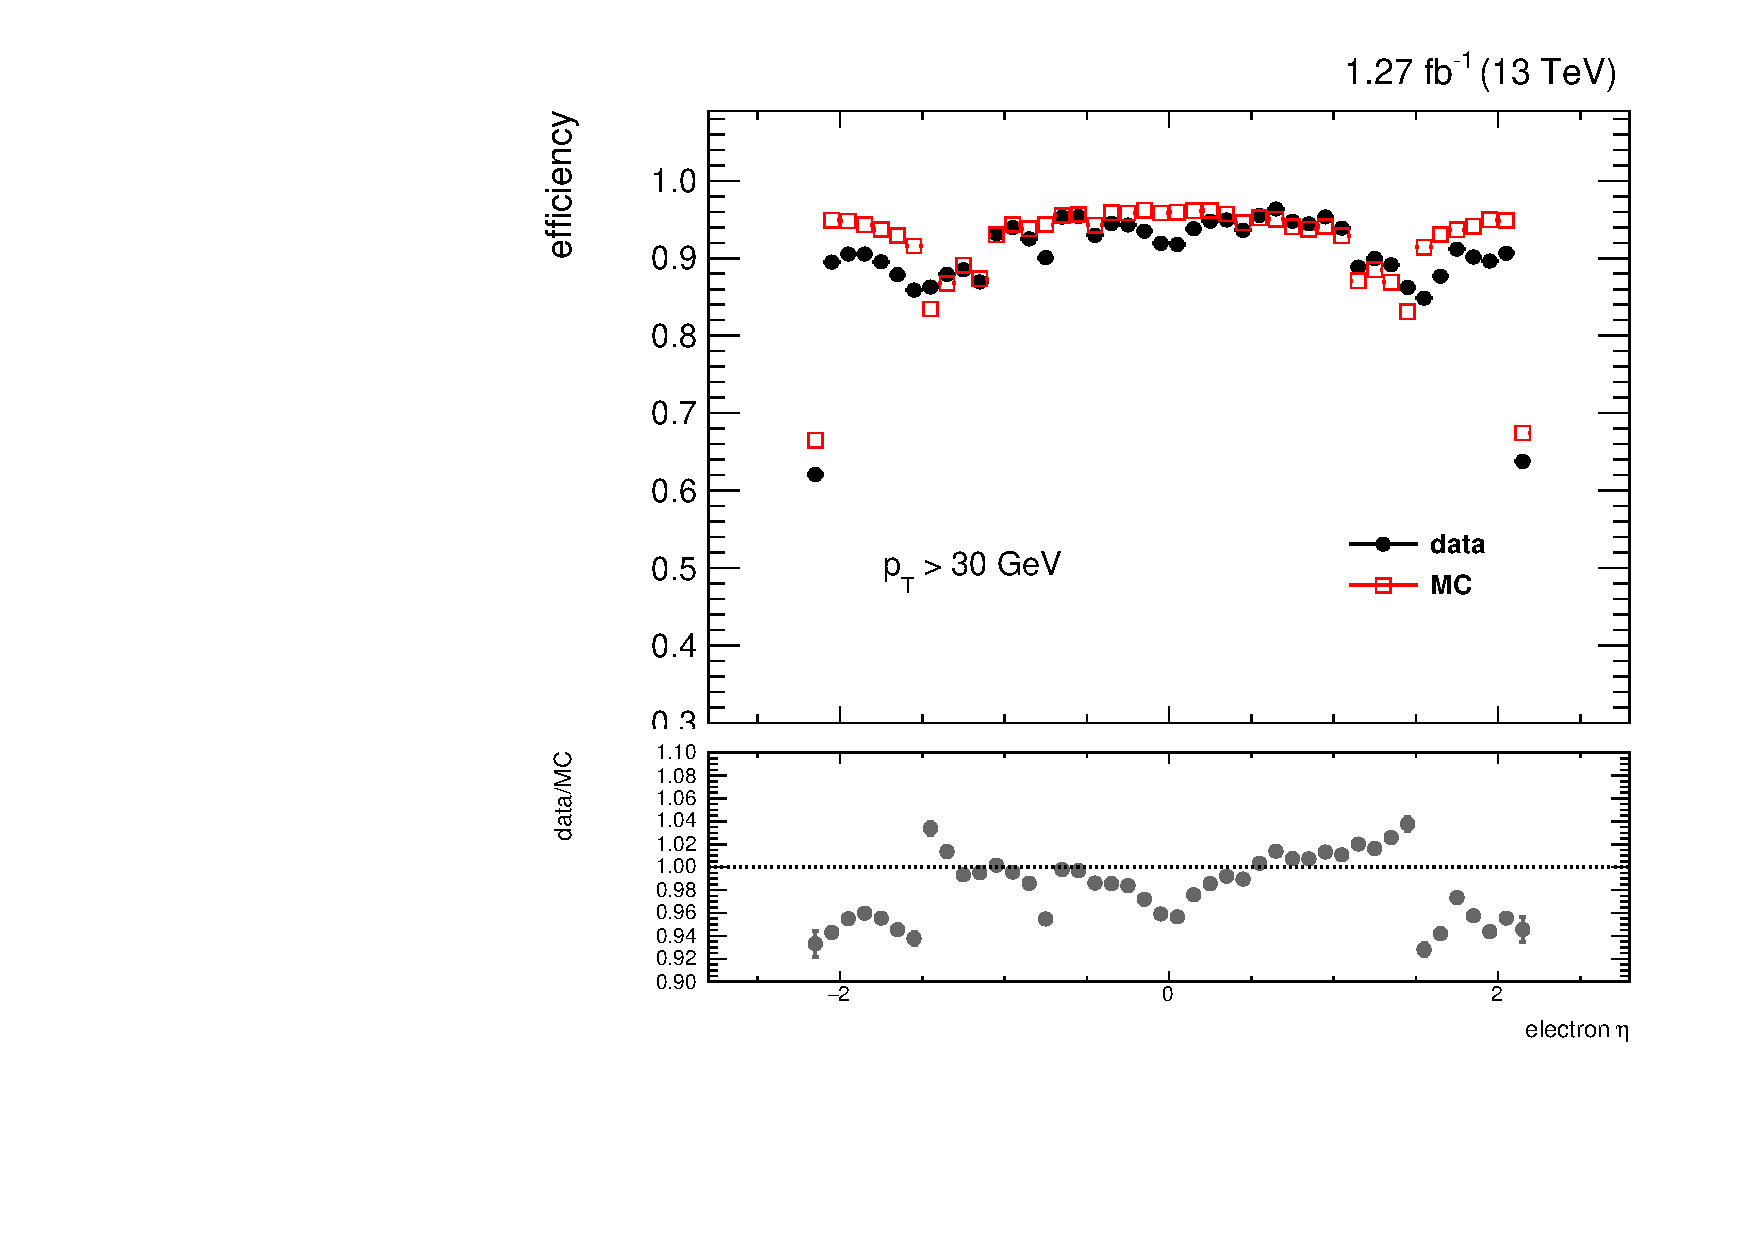
\includegraphics[width=0.48\textwidth]{figures/sel_effeta_dataMC.pdf}
  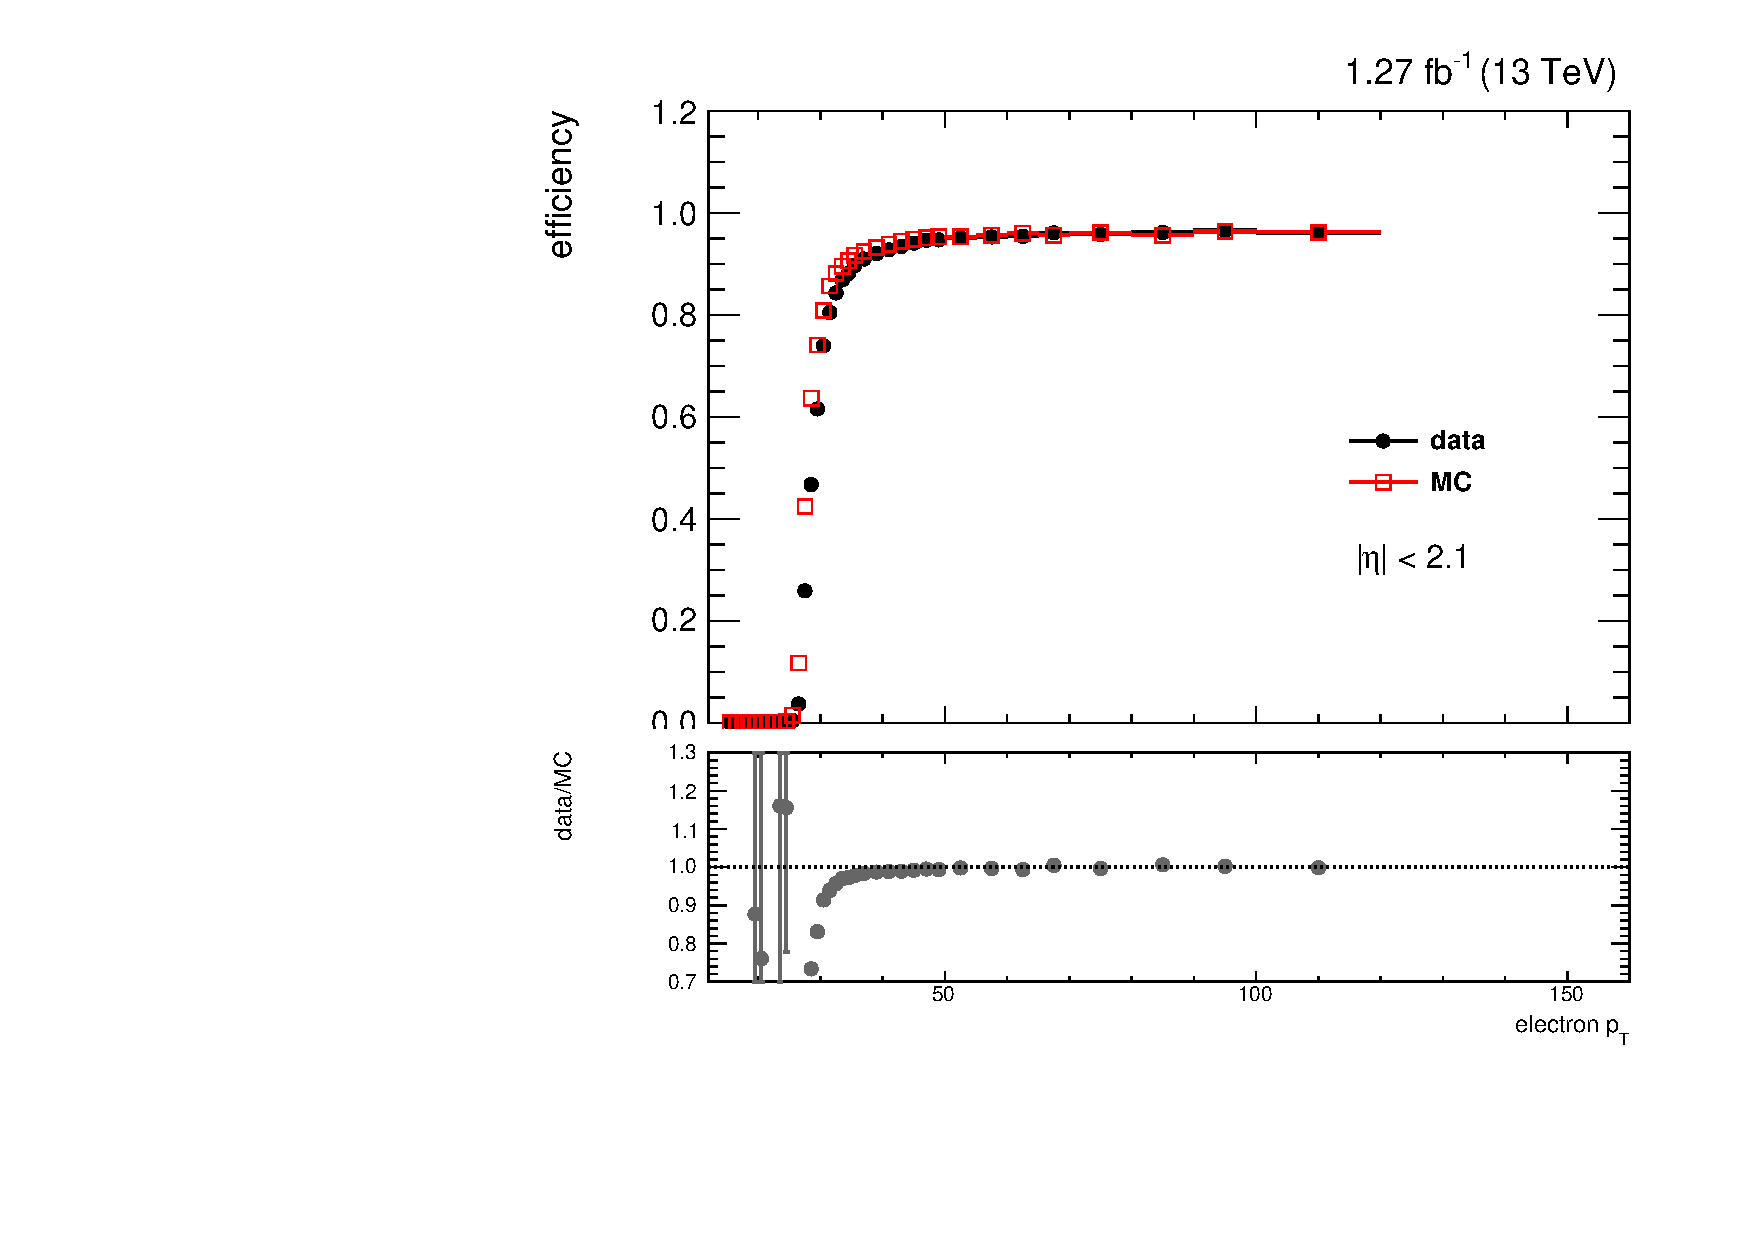
\includegraphics[width=0.48\textwidth]{figures/sel_effpt_dataMC.pdf}
  \caption{Efficiency of HLT\_Ele27\_eta2p1\_WP75\_Gsf in MC and HLT\_Ele27\_eta2p1\_WPLoose\_Gsf in data with respect to $\eta$ (left) and $\pt$ for $|\eta|<2.1$ (right).}
  \label{fig:seleff}
\end{figure}

\begin{figure}[htbp]
  \centering
  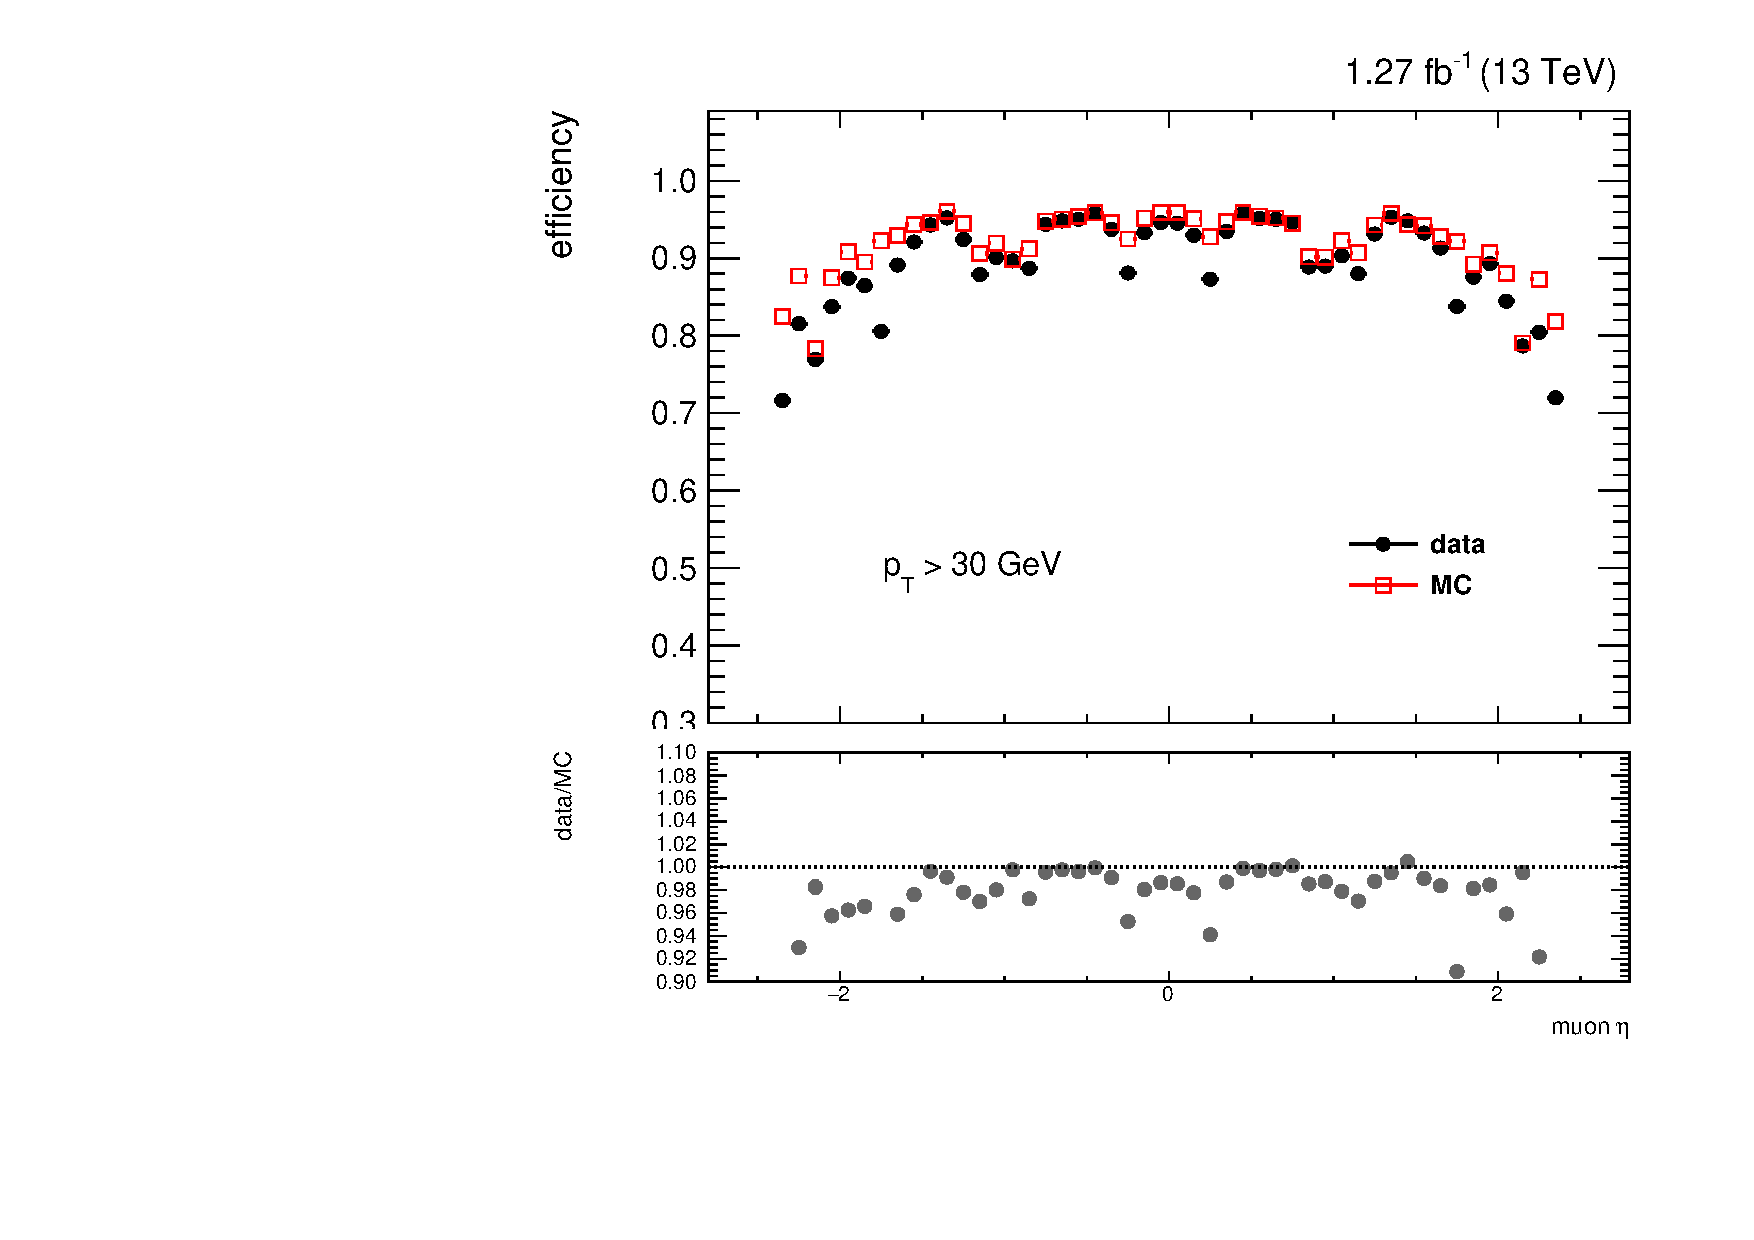
\includegraphics[width=0.48\textwidth]{figures/smu_effeta_dataMC.pdf}
  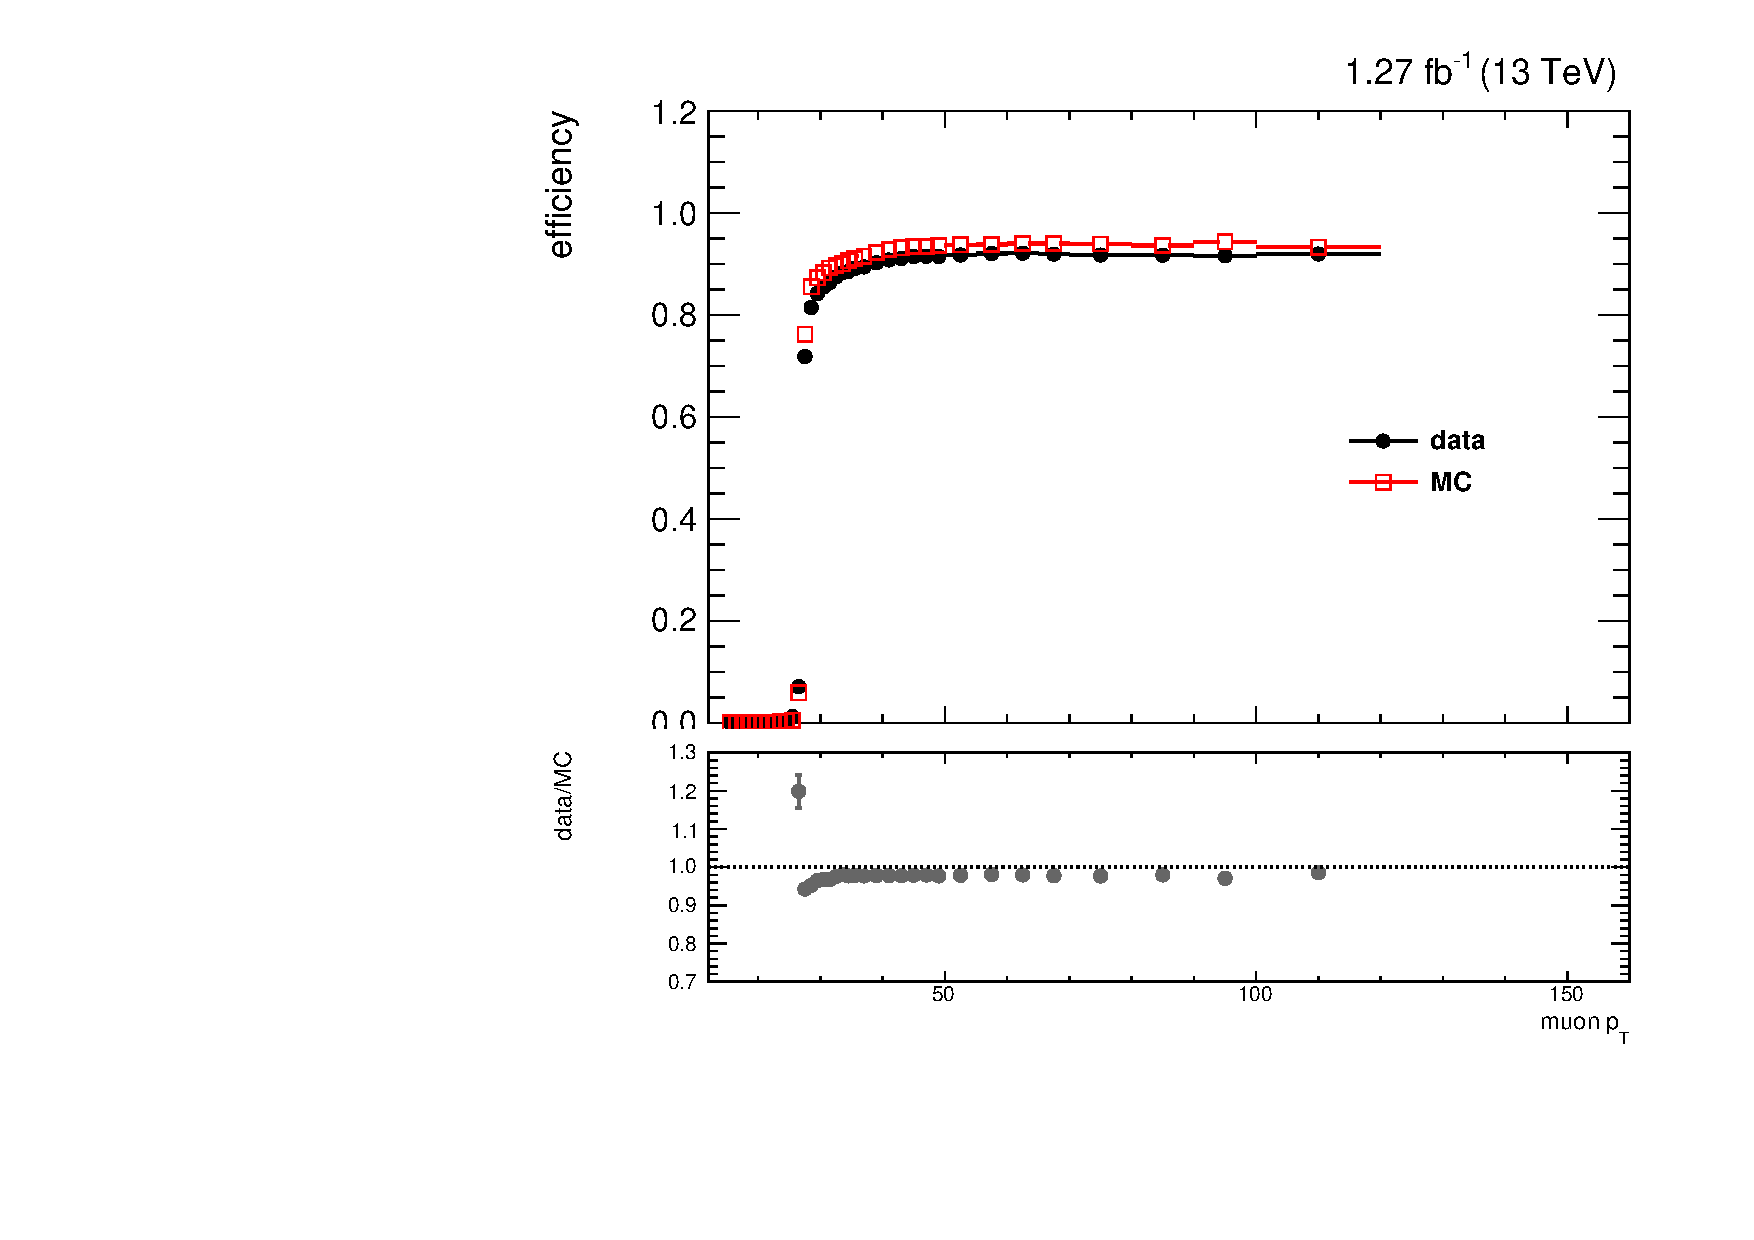
\includegraphics[width=0.48\textwidth]{figures/smu_effpt_dataMC.pdf}
  \caption{Efficiency of HLT\_IsoMu27 in data and MC with respect to $\eta$ (left) and $\pt$ for $|\eta|<2.4$ (right).}
  \label{fig:smueff}
\end{figure}

\clearpage

In order to greatly reduce semileptonic $\ttbar$ and $\Wjets$ background, events are required to have high transverse mass, $M_T$, defined as,
\begin{equation}
M_T = \sqrt{2\,\pt^{\Lep}\,\met \left(1-\cos\Delta\phi_{\Lep,\met}\right)}.
\end{equation}

The remaining $\ttbar$ background is predominantly from the dilepton channel. Two variables that help reject this background are $M_{T2}^W$ and $\min_{i=1,2}\Delta\phi\left(j_i,\met\right)$, the minimum $\Delta\phi$ between jet and $\met$ among the two leading jets. The offline event selection is,
\begin{itemize}
\item $\met > 160\:\GeV$,
\item exactly one electron or muon passing ``Tight'' selection with $\pt>30\:\GeV$ and $|\eta|<2.1$ and matched to the trigger object,
\item at least $3$ AK4CHS jets with $\pt>30\:\GeV$ and $|\eta|<4$,
  \begin{itemize}
  \item at least one of which has $|\eta|<2.4$ and $\Bot$-tagged,
  \end{itemize}
\item no additional muons passing ``Loose'' selection with $\pt>10\:\GeV$ and $|\eta|<2.4$,
\item no additional electrons passing ``Veto'' selection with $\pt>10\:\GeV$ and $|\eta|<2.5$,
\item $M_T > 160\:\GeV$,
\item $M_{T2}^W > 200\:\GeV$,
\item $\min_{i=1,2}\Delta\phi\left(j_i,\met\right)>1.2$.
\end{itemize}

\begin{figure}[htbp]
  \centering
  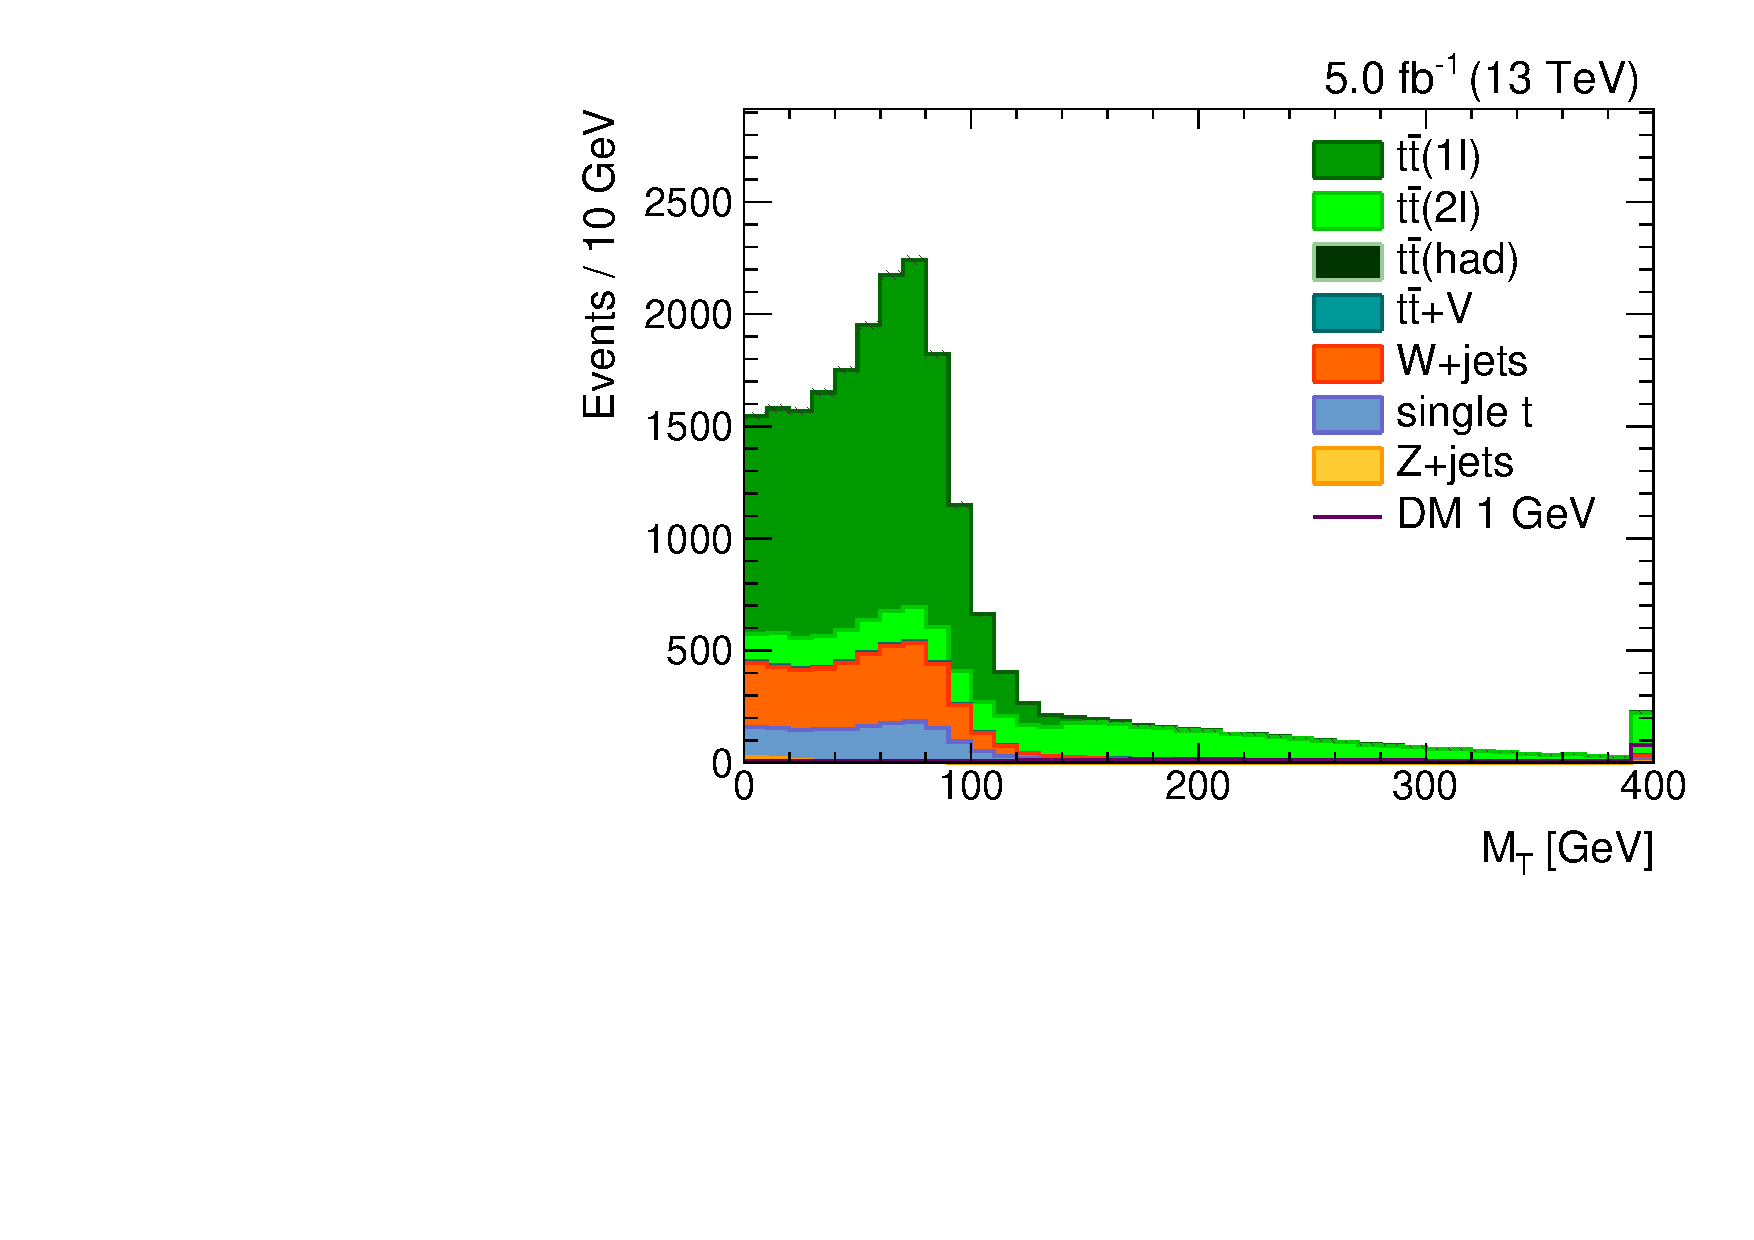
\includegraphics[width=0.48\textwidth]{figures/semilept-incl-mt_l.pdf}
  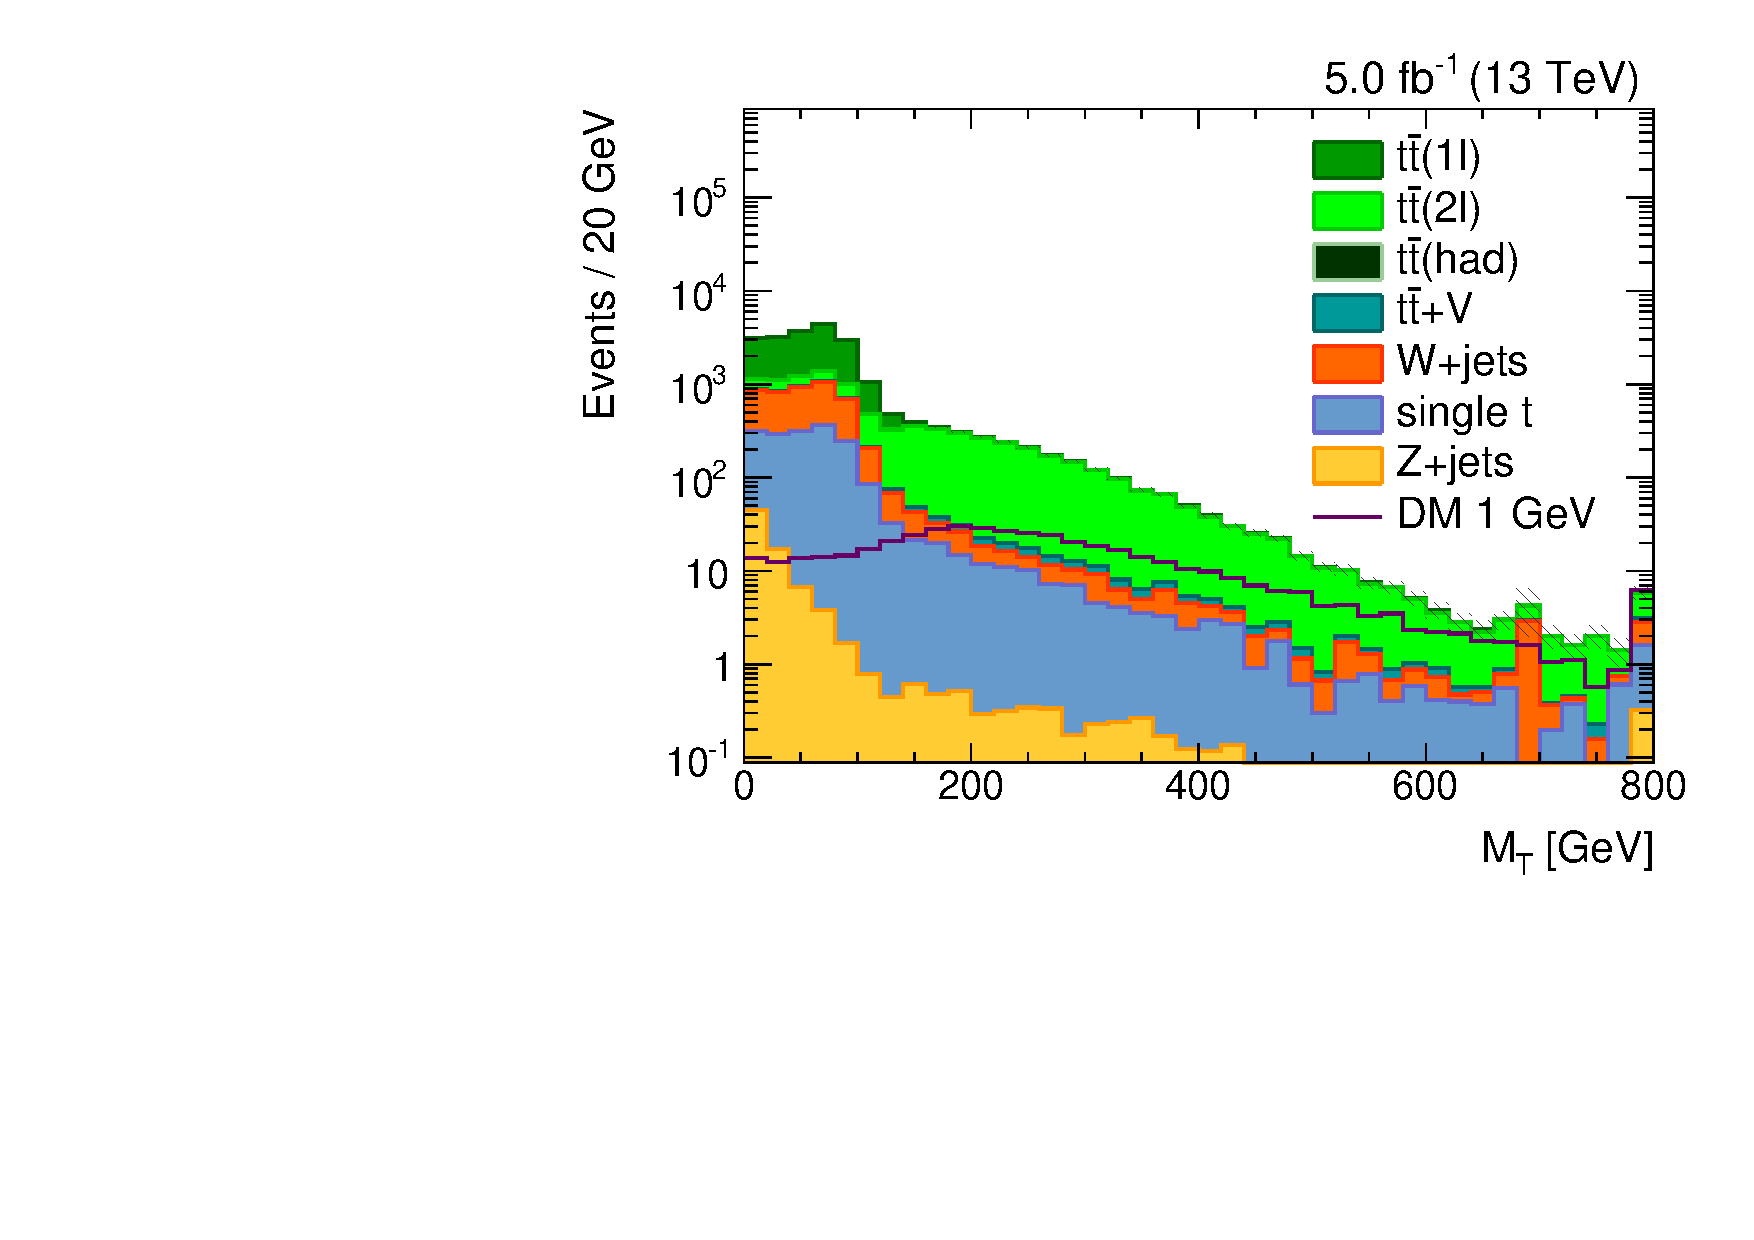
\includegraphics[width=0.48\textwidth]{figures/semilept-incl-mtlog_l.pdf}
  \caption{The $M_T$ distribution in linear (left) and log (right) scales. Note that the right-most bin includes overflow.}
  \label{fig:incl_semilept_mt}
\end{figure}

\begin{figure}[htbp]
  \centering
  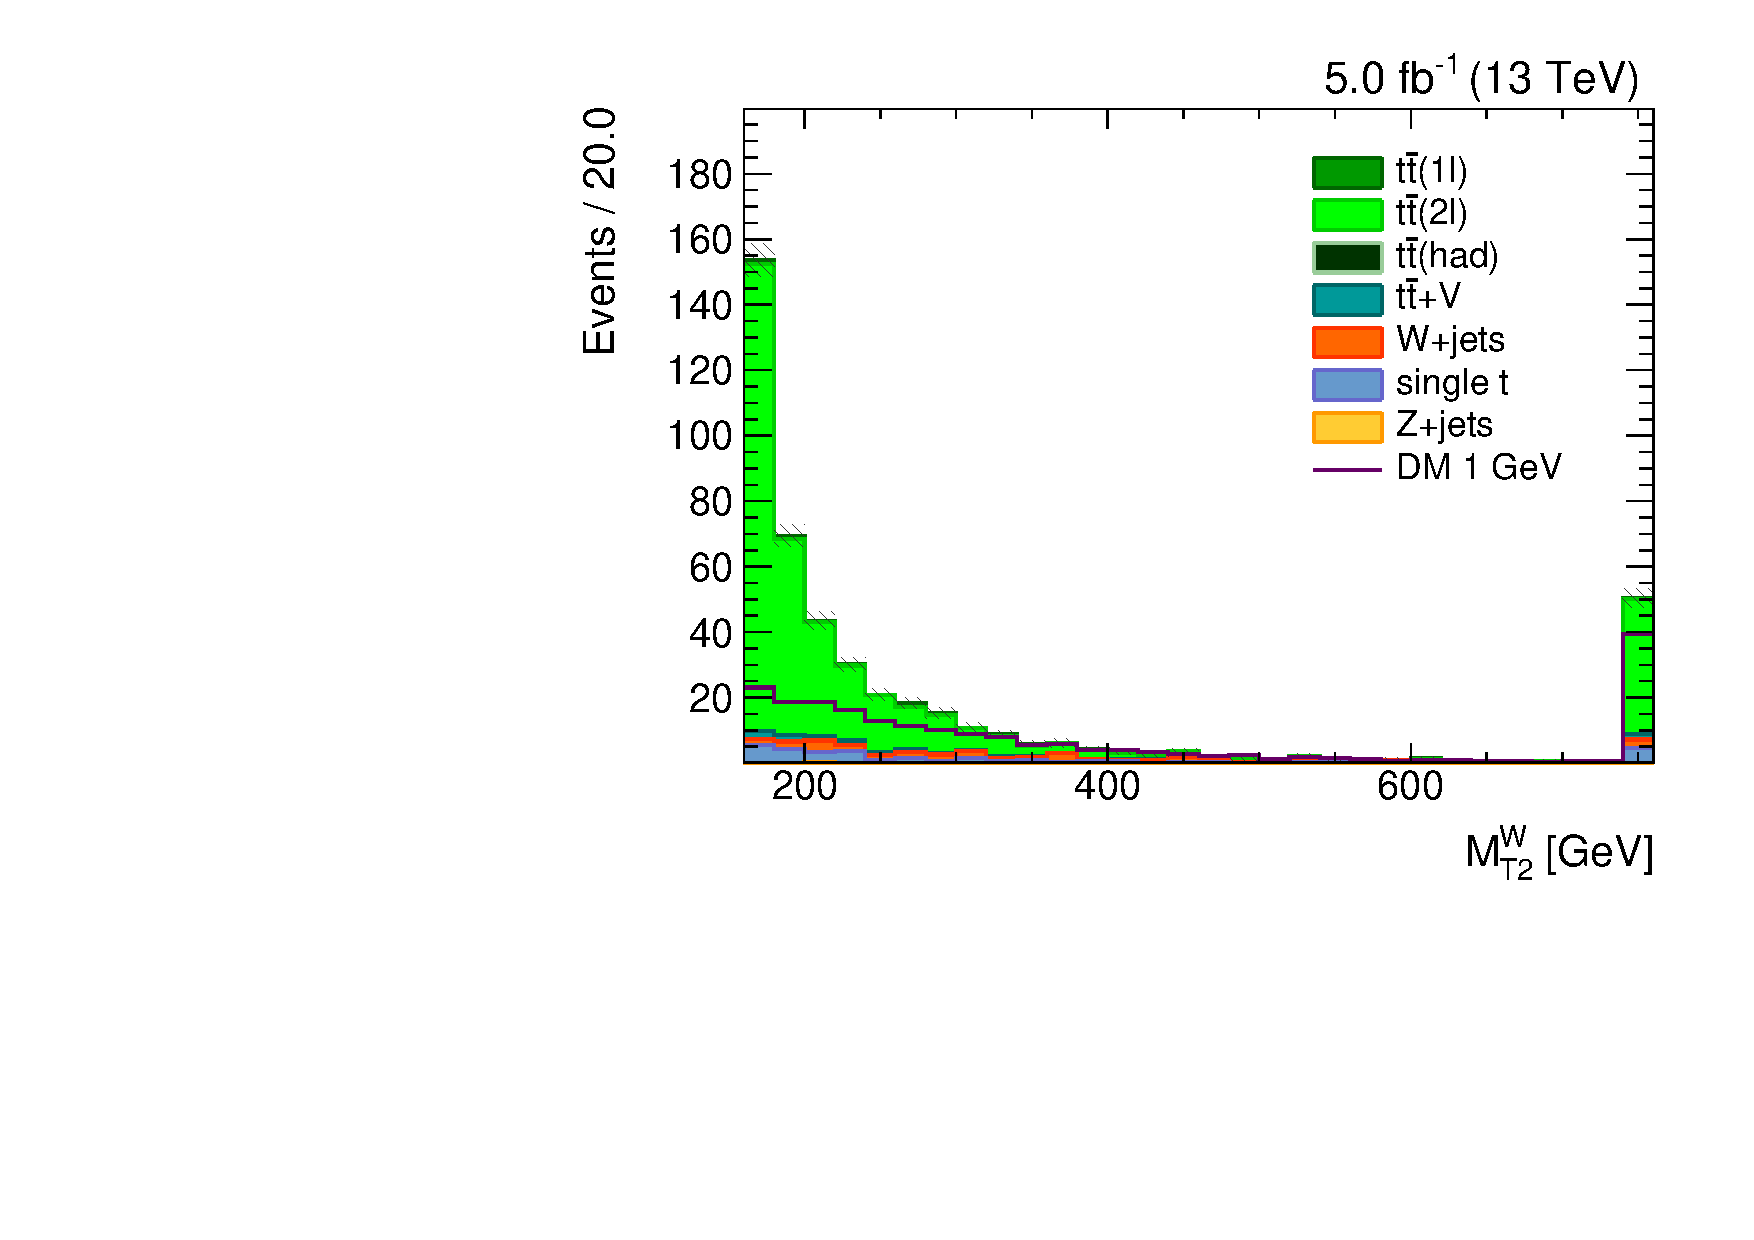
\includegraphics[width=0.48\textwidth]{figures/semilept-incl-mt2w_l.pdf}
  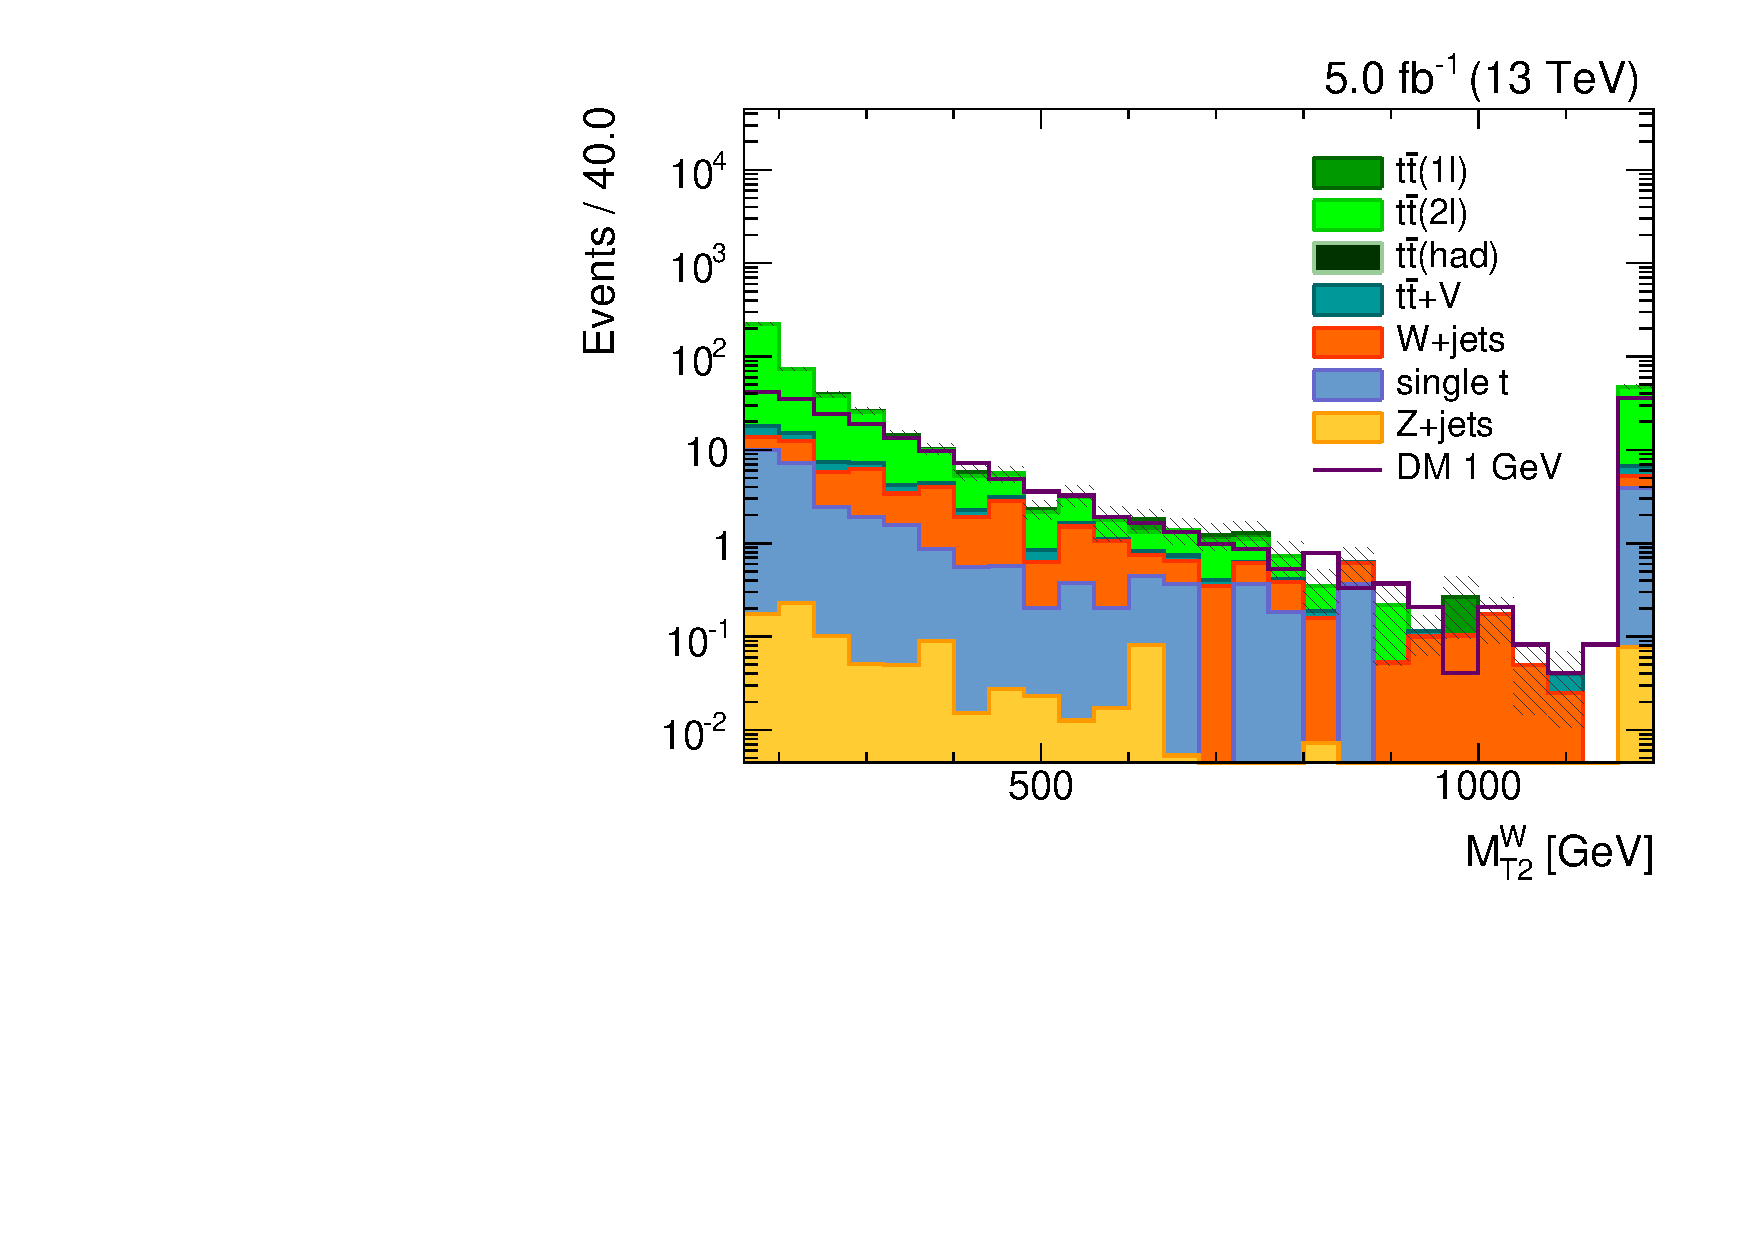
\includegraphics[width=0.48\textwidth]{figures/semilept-incl-mt2wlog_l.pdf}
  \caption{The $M_{T2}^W$ distribution in linear (left) and log (right) scales. Note that the right-most bin includes overflow.}
  \label{fig:incl_semilept_mt2w}
\end{figure}

\begin{figure}[htbp]
  \centering
  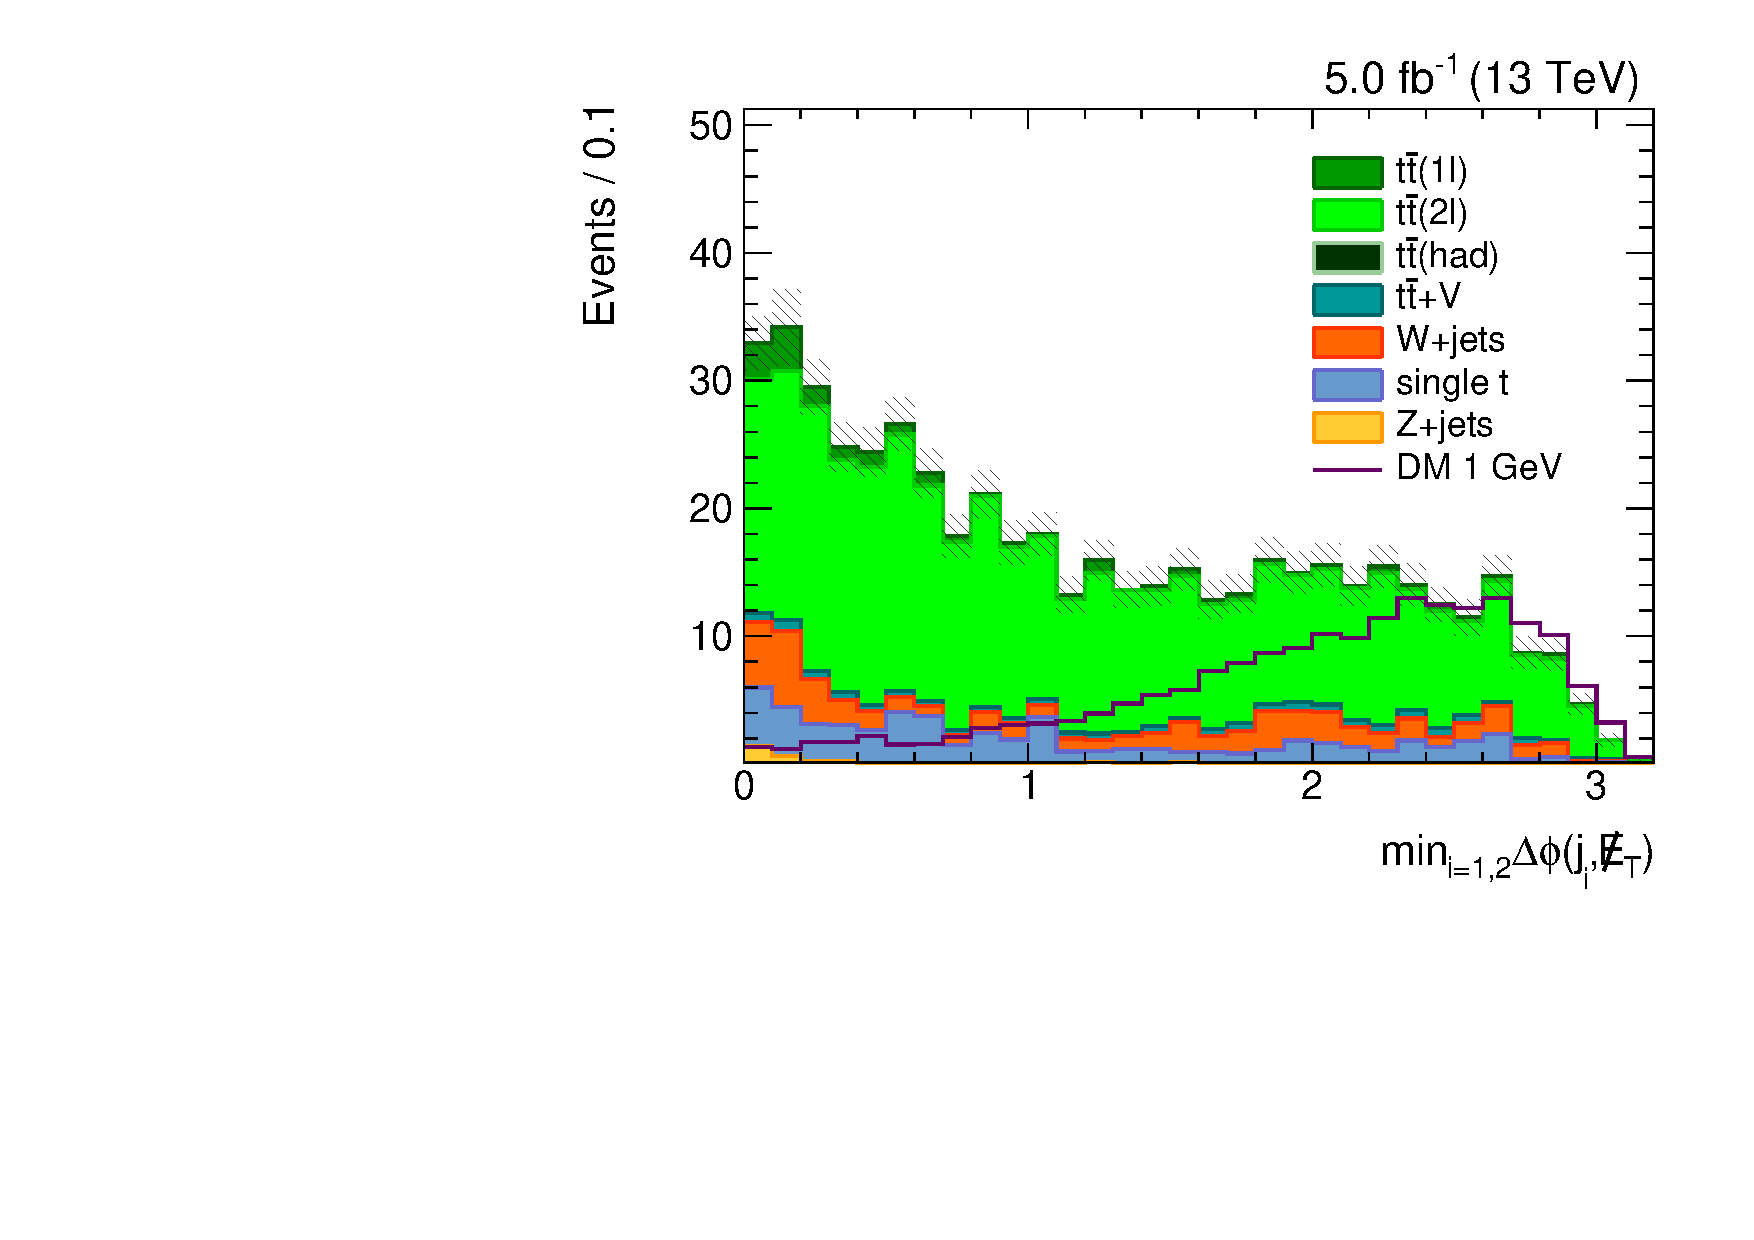
\includegraphics[width=0.48\textwidth]{figures/semilept-incl-dphijetmet2_l.pdf}
  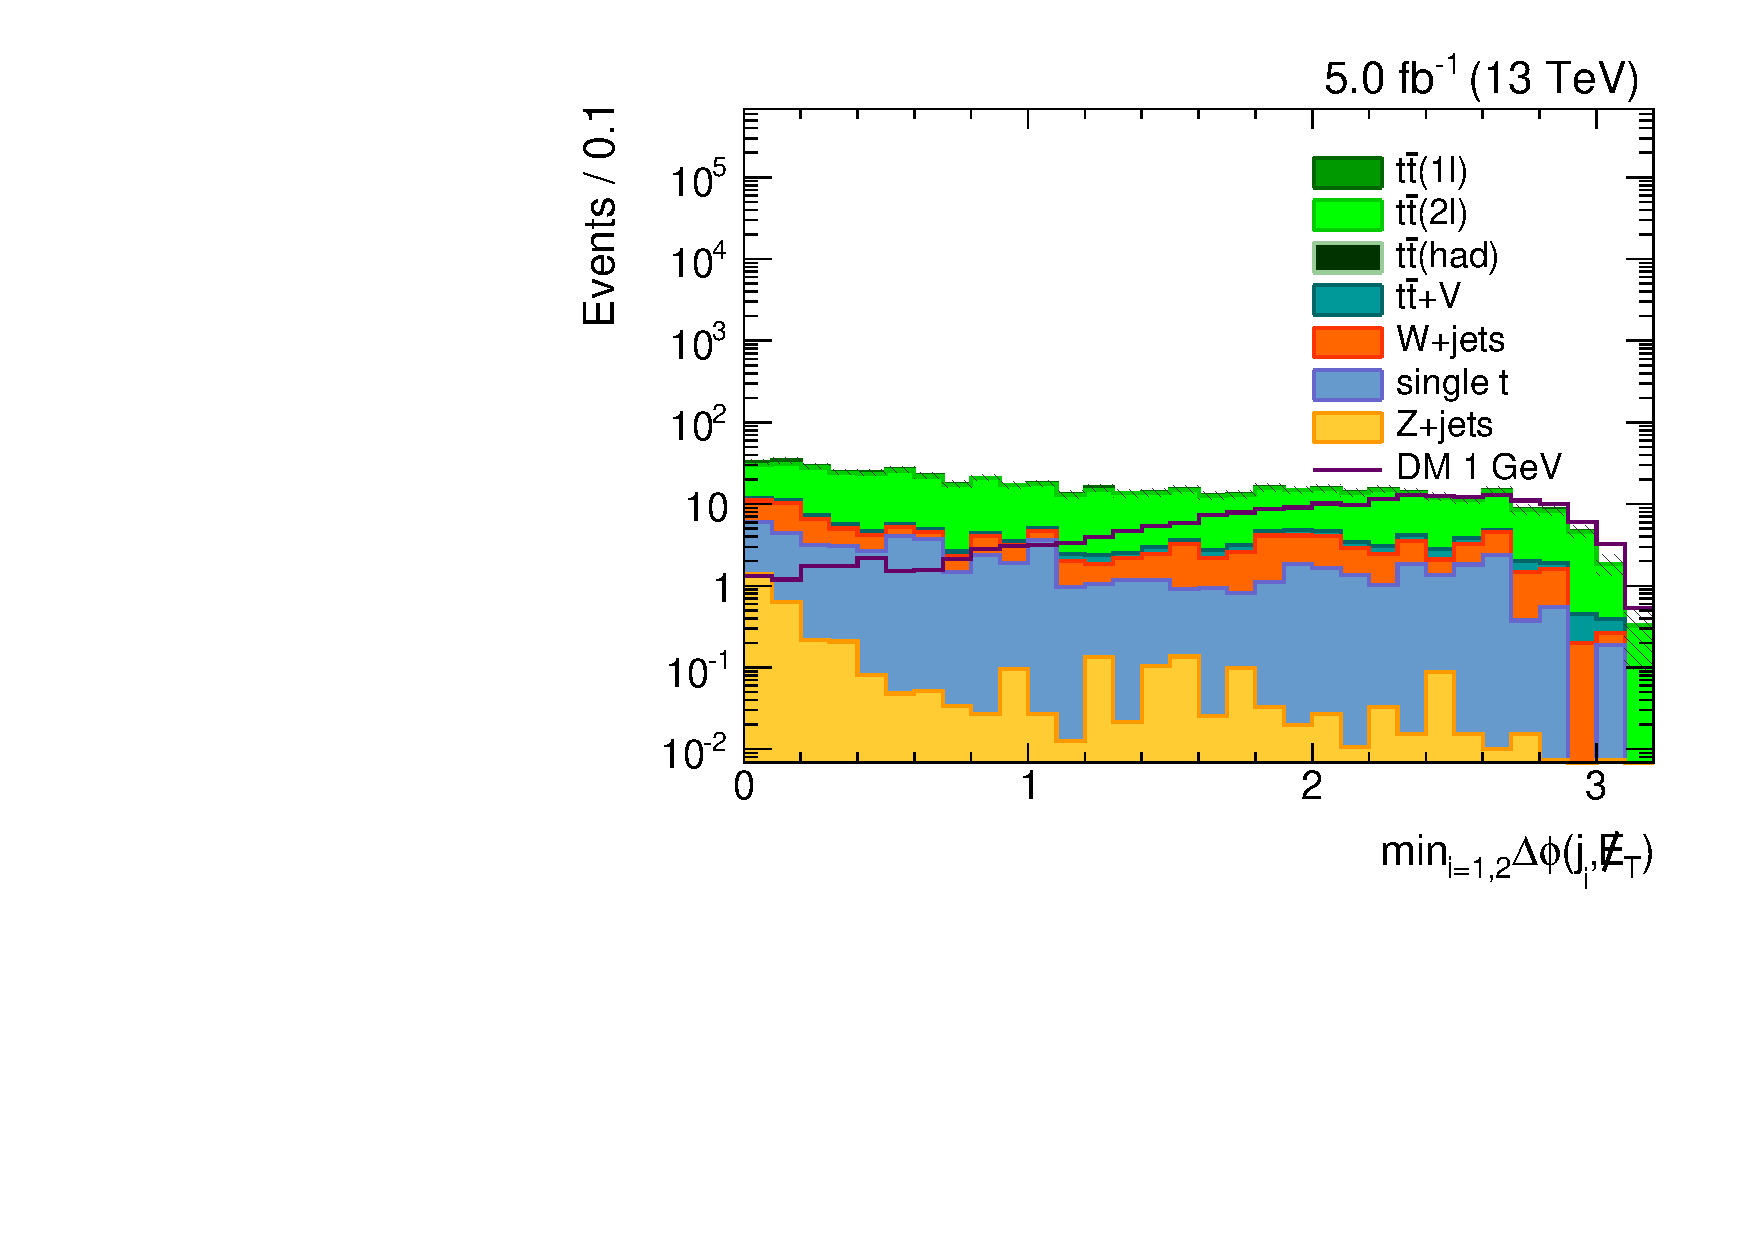
\includegraphics[width=0.48\textwidth]{figures/semilept-incl-dphijetmet2log_l.pdf}
  \caption{The $\min_{i=1,2}\Delta\phi\left(j_i\,\met\right)$ distribution in linear (left) and log (right) scales.}
  \label{fig:incl_semilept_dphijetmet2}
\end{figure}

The $\met$ distribution after selection is shown in Fig.~\ref{fig:incl_semilept_met}.
\begin{figure}[htbp]
  \centering
  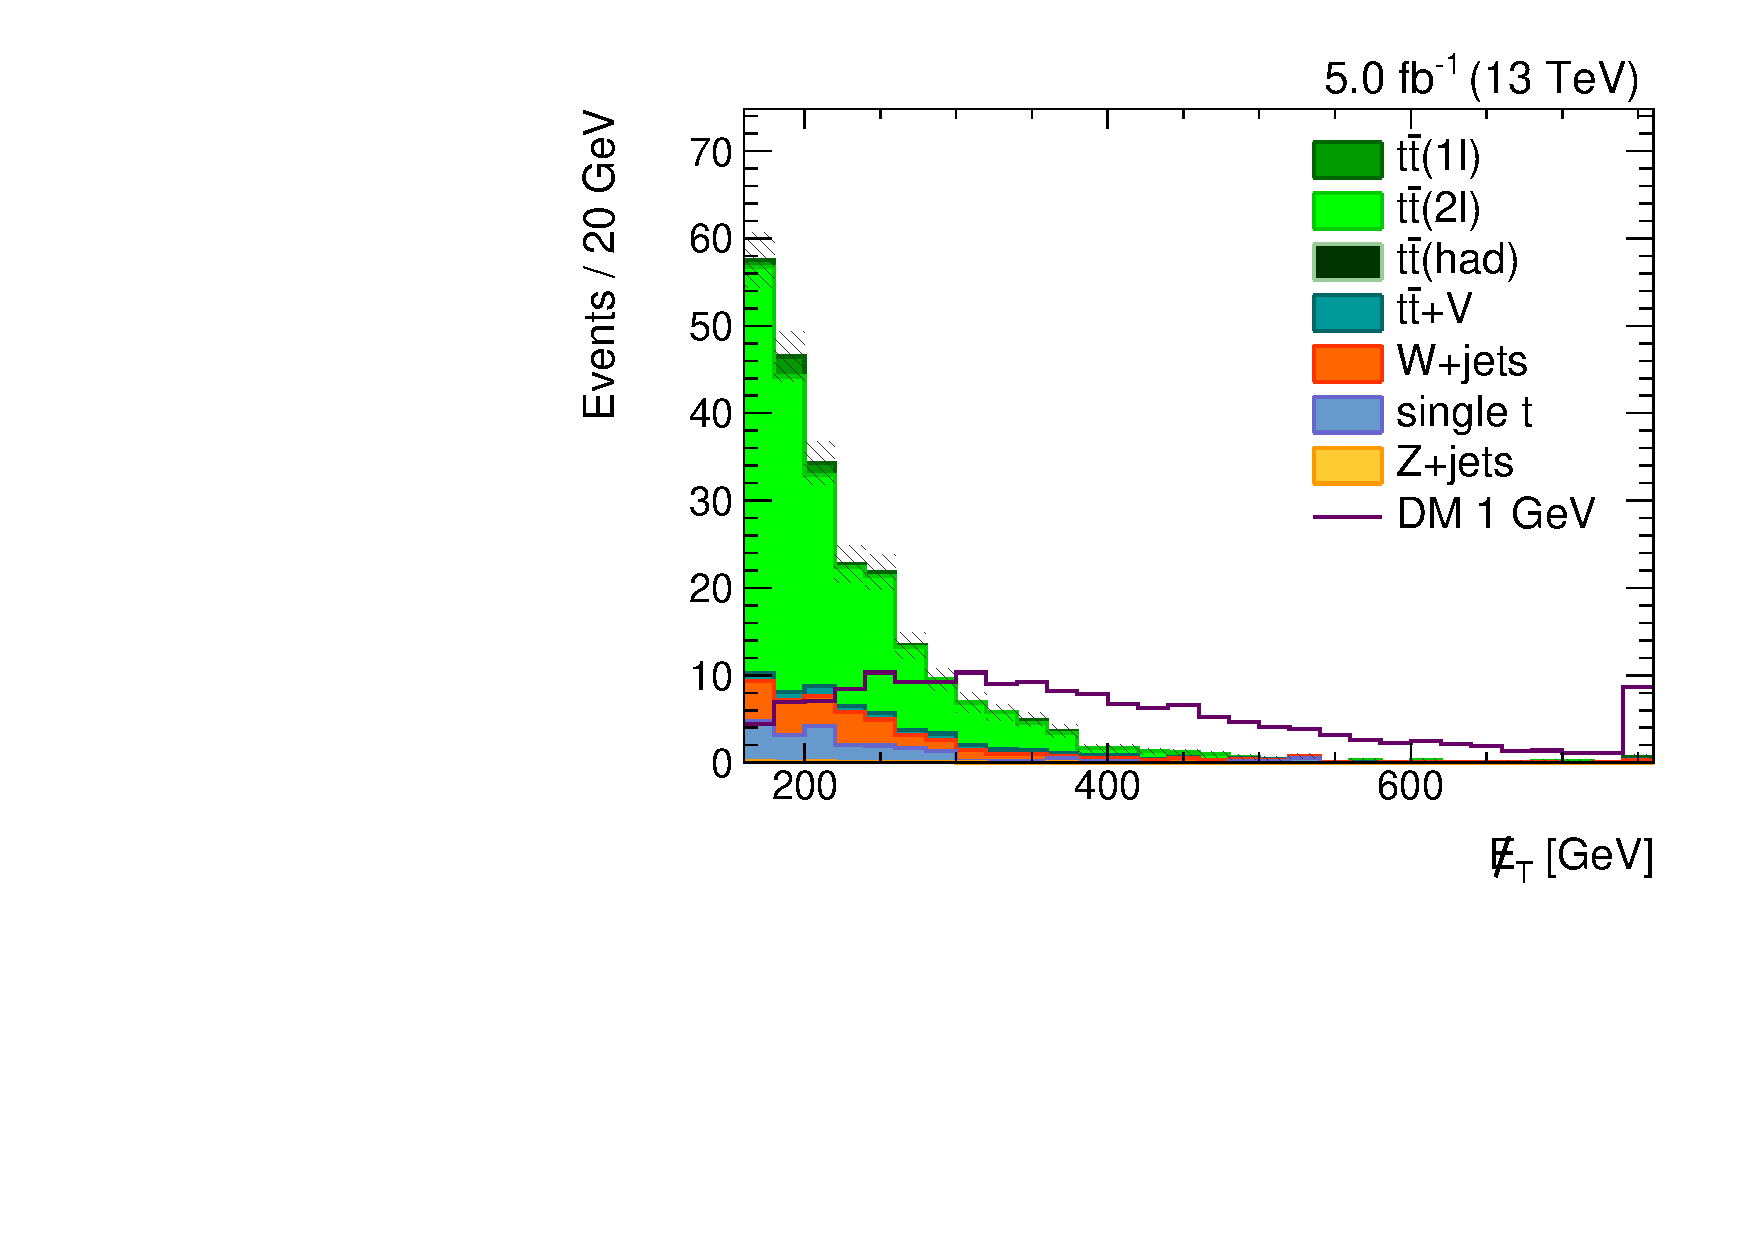
\includegraphics[width=0.48\textwidth]{figures/semilept-incl-met_l.pdf}
  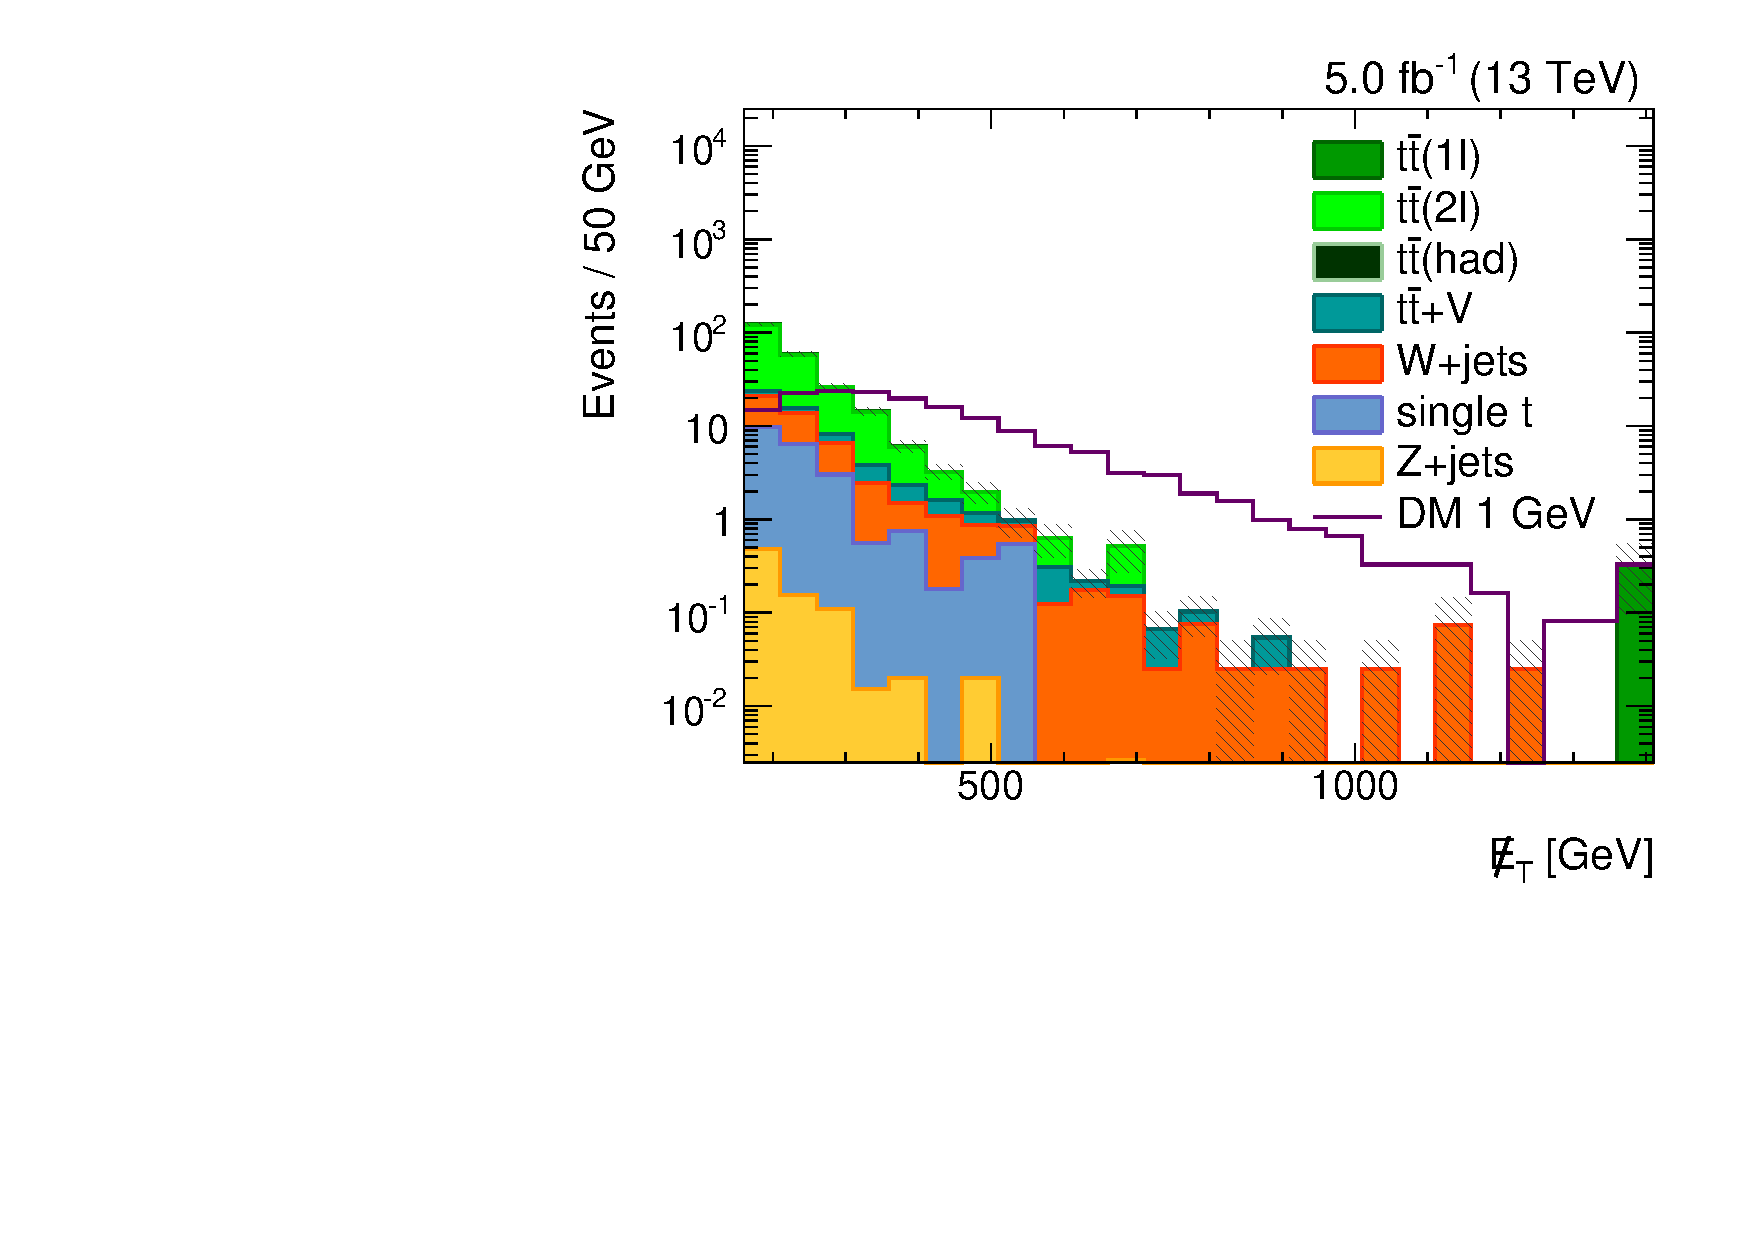
\includegraphics[width=0.48\textwidth]{figures/semilept-incl-metlog_l.pdf}
  \caption{The $\met$ distribution after semileptonic selection in linear (left) and log (right) scales. Note that the right-most bin includes overflow.}
  \label{fig:incl_semilept_met}
\end{figure}

The expected yields for $5\:\ifb$ after selection are shown in Table~\ref{tab:incl_semilept_yields}.

\begin{table}[!ht]
\centering
\begin{tabular}{|c|rr|r|}
\hline
  Process & \multicolumn{1}{|c}{$e$} & \multicolumn{1}{c|}{$\mu$} & \multicolumn{1}{|c|}{$e+\mu$} \\
\hline
  \Z\To\Lep\Lep         & $  0.28 \pm 0.09$ & $  0.52 \pm 0.14$ & $  0.80 \pm 0.17$ \\
  Single \Top           & $  7.75 \pm 1.18$ & $ 13.01 \pm 1.53$ & $ 20.76 \pm 1.93$ \\
  \Wjets                & $ 11.23 \pm 1.57$ & $ 16.31 \pm 2.35$ & $ 27.54 \pm 2.83$ \\
  $\ttbar+V$            & $  4.22 \pm 0.24$ & $  5.27 \pm 0.27$ & $  9.50 \pm 0.37$ \\
  $\ttbar\mbox{(had)}$  & $  0.00 \pm 0.00$ & $  0.00 \pm 0.00$ & $  0.00 \pm 0.00$ \\
  $\ttbar(2\Lep)$       & $ 77.30 \pm 3.55$ & $ 95.61 \pm 3.95$ & $172.91 \pm 5.32$ \\
  $\ttbar(1\Lep)$       & $  3.43 \pm 0.75$ & $  2.78 \pm 0.67$ & $  6.21 \pm 1.01$ \\

\hline
  SM expected           & $365.94 \pm 4.14$ & $133.50 \pm 4.91$ & $237.72 \pm 6.42$ \\
\hline
  $M_\chi=1\:\GeV$      & $289.61 \pm 1.75$ & $ 91.77 \pm 1.94$ & $165.93 \pm 2.61$ \\
\hline
\end{tabular}
\caption{Expected yields for $5\:\ifb$ after the inclusive selection for the semileptonic channel.}
\label{tab:incl_semilept_yields}
\end{table}

%\subsection{Boosted Top Tagging}
\label{subsec:sel_toptag_boosted}

Jet substructure techniques can be used to identify boosted top decays where all the decay products are contained within a single jet. Wider jets are considered so that substructure methods are applicable for tops with moderate boost. In this analysis, jets with $R=1.5$ are considered so that tops with $\pt>250\:\GeV$ are fairly well contained within the jet. Soft drop jet grooming, $N$-subjettiness, and subjet $\Bot$-tagging are applied to tag top decays.

By analyzing the radiation pattern within a jet, it is possible to differentiate between a jet induced by a single parton and a jet induced by the decay of a massive particle. The soft drop algorithm removes soft, wide angled radiation and decomposes a jet into subjets that correspond to the underlying hard partons that induce the jet. The settings used for soft drop are $\beta=0$ and $z_{\mbox{\scriptsize{cut}}}=0.1$. The soft drop mass ($M_{\mbox{\scriptsize{soft drop}}}$) spectrum is shown in Fig.~\ref{fig:softdrop}, for events with a single ``Tight'' muon or electron, $M_T>160\:\GeV$, and at least one AK4CHS $\Bot$-tagged jet.

\begin{figure}[htbp]
  \centering
  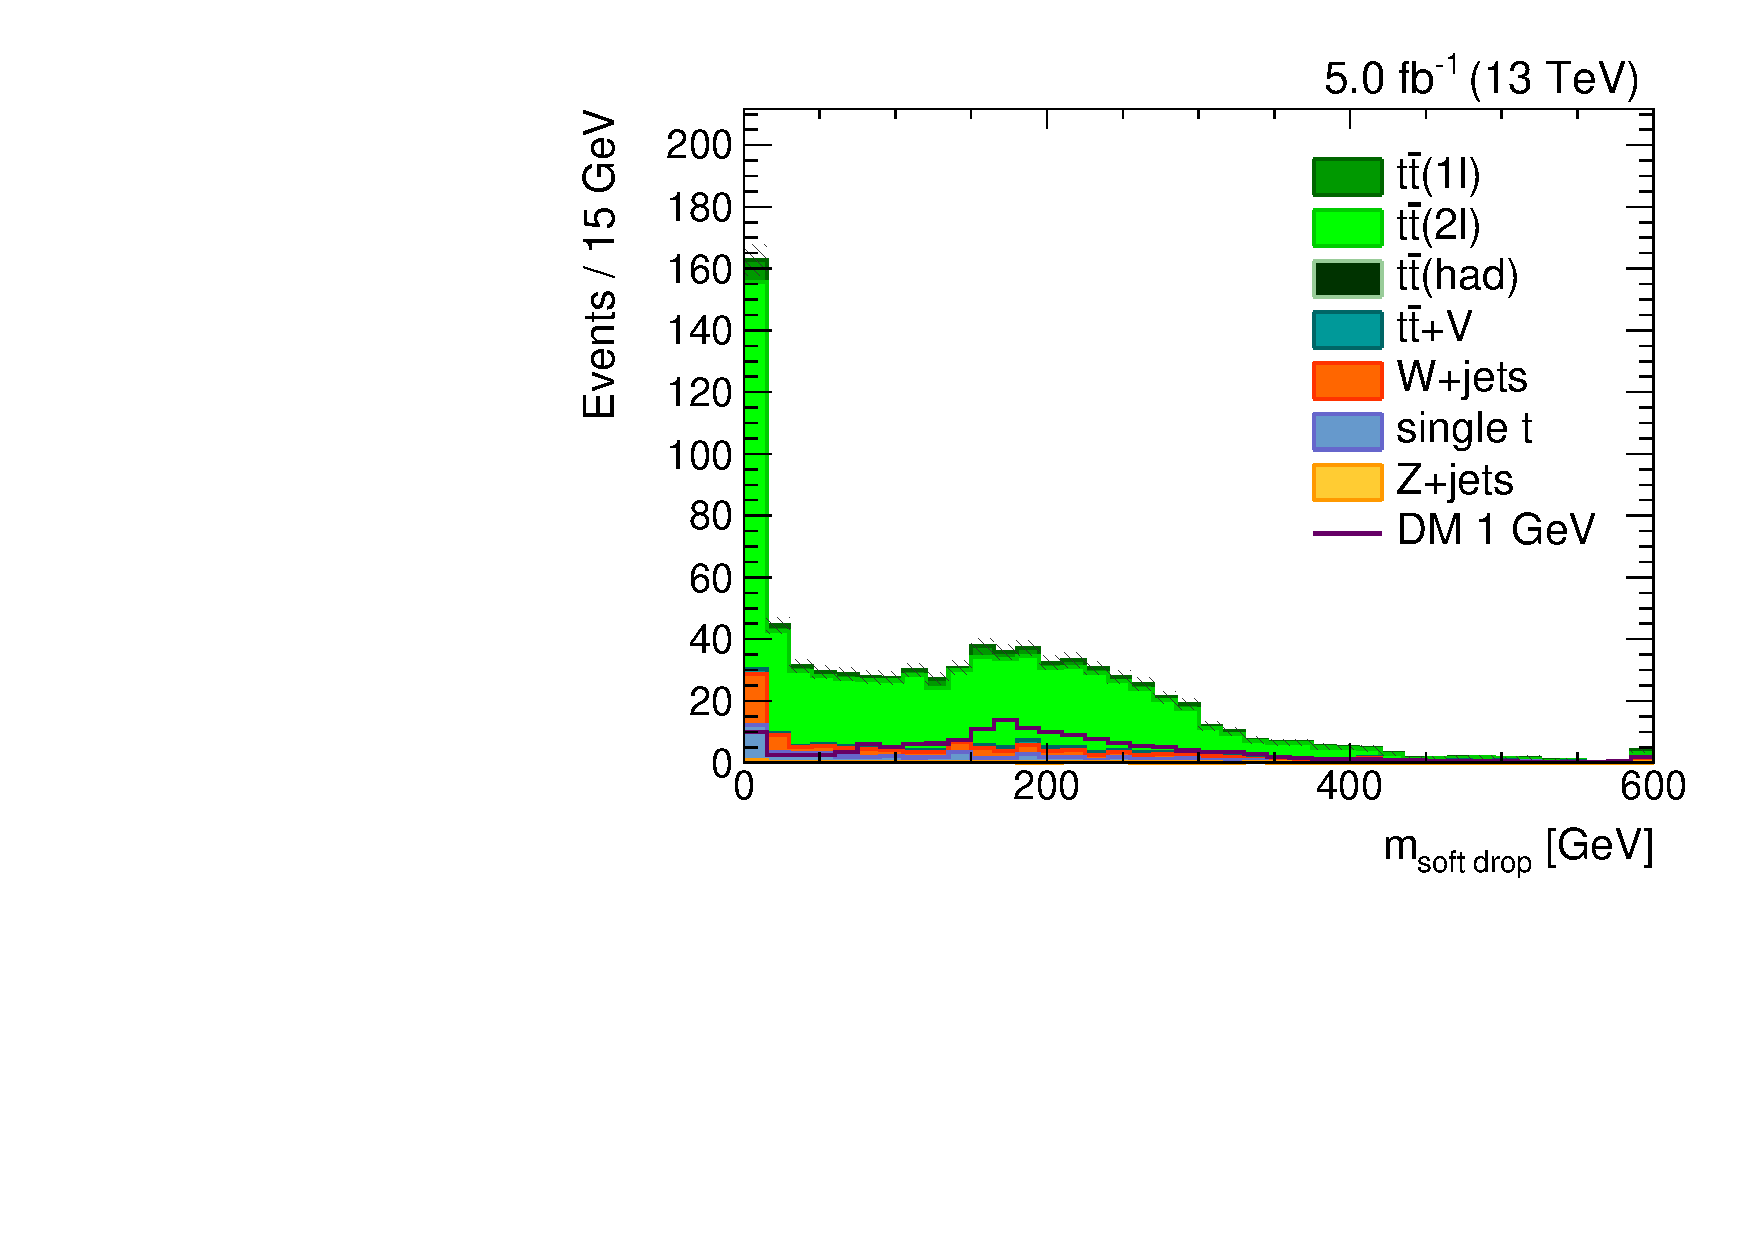
\includegraphics[width=0.48\textwidth]{figures/softdrop.pdf}
  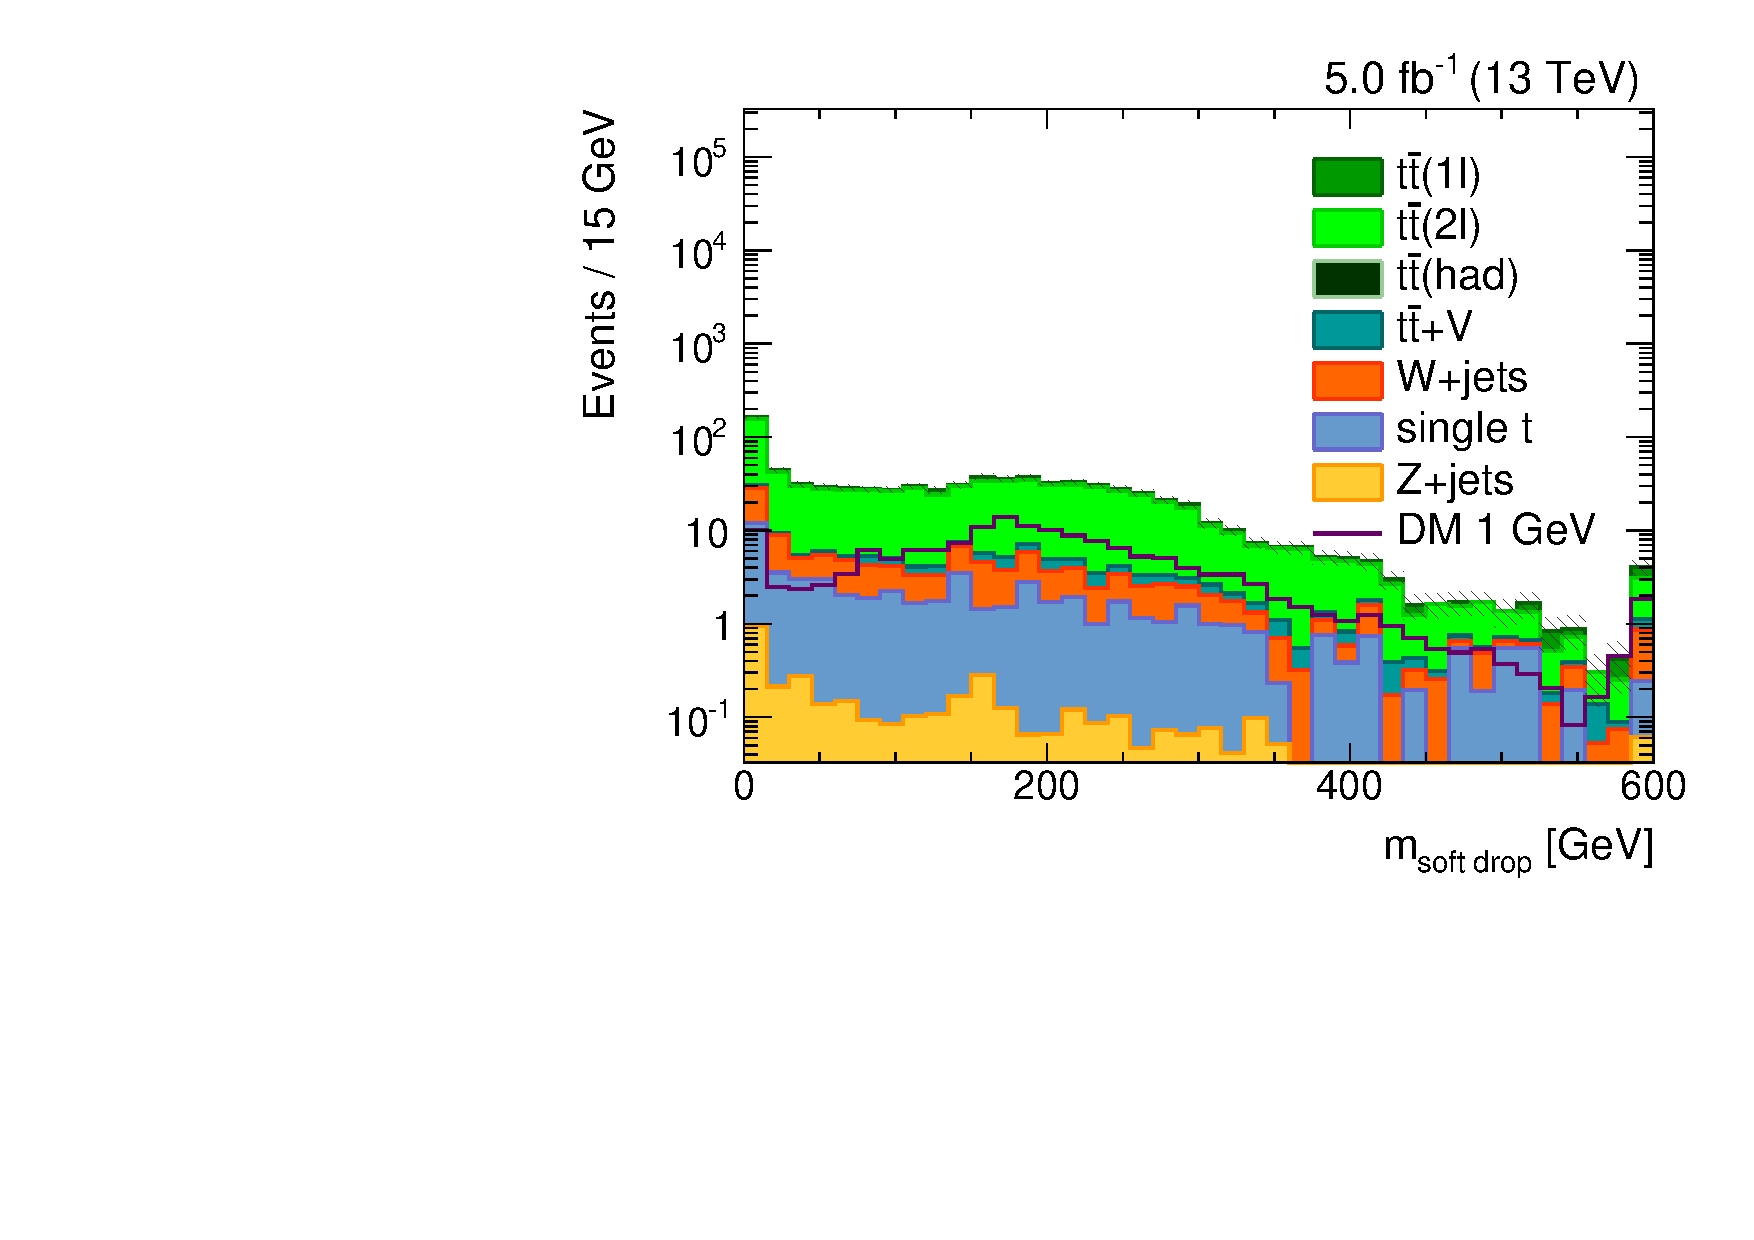
\includegraphics[width=0.48\textwidth]{figures/softdroplog.pdf}
  \caption{Jet mass distribution after grooming with the soft drop ($\beta=0, z_{\mbox{\scriptsize{cut}}}=0.1$) algorithm.}
  \label{fig:softdrop}
\end{figure}

$N$-subjettiness quantifies the likelihood a jet comprises of $N$ or more prongs. The discriminating variable is the ratio of $N$-subjettiness quantities; in particular, the $\tau_n/\tau_{n-1}$ ratio quantifies the likelihood the jet comprises of $n$ prongs. Hence, $\tau_3/\tau_2$ is used to help identify top decays. The $\tau_3/\tau_2$ distribution for events with $M_{\mbox{\scriptsize{soft drop}}}>75\:\GeV$ is shown in Fig.~\ref{fig:tau32}.

\begin{figure}[htbp]
  \centering
  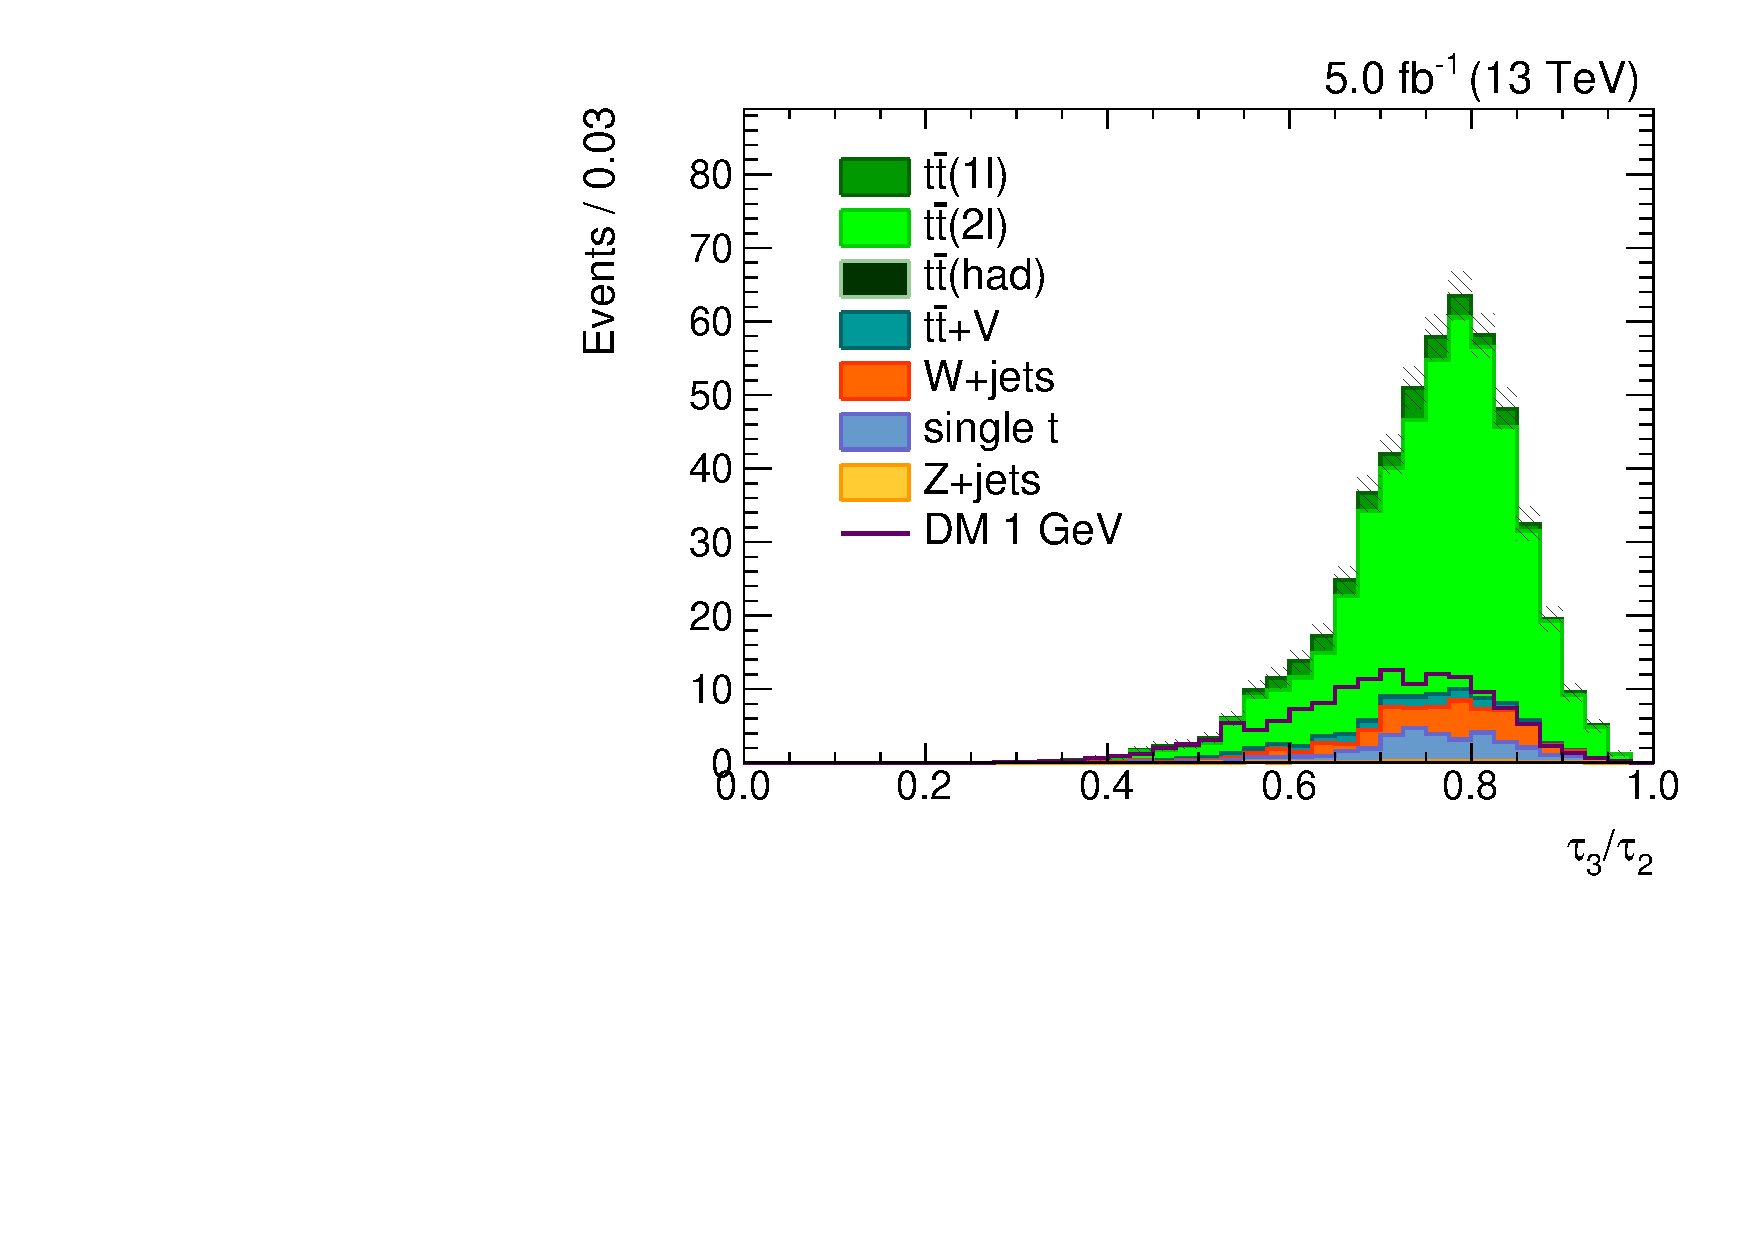
\includegraphics[width=0.48\textwidth]{figures/tau32.pdf}
  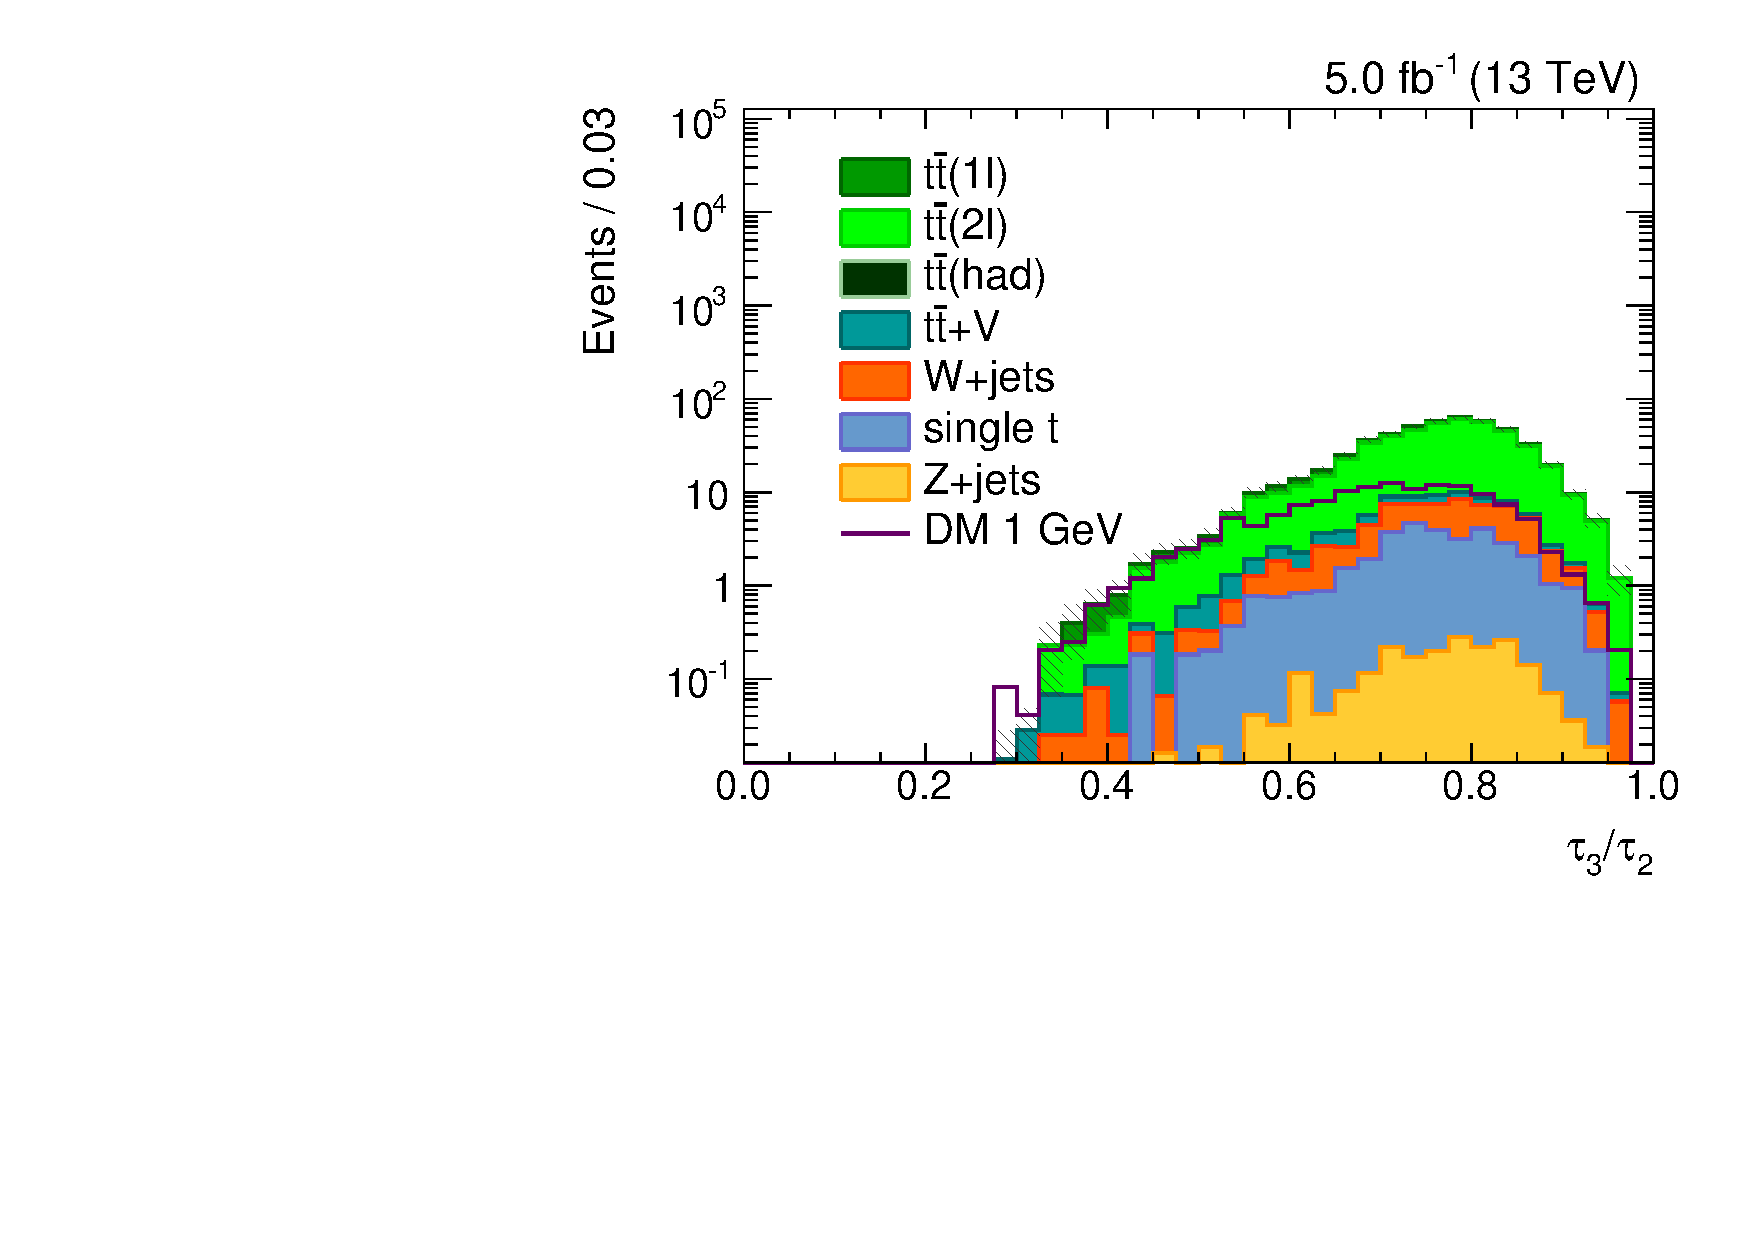
\includegraphics[width=0.48\textwidth]{figures/tau32log.pdf}
  \caption{Distribution of $\tau_3/\tau2$ for jets with $M_{\mbox{\scriptsize{soft drop}}}>75\:\GeV$.}
  \label{fig:tau32}
\end{figure}

The $\Bot$ quark from the top decay is expected to be contained in the wide jet and therefore the corresponding subjet should have properties similar to typical $\Bot$-jets. The CSVv2+IVF $\Bot$-tag algorithm is performed on subjets from the soft drop decomposition to provide further discrimination for top decays. The distribution for the largest $\Bot$-tag value among subjets in a jet, for jets with $M_{\mbox{\scriptsize{soft drop}}}>75\:\GeV$, is shown in Fig.~\ref{fig:subjet_btag}.

\begin{figure}[htbp]
  \centering
  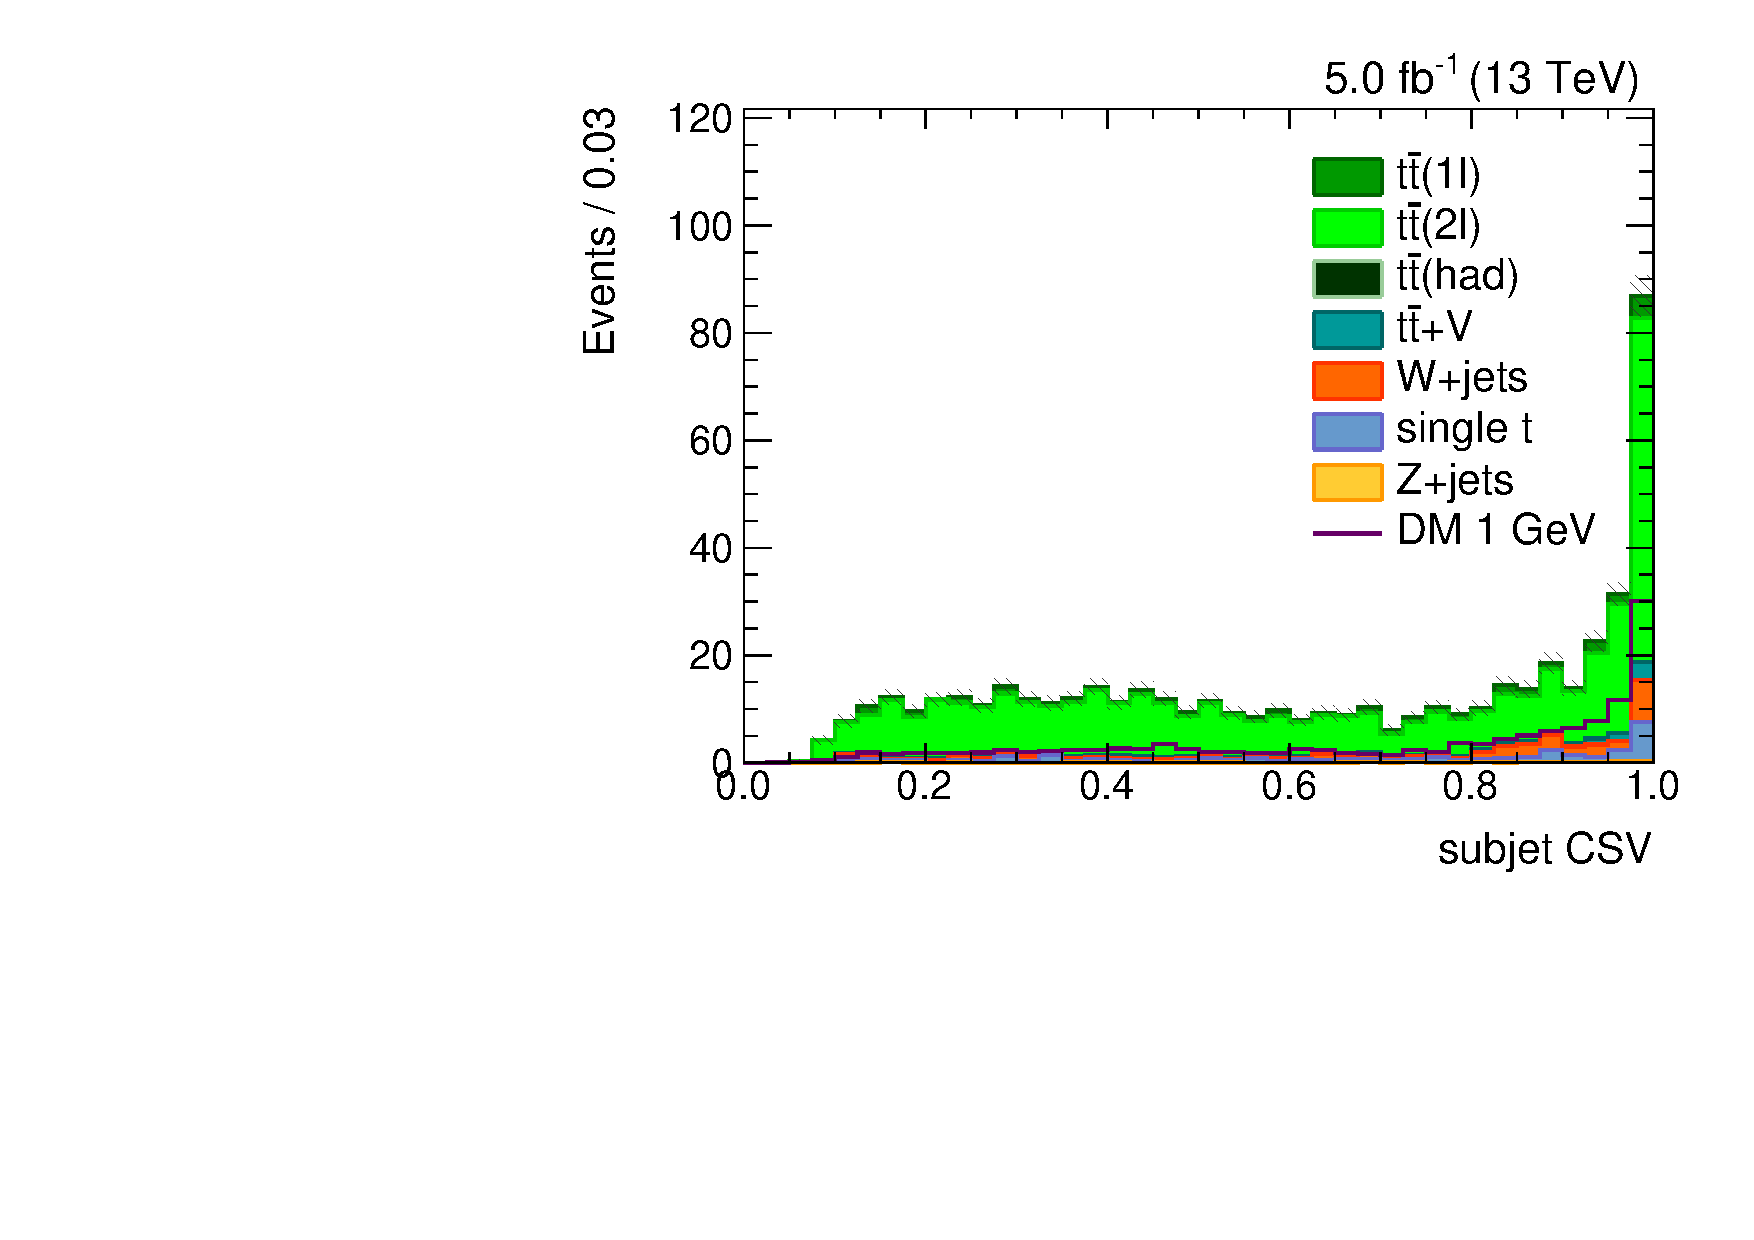
\includegraphics[width=0.48\textwidth]{figures/subjetbtag.pdf}
  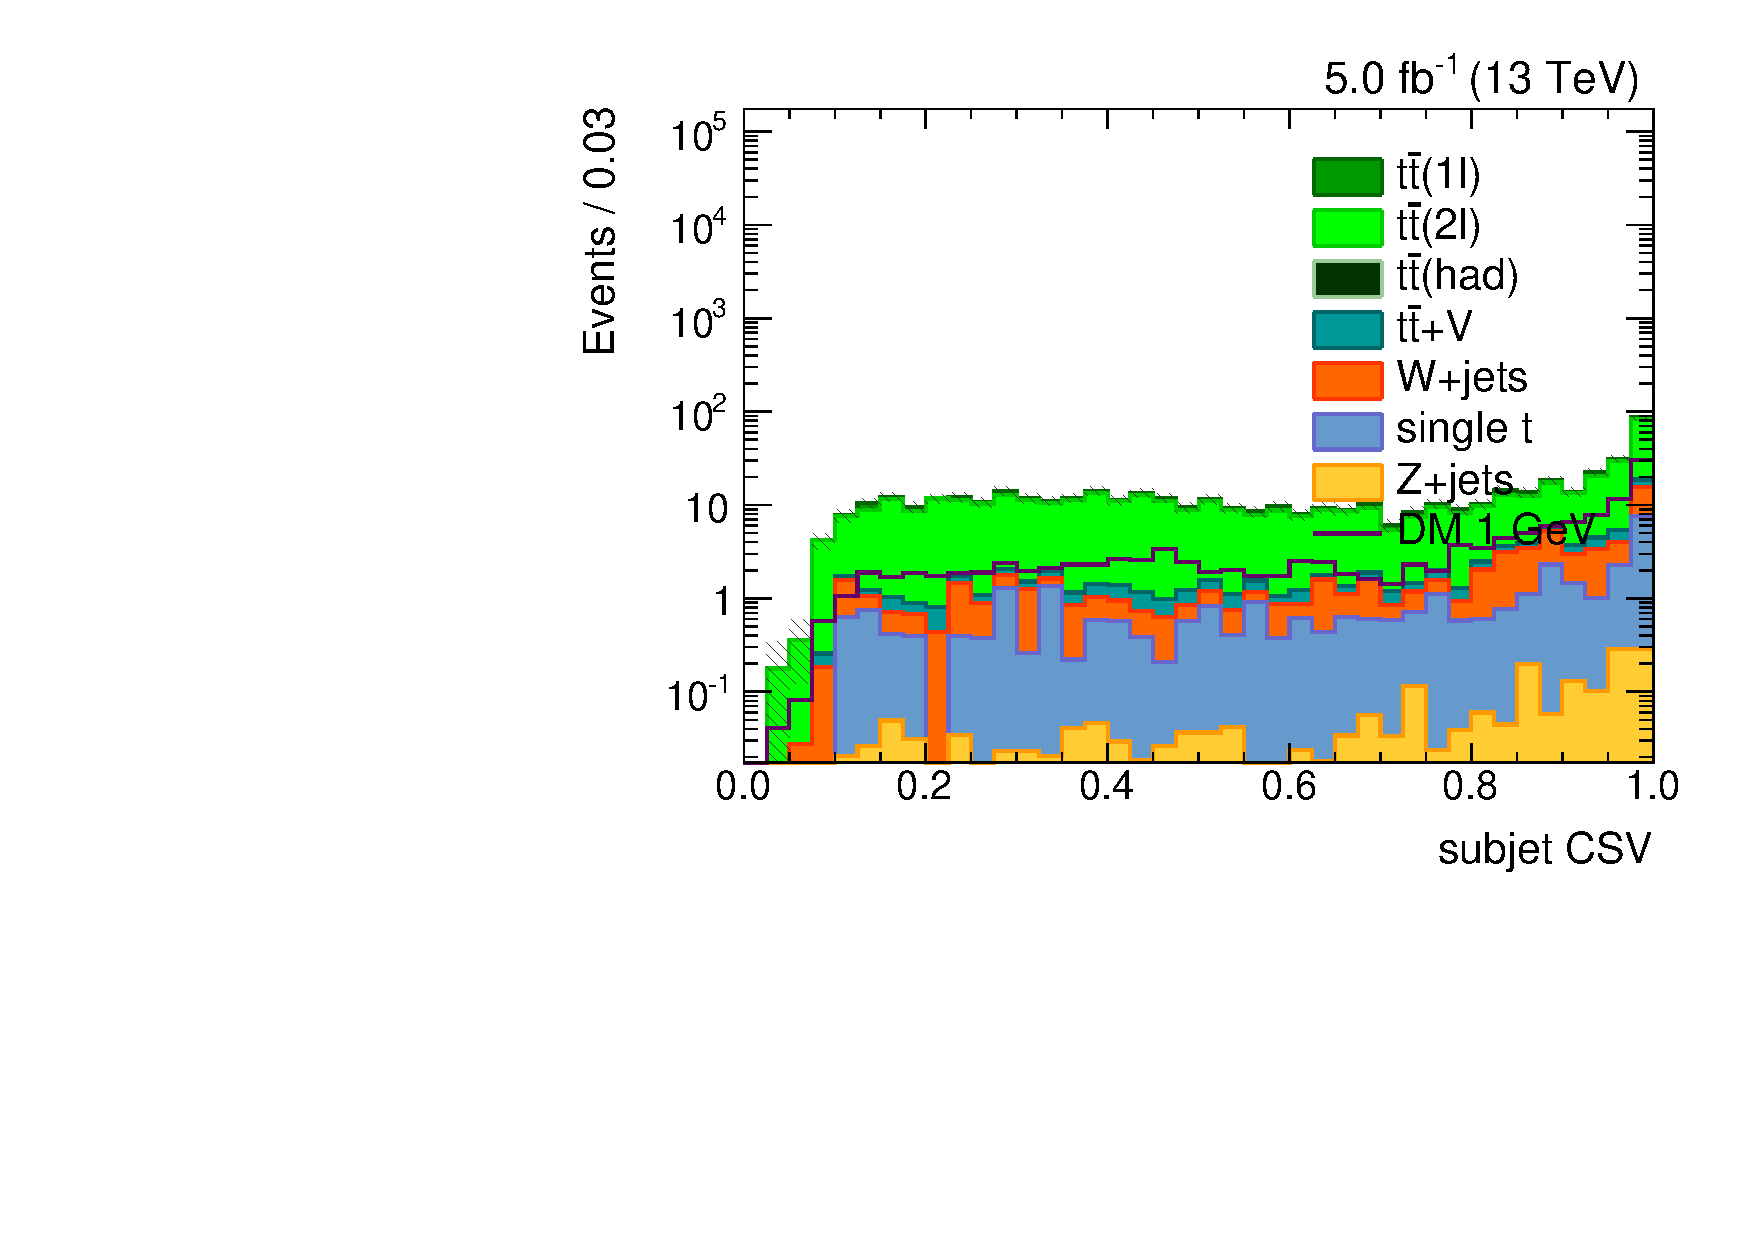
\includegraphics[width=0.48\textwidth]{figures/subjetbtaglog.pdf}
  \caption{Distribution of the largest CSVv2+IVF value among subjets in a wide jet. The wide jet must have $M_{\mbox{\scriptsize{soft drop}}}>75\:\GeV$.}
  \label{fig:subjet_btag}
\end{figure}

A boosted top is identified by the following requirements, 
\begin{itemize}
\item CA15CHS jet with $\pt>250\:\GeV$ and $|\eta|<2.4$,
\item $M_{\mbox{\scriptsize{soft drop}}} > 75\:\GeV$
\item $\tau_3/\tau_2 < 0.75$
\item maximum subjet $\Bot$-tag $> 0.4$
\end{itemize}

\clearpage
\subsection{Resolved Top Tagging}
\label{subsec:sel_toptag_resolved}

This analysis relies on the identification of resolved top decays. The resolved top decays are defined as consisting of three jets, each separately clustered by the anti-$k_{T}$ algorithm with size parameter R = 0.4. These AK4CHS jets employ charged hadron subtraction to reduce pileup contamination. Each jet is required to have a $\pt$ of at least $30\:\GeV$ and be located within the detector volume.

The resolved top tagging tool used in this analysis is a boosted decision tree (BDT) based multivariate discriminator (MVA), trained using the \textit{Toolkit for Multivariate Data Analysis with ROOT} (TMVA version 4.2.0) \cite{tmva}. The events selected for MVA training are from SM $\ttbar$ processes simulated in the Phys14 MC sample TTJets\_MSDecaysCKM\_central\_Tune4C\_13TeV-madgraph-tauola with a total cross-section of 831.76 pb. We use single lepton $\ttbar$ events and focus on the top where the W boson decays hadronically into two quarks which fragment and hadronize into jets. We permute all combinations of three jets from each event. Each jet from the tri-jet com bination is matched to a generator level parton which is within $\Delta R$ = 0.3 of the jet. 

The training of the MVA exploits the properties of the resolved top decay kinematics and jet identification properties. The jet properties used in the MVA training include a b-tagging discriminant value. This is determined via the most recent version of the \textit{Combined Secondary Vertex} algorithm (v2) together with the \textit{Inclusive Vertex Finder} algorithm (CSVv2+IVF). Although no explicit cut is applied on the b-tag discriminant for the selection of training events, we denote the jet with the highest CSVv2+IVF value as the b jet candidate. The remaining two jets are denoted as candidates for the jets emitted by the hadronic decay of the W boson. Other variables used in the training include the \textit{Quark-Gluon Likelihood} value of each jet, a value that corresponds to whether a jet originated from a quark or a gluon. The opening angles between the resolved top decay jets are also used. These include the separation in $R$- and $\phi$-space between each W decay jet candidate and the b jet candidate. 

We also employ a kinematic fit to the selected combination of three jets, and from this extract a fit probability \cite{kinfit}. We consider the invariant mass of the system comprised of the two candidate jets for the hadronic decay of the W boson. We also consider the three-jet system which includes the b jet candidate. The invariant masses of the two- and three-jet systems are constructed and the four-vectors of the jets are allowed to vary within their respective uncertainties in order to satisfy the top quark and W boson mass constraints imposed. A minimized $\chi^{2}$ function is extracted from the convergence of the kinematic fit and translated into a probability of fit. 

The input variables used in the training of the resolved top tagger include:
\begin{itemize}
\item jet CSVv2+IVF
\item jet quark-gluon likelihood (QGL)
\item $\Delta R$ ( hadronic W decay jet$_{\mbox{\scriptsize{1,2}}}$, b jet )
\item $\Delta \phi$ ( hadronic W decay jet$_{\mbox{\scriptsize{1,2}}}$, b jet )
\item fit probability 
\end{itemize}

and the jets selected for training satisfy the following requirements: 
\begin{itemize}
\item 3 AK4CHS jets with $\pt>30\:\GeV$ and $|\eta|<2.4$	
\item $100\:\GeV<M_{\mbox{\scriptsize{jjj}}}<300\: \GeV$
\end{itemize}

The MVA is trained with 100,000 signal events and 200,000 background events using the decision tree method which implements the \textit{GradientBoost} algorithm. A \textit{shrinkage} parameter, the learning rate for the GradientBoost algorithm, of 0.05 is specified. The small shrinkage necessitates the growth of more decision trees, but can significantly improve the accuracy of a prediction in difficult settings.

Input training variable correlations are shown in Fig.~\ref{fig:corr}. As expected, the kinematic angles $\Delta R$ and $\Delta\phi$ between the W decay candidate jets and the b jet candidate are correlated strongly in the signal, and less so in the background. 

\begin{figure}[htbp]
	\centering
	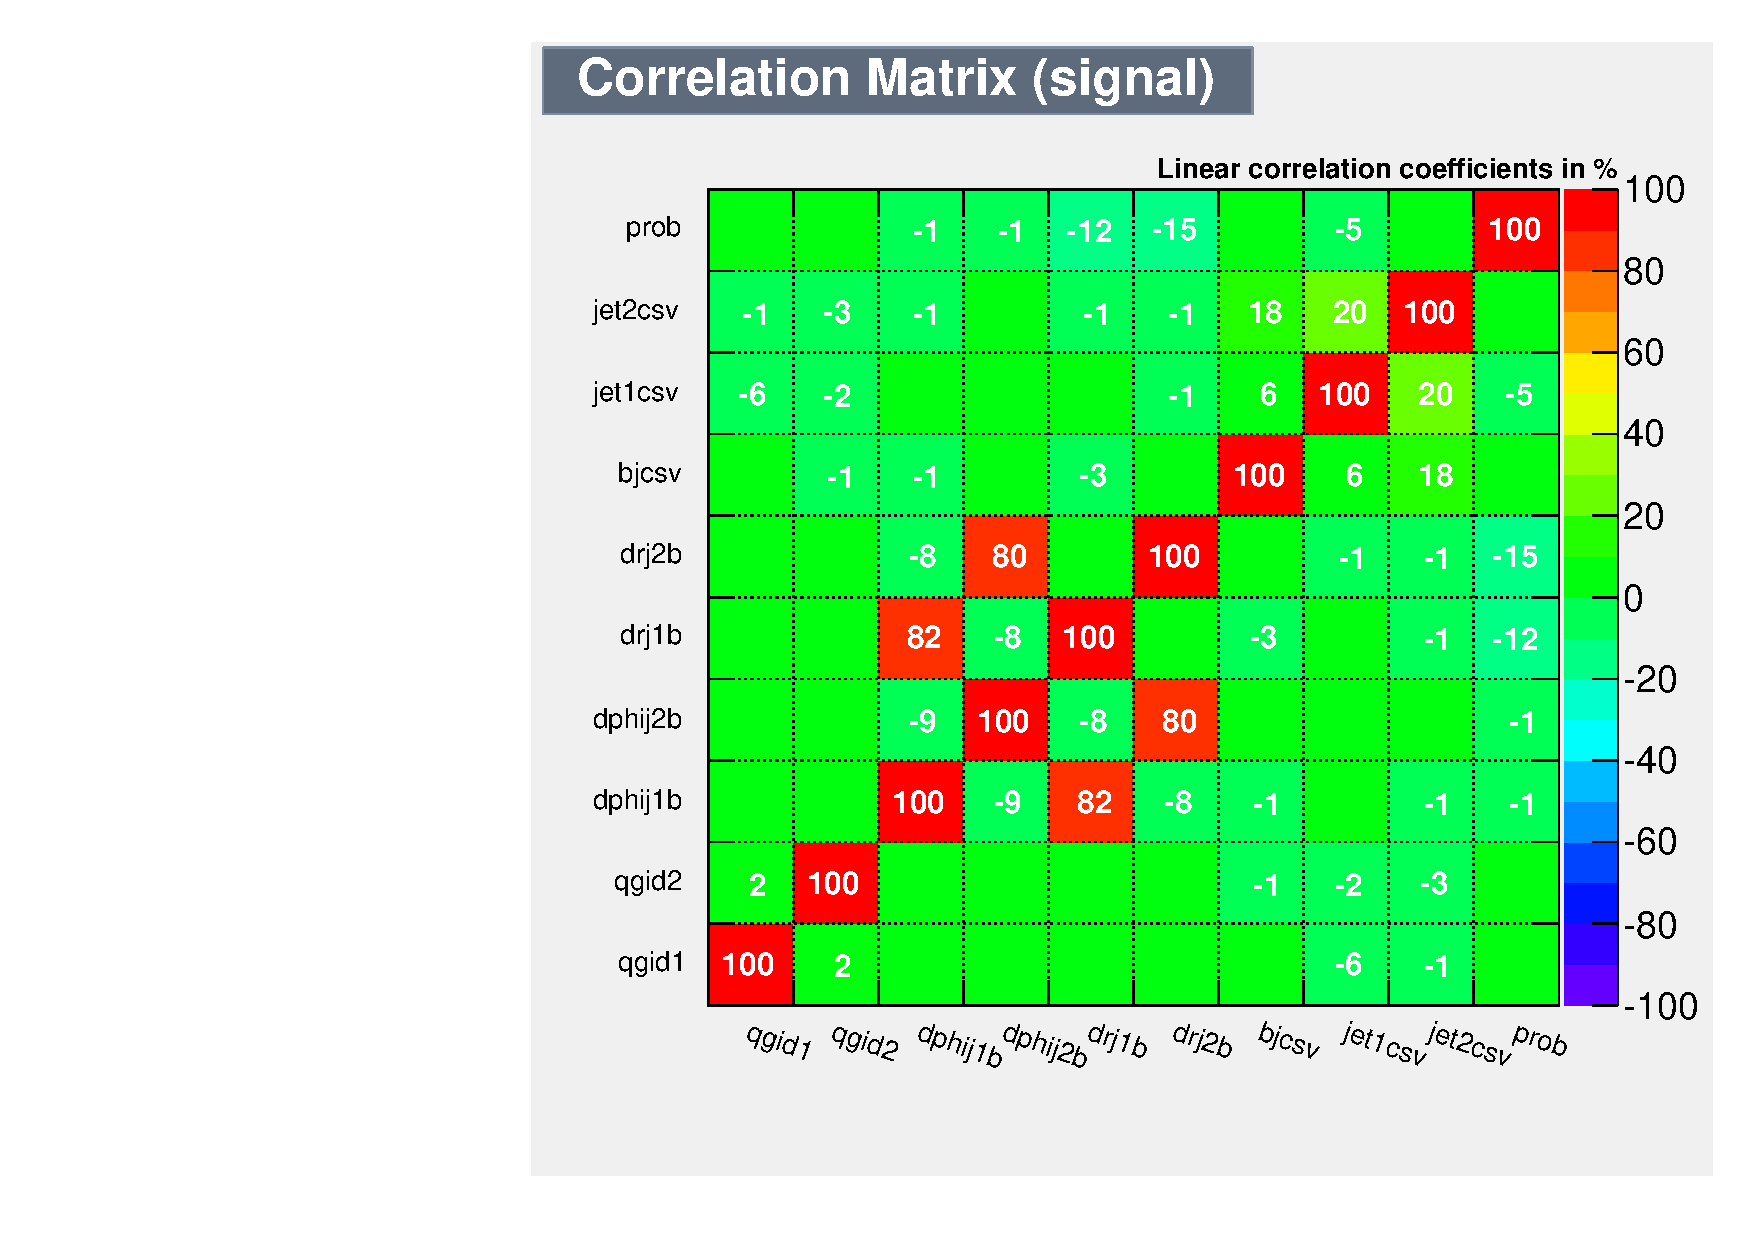
\includegraphics[width=0.48\textwidth]{figures/CorrelationMatrixS.pdf}
	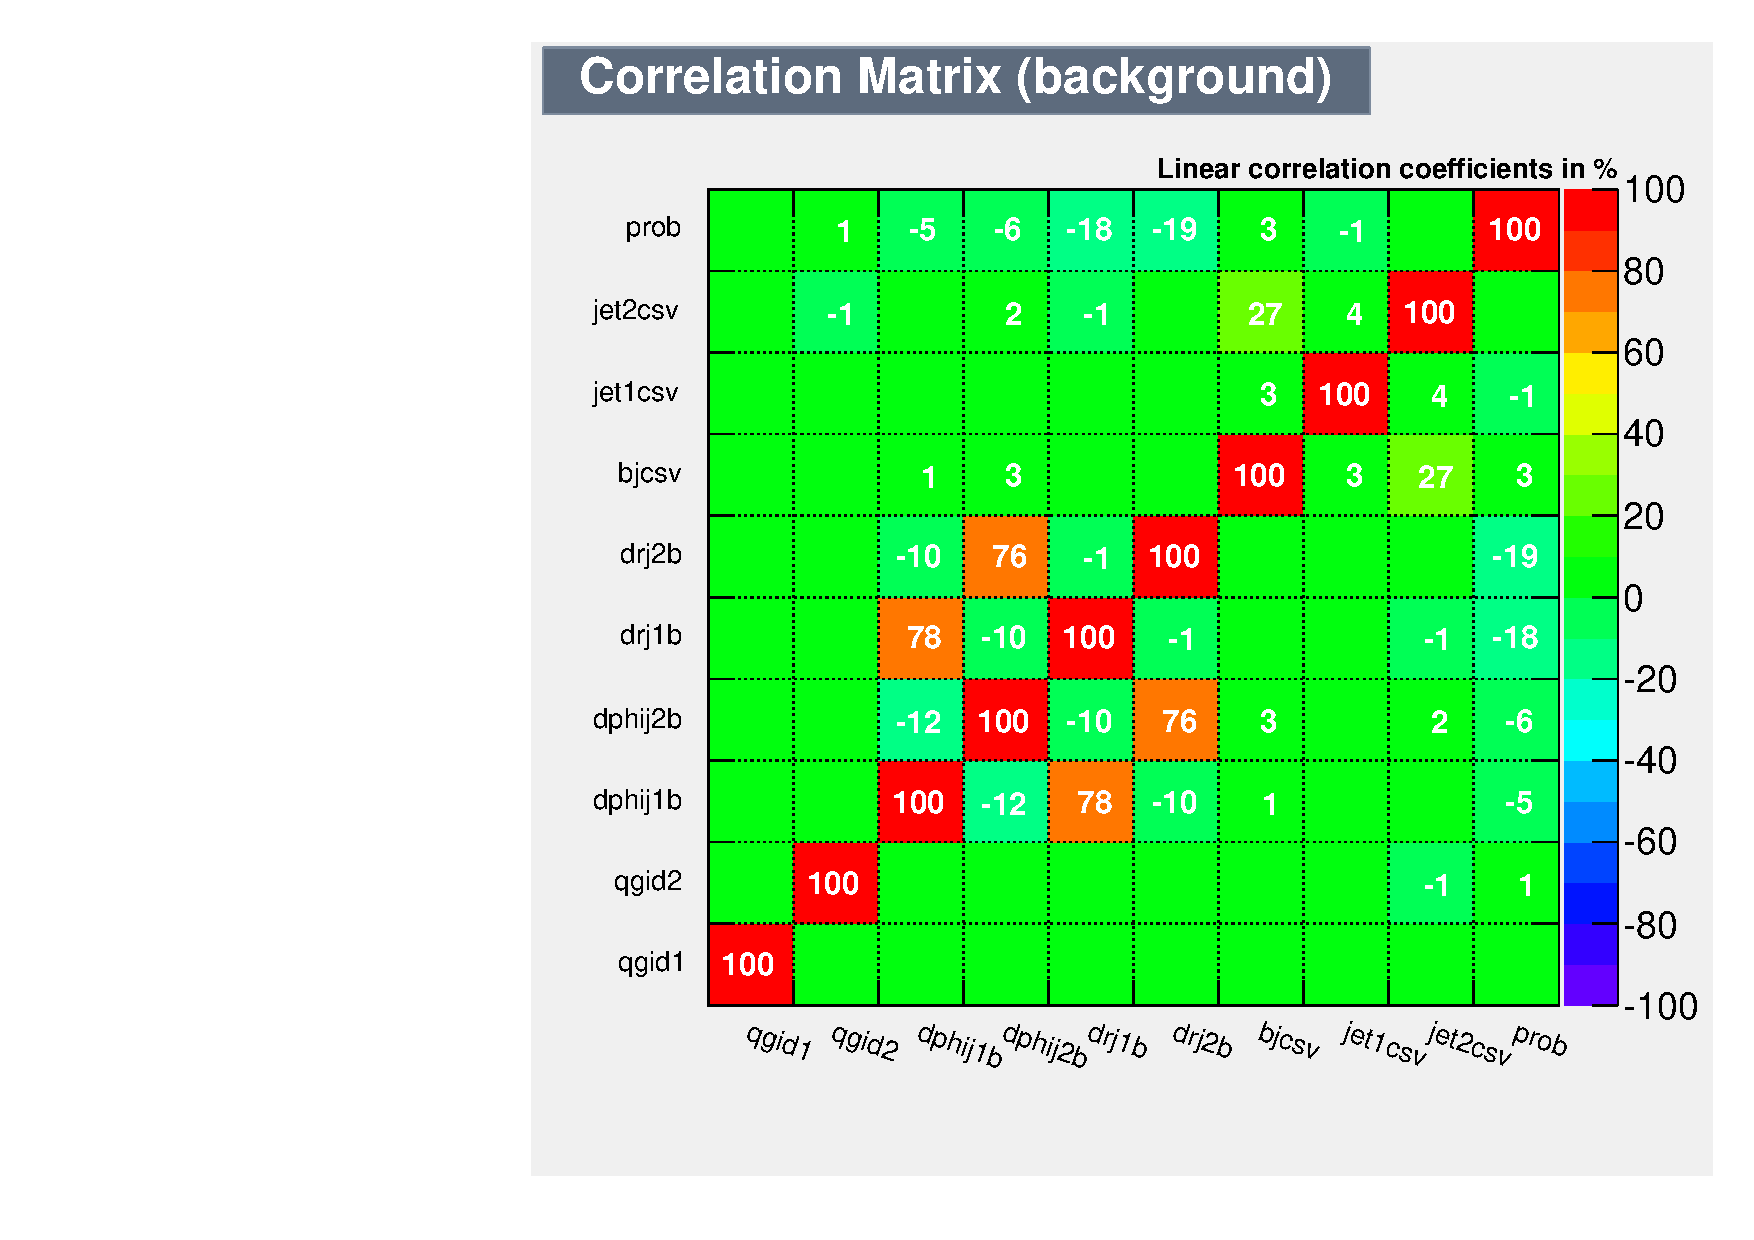
\includegraphics[width=0.48\textwidth]{figures/CorrelationMatrixB.pdf}
	\caption{Correlations between MVA input variables for signal and background}
	\label{fig:corr}
\end{figure}

The performance of the resolved top tagger is evaluated in single lepton $\ttbar$ events and $\Z\To\Nu\Nu$(+jets) events. Unique subsets of the same SM $\ttbar$ MC sample are used to train and test the MVA. A single event can contribute multiple background combinations, thus the tagger is evaluated using the background combination which has the highest output MVA score.

\begin{figure}[htbp]
	\centering
	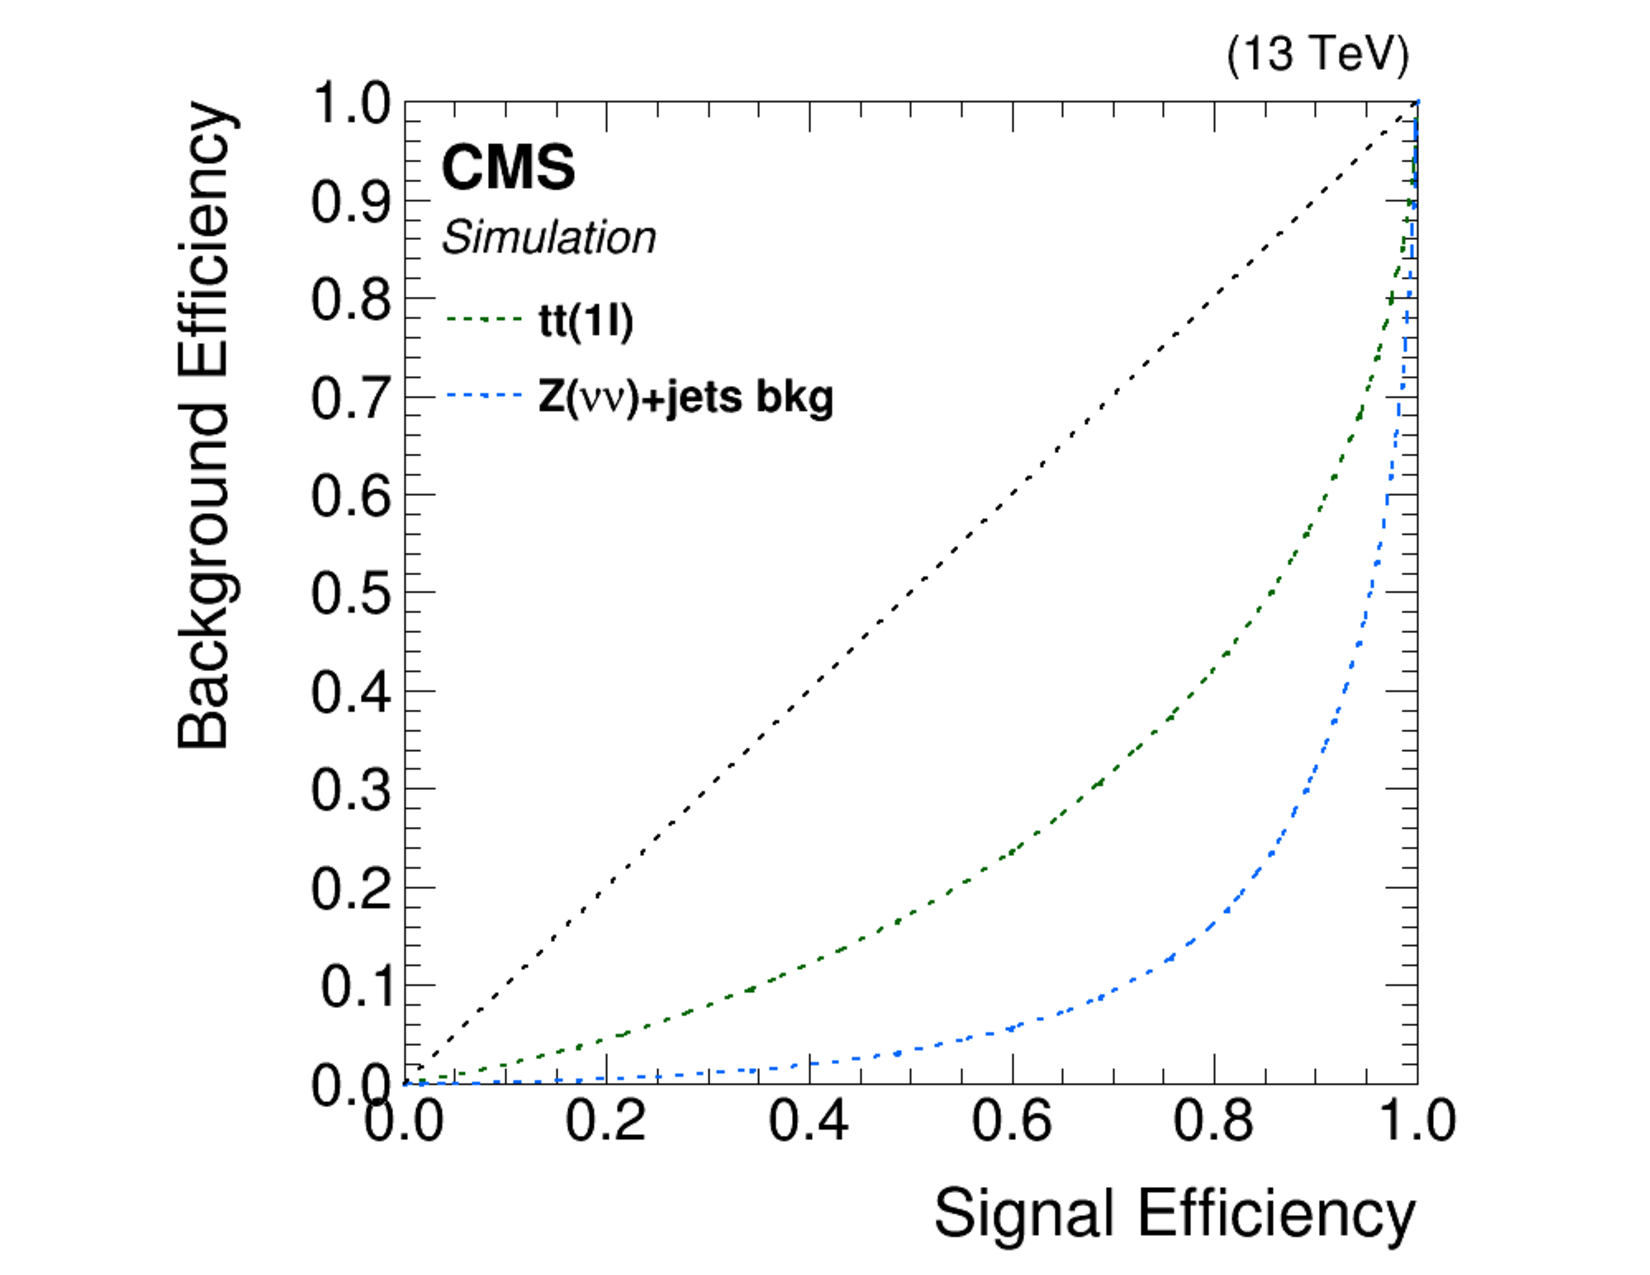
\includegraphics[width=0.48\textwidth]{figures/roctt1lzjets.pdf}
	\caption{Background  vs. signal efficiencies for $\ttbar(1\Lep)$ and $\Z\To\Nu\Nu$(+jets)}
	\label{fig:rocres}
\end{figure}

The efficiency behaviour of the resolved top tagger with respect to increasing top quark \pt\:\ was studied in MC. The efficiency in $\ttbar(1\Lep)$ events, the mistag rate of the $\ttbar(1\Lep)$ combinatoric background, and the mistag rate of $\Z\To\Nu\Nu$ events are shown as a function of the generator level top quark \pt\:\ in Fig.~\ref{fig:eff}. A working point corresponding to an approximate signal efficiency of 60$\%$ in $\ttbar(1\Lep)$ events was chosen as an illustrative benchmark. Limited statistics are available in the high top \pt\:\ regime.

\begin{figure}
	\centering
	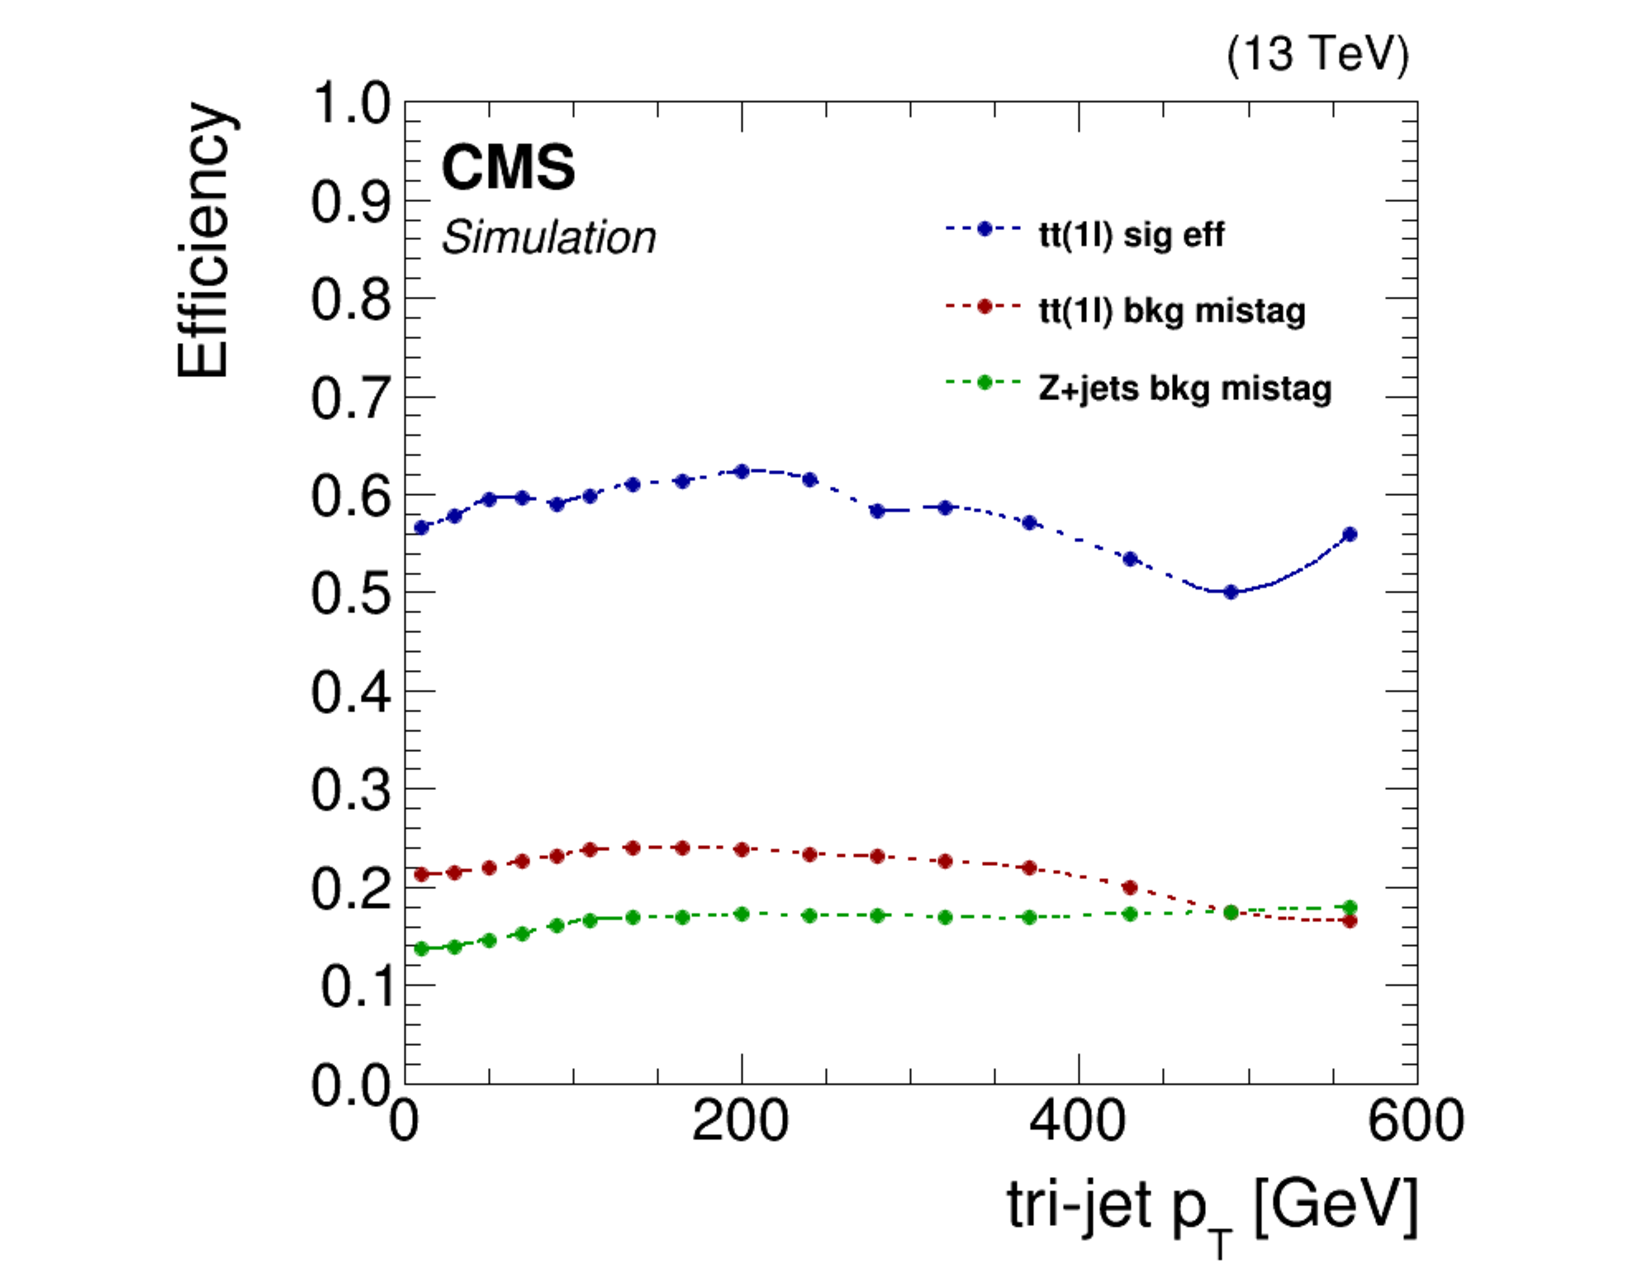
\includegraphics[width=0.48\textwidth]{figures/baseMVA+prob_bkg_effvspt.pdf}
	\caption{Resolved top tagger efficiency and mistag rates in $\ttbar(1\Lep)$ and $\Z\To\Nu\Nu$(+jets) Phys14 MC samples as a function of generator level top quark \pt\:\ and tri-jet \pt\:\ respectively}
	\label{fig:eff}
\end{figure}

The performance of the resolved top tagger was also characterized in 13\:\TeV\: data. Events for the study were selected using the HLT\_IsoMu27 trigger. The events satisfy the following offline selection criteria:

\begin{itemize}
\item exactly one muon passing ``Tight" selection with $\pt>30\:\GeV$ and $|\eta|<2.4$ 
\item $\met>100\: \GeV$
\item $M_T>40\: \GeV$
\item at least three AK4CHS jets with $\pt>30\:\GeV$ and $|\eta|<2.4$ 
\item at least two jets passing the``Medium" CSVv2+IVF WP 
\end{itemize}

The MVA output score distribution for data and MC is shown in Fig.~\ref{fig:score}. 

\begin{figure}[htbp]
	\centering
	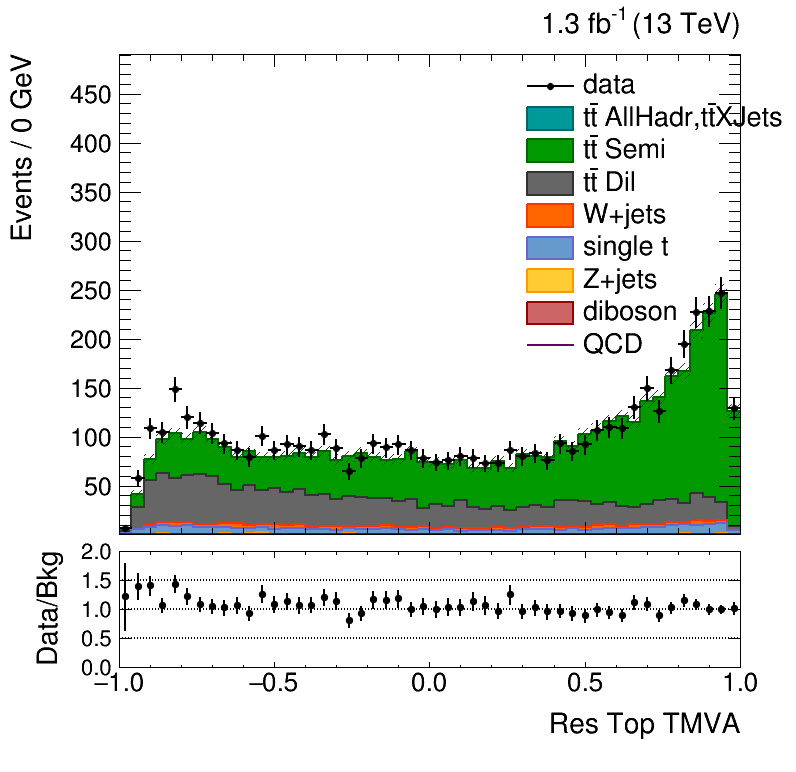
\includegraphics[width=0.48\textwidth]{figures/semilep_1tightmuo_resolved_3ormorejets_2ormorejetWPm_pfmetmore100_pfmtmore40_trigrequestonMC_qgsmearedwith8TeVrecipe_Oct302015/hResTopMVAlinear.png}
	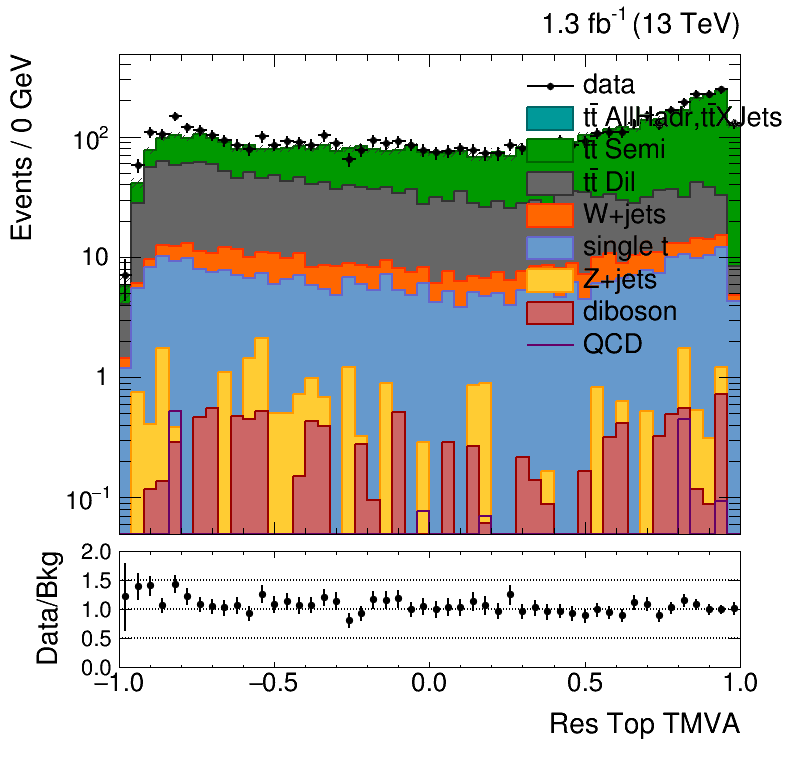
\includegraphics[width=0.48\textwidth]{figures/semilep_1tightmuo_resolved_3ormorejets_2ormorejetWPm_pfmetmore100_pfmtmore40_trigrequestonMC_qgsmearedwith8TeVrecipe_Oct302015/hResTopMVA.png}
	\caption{Resolved top tagger MVA output score distributions in data and MC in linear and log scale}
	\label{fig:score}
\end{figure}

Fair agreement is observed between data and MC, however better agreement is observed in 8\:\TeV\: studies, as described in Appendix ~\ref{app:8TeV}. The likely cause for the discrepancy at low MVA scores is due to the QGL which is currently under inverstigation (see Appendix ~\ref{app:TopTagger13TeVMore}).

In order to measure the efficiency and fake rates in data \footnote{Different efficiency/fake rate definitions used for training/characterization purposes (MC only) and scale factor measurements (data and MC comparison)}, the standard \textit{Tag and Probe} technique is employed \cite{TnP}. The semi-leptonic top candidate in the $\ttbar(1\Lep)$ event is taken to be the ``tag", while the ``probe" is the hadronically decaying top.
 The ``probe" is required to pass the aforementioned jet triplet selection. A passing ``probe" also passes the specified MVA score threshold, whereas a failing ``probe" will have an MVA output score lower than the specified threshold. The efficiency of the resolved top tagger is taken to be the number of passing ``probes" out of the total number of passing and failing ``probes".

In order to determine the yields in these categories, a simultaneous fit is performed in the orthogonal passing and failing ``probe" samples using the \textit{RooFit} framework. A $\ttbar(1\Lep)$ event can contribute either a jet triplet combination wherein each jet is matched to a generator level parton emitted from the hadronic top decay (signal) or a jet triplet combination with jets matched to underlying partons/combinatorial parton mismatch (background). Three  MC mass templates for the passing and failing ``probe" samples are constructed from:

\begin{itemize}
\item $\ttbar(1\Lep)$ signal events
\item $\ttbar(1\Lep)$ combinatorial background events
\item non-$\ttbar(1\Lep)$ background events (W/Z+jets, dibosons, single top, $\ttbar(2\Lep)$, hadronic \ttbar, \ttbar X(jets) )
\end{itemize}		 
	
The fit features six uncostrained nuisance parameters: 
\begin{itemize}
 \item signal rate in the inclusive (pass+fail) sample,
 \item combinatorial-background rate in the inclusive sample,  
 \item non-$\ttbar(1\Lep)$ background rate,
 \item signal efficiency ($\epsilon$), 
 \item combinatorial background fake rate ($FR1$) ,
 \item non-$\ttbar(1\Lep)$ background fake rate ($FR2$). 
 \end{itemize} 
 $\epsilon$, $FR1$, $FR2$ are defined respectively as the relative rates of passing ``probes" in signal, combinatorial-background, and non-$\ttbar(1\Lep)$ background.
 
 Results of the fit versus the chosen MVA score threshold is shown in Fig. \ref{fig:roofitresults13TeV}. Overall, we see good agreement, as in the 8 TeV data in appendix \ref{app:8TeV}.\\ 
  \textcolor{red}{Work on estimating the systematic uncertainties impacting the measurement.}
 
 \begin{figure}[htbp]
	\centering
	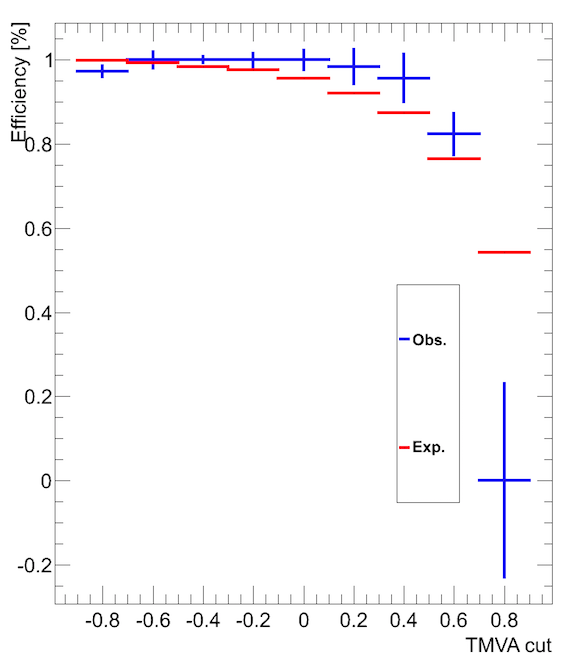
\includegraphics[width=0.48\textwidth]{figures/TOPRESOLVEDTAGGER_13TeV/c_eff.png}\\
	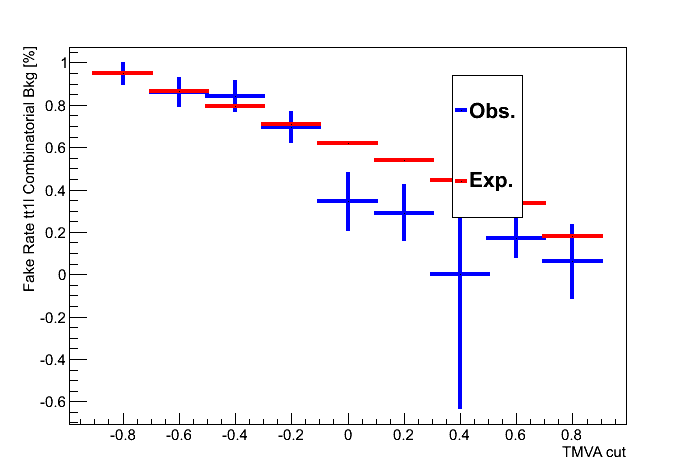
\includegraphics[width=0.48\textwidth]{figures/TOPRESOLVEDTAGGER_13TeV/c_fr1.png}
	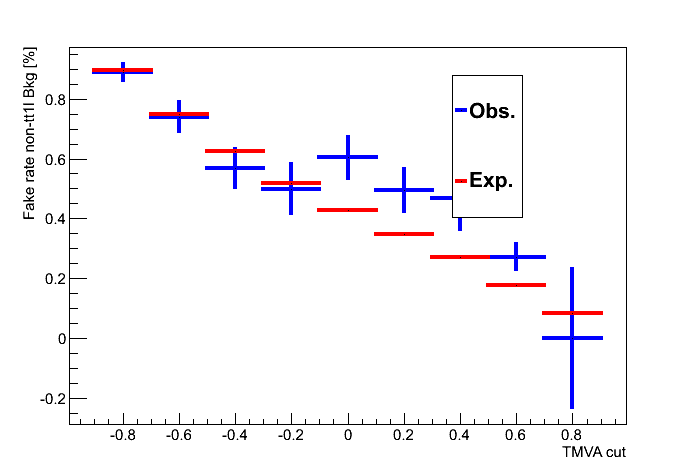
\includegraphics[width=0.48\textwidth]{figures/TOPRESOLVEDTAGGER_13TeV/c_fr2.png}
	\caption{Signal efficiency (top),  combinatorial background fake rate (bottom left), and non-$\ttbar(1\Lep)$ background fake rate (bottom right) in data (blue) and MC (red) as function of the MVA threshold. The procedure to estimate those quantities has been described in the text.}
	\label{fig:roofitresults13TeV}
\end{figure}



















\clearpage
\subsection{Top-tagged Selection: Hadronic channel}
\label{subsec:sel_toptag_hadronic}

In the hadronic channel, there can be up to two resolved \iffalse boosted \fi top tags in the event. \iffalse This naturally leads to definitions for three signal region categories: two top tags, one top tags, and zero top tags. \fi Events are required to pass the same trigger as in the inclusive selection (Sec.~\ref{subsec:sel_incl_hadronic}) and have $\met>250\:\GeV$,  $\min_{i=1,\ldots,6}\Delta\phi\left(j_i,\met\right)>0.6$, and two jet triplet combinations with resolved top MVA score $> 0.1$. In order to have two jet triplet combinations, we require at least six AK4CHS jets in order to obtain two hadronic top candidates.

%Then, the selections for the categories are as follows:
%\begin{enumerate}
%\item \emph{Boosted, Boosted}
  %\begin{itemize}
 % \item the two leading CA15CHS jets pass boosted top tagging requirements,
 % \item at least one AK4CHS jet is $\Bot$-tagged,
  %\item $\Delta\Phi_{i=1,\ldots,6}\left(j_i,\,\met\right)>0.6$.
  %\end{itemize}
%\item \emph{Boosted, Resolved}
%  \begin{itemize}
%  \item only one of the two leading CA15CHS jets pass boosted top tagging requirements,
  %\item at least $4$ AK4CHS jets in the event,
    %\begin{itemize}
    %\item at least $1$ of which have $|\eta|<2.4$ and $\Bot$-tagged,
   % \end{itemize}
 % \item $\Delta\Phi_{i=1,\ldots,6}\left(j_i,\,\met\right)>1$.
  %\end{itemize}
%\item \emph{Resolved, Resolved}
  %\begin{itemize}
    %\item Event passes the inclusive selection of Sec.~\ref{subsec:sel_incl_hadronic}.
  %\end{itemize}
%\end{enumerate}
\iffalse To ensure the categories are exclusive, the selections are applied in the order listed above and once the event satisfies the requirments of a particular category, it is no longer considered for subsequent categories.\fi The yields in the categories are shown Table~\ref{tab:toptag_hadronic_yields}.

\begin{table}[!ht]
\centering
\begin{tabular}{|c|r|r|r|}
\hline
  Process &\iffalse \multicolumn{1}{|c|}{Boosted, Boosted} & \multicolumn{1}{|c|}{Boosted, Resolved} &\fi \multicolumn{1}{|c|}{Resolved, Resolved} \\
\hline
  \Z\To\Lep\Lep           & \iffalse $ 0.02 \pm 0.01$ & $  0.35 \pm 0.09$ &\fi $  0.52 \pm 0.12$ \\
  \Z\To\Nu\Nu             &\iffalse  $ 4.82 \pm 0.18$ & $ 58.62 \pm 1.23$ &\fi $ 72.37 \pm 1.73$ \\
  Single \Top             &\iffalse  $ 1.00 \pm 0.41$ & $ 11.42 \pm 1.40$ &\fi $ 15.88 \pm 1.61$ \\
  \Wjets                  & \iffalse $ 3.55 \pm 0.34$ & $ 36.16 \pm 2.42$ &\fi $ 38.25 \pm 3.01$ \\
  QCD                     & \iffalse $ 0.00 \pm 0.00$ & $  0.00 \pm 0.00$ &\fi $  0.00 \pm 0.00$ \\
  $\ttbar+V$              & \iffalse $ 2.61 \pm 0.19$ & $  9.63 \pm 0.37$ &\fi $  5.37 \pm 0.28$ \\
  $\ttbar(\mbox{had})$ &\iffalse $ 0.00 \pm 0.00$ & $  0.00 \pm 0.00$ &\fi $  0.00 \pm 0.00$ \\
  $\ttbar(1\Lep)$         & \iffalse $15.85 \pm 1.61$ & $127.64 \pm 4.57$ &\fi $125.35 \pm 4.53$ \\
  $\ttbar(2\Lep)$         & \iffalse $ 1.14 \pm 1.88$ & $  6.86 \pm 1.06$ & \fi$ 18.47 \pm 1.74$ \\
\hline
  SM expected             & \iffalse $29.00 \pm 1.77$ & $250.69 \pm 5.61$ &\fi $276.21 \pm 6.18$ \\
\hline
  $M_\chi=1\:\GeV$        & \iffalse $61.86 \pm 1.60$ & $247.29 \pm 3.19$ & \fi$137.42 \pm 2.38$ \\
\hline
\end{tabular}
\caption{Expected yields for $5\:\ifb$ \iffalse in each category \fi after the top-tagged selection for the hadronic channel.\textcolor{red}{Plan to pursue boosted category for Moriond}}
\label{tab:toptag_hadronic_yields}
\end{table}

\clearpage
\subsection{Top-tagged Selection: Semileptonic channel}
\label{subsec:sel_toptag_semilept}

In the semileptonic channel, there are two signal region categories: one top tag and zero top tag. The zero top tag event selection is described in Sec.~\ref{subsec:sel_incl_semilept}. For the one top tag category, events are required to pass the same trigger and lepton requirements as in the inclusive selection (Sec.~\ref{subsec:sel_incl_semilept}), as well as have $M_{T}>160\:\GeV$ and $\met>160\:\GeV$. Thus the selection requirements, not including the previously mentioned trigger and lepton requirements are:

\begin{itemize}
\item $M_{T}>160\:\GeV$,
\item$M_{T2}^W > 200\:\GeV$,
\item$\min_{i=1,2}\Delta\phi\left(j_i,\met\right)>0.8$,
\item at least one of a minimum of 3 AK4CHS jets which passes ``loose" b-tag requirements,
\item resolved top MVA score $> 0.2$.
\end{itemize}

 %The selections for the categories are as follows:
%\begin{enumerate}
%\item \emph{Boosted}
%  \begin{itemize}
%  \item the leading CA15CHS jet passes boosted top tagging requirements,
 % \item at least one AK4CHS jet is $\Bot$-tagged,
 % \item $\Delta\Phi_{i=1,\ldots,2}\left(j_i,\,\met\right)>0.6$.
 % \end{itemize}
 %\begin{enumerate}
%\item \emph{Resolved}
%  \begin{itemize}
 %   \item Event passes the inclusive selection of Sec.~\ref{subsec:sel_incl_semilept}.
 % \end{itemize}
%\end{enumerate}
%\iffalse To ensure the categories are exclusive, an event is first considered for the Boosted category and then only considered for the Resolved category if it was not already selected.\fi 

The yields in the categories are shown Table~\ref{tab:toptag_semilept_yields}.

\begin{table}[!ht]
\centering
\begin{tabular}{|c|rr|r|rr|r|}
\hline
  & \multicolumn{3}{|c|}{Boosted} & \multicolumn{3}{|c|}{Resolved} \\
  Process & \multicolumn{1}{|c}{$e$} & \multicolumn{1}{c}{$\mu$} & \multicolumn{1}{|c|}{$e+\mu$} &
            \multicolumn{1}{|c}{$e$} & \multicolumn{1}{c}{$\mu$} & \multicolumn{1}{|c|}{$e+\mu$} \\
\hline
  \Z\To\Lep\Lep          &\iffalse $ 0.02 \pm 0.01$ \fi&\iffalse $ 0.11 \pm 0.06$ \fi& \iffalse $ 0.13 \pm 0.06$   \fi&   $  0.26 \pm 0.09$ & $  0.48 \pm 0.14$ & $  0.74 \pm 0.17$ \\
  Single \Top            &\iffalse $ 1.82 \pm 0.58$\fi & \iffalse$ 2.91 \pm 0.73$ \fi&\iffalse $ 4.73 \pm 0.93$   \fi&   $  6.84 \pm 1.11$ & $ 11.37 \pm 1.43$ & $ 18.22 \pm 1.81$ \\
  \Wjets                 &\iffalse $ 2.92 \pm 0.68$ \fi&\iffalse $ 4.71 \pm 1.22$ \fi& \iffalse$ 7.63 \pm 1.40$   \fi&   $  8.96 \pm 1.43$ & $ 13.93 \pm 2.26$ & $ 22.89 \pm 2.67$ \\
  $\ttbar+V$             & \iffalse$ 2.51 \pm 0.19$ \fi&\iffalse $ 2.90 \pm 0.20$ \fi&\iffalse $ 5.40 \pm 0.28$   \fi&   $  3.07 \pm 0.21$ & $  3.86 \pm 0.23$ & $  6.93 \pm 0.31$ \\
  $\ttbar(\mbox{had})$   &\iffalse $ 0.00 \pm 0.00$\fi & \iffalse$ 0.00 \pm 0.00$ \fi&\iffalse $ 0.00 \pm 0.00$   \fi&   $  0.00 \pm 0.00$ & $  0.00 \pm 0.00$ & $  0.00 \pm 0.00$ \\
  $\ttbar(1\Lep)$        & \iffalse$24.51 \pm 2.00$\fi &\iffalse $24.68 \pm 2.01$ \fi& \iffalse$49.19 \pm 2.84$   \fi&   $ 71.58 \pm 3.42$ & $ 89.72 \pm 3.83$ & $161.31 \pm 5.13$ \\
  $\ttbar(2\Lep)$        & \iffalse$ 2.45 \pm 0.63$\fi & \iffalse$ 2.78 \pm 0.67$ \fi& \iffalse$ 5.23 \pm 0.92$   \fi&   $  1.96 \pm 0.57$ & $  2.12 \pm 0.59$ & $  4.09 \pm 0.82$ \\
\hline
  SM expected            & \iffalse$34.23 \pm 2.29$\fi & \iffalse$38.08 \pm 2.56$ \fi& \iffalse$72.31 \pm 3.43$   \fi&   $ 92.68 \pm 3.92$ & $121.49 \pm 4.72$ & $214.17 \pm 6.13$ \\
\hline
  $M_\chi=1\:\GeV$       & \iffalse$28.88 \pm 1.09$\fi & \iffalse$35.91 \pm 1.22$\fi & \iffalse$64.78 \pm 1.63$   \fi&   $ 54.05 \pm 1.49$ & $ 67.33 \pm 1.66$ & $121.38 \pm 2.23$ \\
\hline
\end{tabular}
\caption{Expected yields for $5\:\ifb$ in each category after the top-tagged selection for the semileptonic channel.}
\label{tab:toptag_semilept_yields}
\end{table}

